%%% Hlavní soubor. Zde se definují základní parametry a odkazuje se na ostatní části. %%%

%% Verze pro jednostranný tisk:
% Okraje: levý 40mm, pravý 25mm, horní a dolní 25mm
% (ale pozor, LaTeX si sám přidává 1in)
\documentclass[12pt,a4paper]{report}
\setlength\textwidth{145mm}
\setlength\textheight{247mm}
\setlength\oddsidemargin{15mm}
\setlength\evensidemargin{15mm}
\setlength\topmargin{0mm}
\setlength\headsep{0mm}
\setlength\headheight{0mm}
% \openright zařídí, aby následující text začínal na pravé straně knihy
\let\openright=\clearpage

%% Pokud tiskneme oboustranně:
% \documentclass[12pt,a4paper,twoside,openright]{report}
% \setlength\textwidth{145mm}
% \setlength\textheight{247mm}
% \setlength\oddsidemargin{15mm}
% \setlength\evensidemargin{0mm}
% \setlength\topmargin{0mm}
% \setlength\headsep{0mm}
% \setlength\headheight{0mm}
% \let\openright=\cleardoublepage

%% Použité kódování znaků: obvykle latin2, cp1250 nebo utf8:
\usepackage[utf8]{inputenc}

%% Ostatní balíčky
\usepackage{graphicx}
\usepackage{amsthm}
\usepackage{fancyvrb}
\usepackage{fixltx2e}
\usepackage{tabularx}
\usepackage{rotating}
\usepackage[section]{placeins}

%% Balíček hyperref, kterým jdou vyrábět klikací odkazy v PDF,
%% ale hlavně ho používáme k uložení metadat do PDF (včetně obsahu).
%% POZOR, nezapomeňte vyplnit jméno práce a autora.
\usepackage[ps2pdf,unicode]{hyperref}   % Musí být za všemi ostatními balíčky
\hypersetup{pdftitle=Analysing and Visualizing  Statistical Linked Data}
\hypersetup{pdfauthor=Jiří Helmich}

%%% Drobné úpravy stylu

% Tato makra přesvědčují mírně ošklivým trikem LaTeX, aby hlavičky kapitol
% sázel příčetněji a nevynechával nad nimi spoustu místa. Směle ignorujte.
\makeatletter
\def\@makechapterhead#1{
  {\parindent \z@ \raggedright \normalfont
   \Huge\bfseries \thechapter. #1
   \par\nobreak
   \vskip 20\p@
}}
\def\@makeschapterhead#1{
  {\parindent \z@ \raggedright \normalfont
   \Huge\bfseries #1
   \par\nobreak
   \vskip 20\p@
}}
\makeatother

% Toto makro definuje kapitolu, která není očíslovaná, ale je uvedena v obsahu.
\def\chapwithtoc#1{
\chapter*{#1}
\addcontentsline{toc}{chapter}{#1}
}

\begin{document}

% Trochu volnější nastavení dělení slov, než je default.
\lefthyphenmin=2
\righthyphenmin=2

%%% Titulní strana práce

\pagestyle{empty}
\begin{center}

\large

Charles University in Prague

\medskip

Faculty of Mathematics and Physics

\vfill

{\bf\Large MASTER THESIS}

\vfill

\centerline{\mbox{
\includegraphics[width=60mm]{img/logo.eps}}}

\vfill
\vspace{5mm}

{\LARGE Bc. Jiří Helmich}

\vspace{15mm}

% Název práce přesně podle zadání
{\LARGE\bfseries Analysing and Visualizing \\Statistical Linked Data}

\vfill

% Název katedry nebo ústavu, kde byla práce oficiálně zadána
% (dle Organizační struktury MFF UK)
KSI

\vfill

\begin{tabular}{rl}

Supervisor of the master thesis: & Mgr. Martin Nečaský, Ph.D. \\
\noalign{\vspace{2mm}}
Study programme: & Informatics \\
\noalign{\vspace{2mm}}
Specialization: & ISS \\
\end{tabular}

\vfill

% Zde doplňte rok
Prague 2013

\end{center}

\newpage

Zadání

\newpage

%%% Následuje vevázaný list -- kopie podepsaného "Zadání diplomové práce".
%%% Toto zadání NENÍ součástí elektronické verze práce, nescanovat.

%%% Na tomto místě mohou být napsána případná poděkování (vedoucímu práce,
%%% konzultantovi, tomu, kdo zapůjčil software, literaturu apod.)

\openright

\noindent
I wish to thank my supervisor Mgr. Martin Nečaský Ph.D. for his time and his
very helpful and constructive advice concerning this thesis.

My thanks also belong to Bc. Martina Mandová who helped me
with the correction of the English text. I would also like to thank
my parents and my girlfriend for being supportive.

\newpage

%%% Strana s čestným prohlášením k diplomové práci

\vglue 0pt plus 1fill

\noindent
I declare that I carried out this master thesis independently, and only with the cited
sources, literature and other professional sources.

\medskip\noindent
I understand that my work relates to the rights and obligations under the Act No.
121/2000 Coll., the Copyright Act, as amended, in particular the fact that the Charles
University in Prague has the right to conclude a license agreement on the use of this
work as a school work pursuant to Section 60 paragraph 1 of the Copyright Act.

\vspace{10mm}

\hbox{\hbox to 0.5\hsize{%
In Prague date ............
\hss}\hbox to 0.5\hsize{%
signature of the author
\hss}}

\vspace{20mm}
\newpage

%%% Povinná informační strana diplomové práce

\vbox to 0.5\vsize{
\setlength\parindent{0mm}
\setlength\parskip{5mm}

Název práce: Analysing and Visualizing Statistical Linked Data

% přesně dle zadání

Autor:
Bc. Jiří Helmich

Katedra:  % Případně Ústav:
KSI
% dle Organizační struktury MFF UK

Vedoucí diplomové práce:
Mgr. Martin Nečaský, Ph.D., KSI
% dle Organizační struktury MFF UK, případně plný název pracoviště mimo MFF UK

Abstrakt:
Práce popisuje způsoby zpracování statistických dat v prostředí Linked Data, především s 
využitím metaformátu Data Cube Vocabulary. Její součástí je popis nástrojů, které 
souvisí s analýzou a vizualizací RDF dat nejen ze statistického 
prostředí. Nedílnou součástí je také popis nástroje Payola, na jehož vývoji se autor i nadále 
podílí. Výsledkem práce je zejména návrh a implementace systému, který 
umožňuje konverzi RDF dat dle slovníků Data Cube Vocabulary. Navržený 
systém byl implementován a integrován do aplikace Payola. Dále autor implementoval
několik dalších rozšíření tohoto systému. V rámci popisu implementace jsou zmíněna
také omezení vyplývající z integrace se systémem Payola.
V závěru práce autor popisuje několik experimentů, v jejichž rámci aplikoval 
implementovaný systém na vybrané datasety.

Klíčová slova:
% 3 až 5 klíčových slov
Linked Data, Data Cube, analýza, vizualizace, Payola

\vss}\nobreak\vbox to 0.49\vsize{
\setlength\parindent{0mm}
\setlength\parskip{5mm}

Title: Analysing and Visualizing Statistical Linked Data
% přesný překlad názvu práce v angličtině

Author:
Bc. Jiří Helmich

Department:
KSI
% dle Organizační struktury MFF UK v angličtině

Supervisor:
Mgr. Martin Nečaský, Ph.D., KSI
% dle Organizační struktury MFF UK, případně plný název pracoviště
% mimo MFF UK v angličtině
 
Abstract:
% abstrakt v rozsahu 80-200 slov v angličtině; nejedná se však o překlad
% zadání diplomové práce
The thesis describes several means of the process of statistical data in the ambience of Linked Data
and is in particular focused on the utilization of Data Cube Vocabulary metaformat.
Its content offers a description of tools related to analysis and visualization of RDF
data not only from the statistical view. An indivisible part of this work is the depiction of
the Payola tool on whose development is the author still working on. The outcome of this
thesis is mainly proposal and consequential implementation of the system that enables
a conversion of RDF data in compliance with the DCV vocabularies. The designed system
was implemented and integrated to the Payola application. Several other extensions of
the system were also implemented by the author. Within the scope of the implementation
process there are mentioned also limitations arising from the integration with Payola.
In the conclusion the writer describes a few experiments where some of the chosen
datasets were applied to the implemented system.

Keywords:
% 3 až 5 klíčových slov v angličtině
Linked Data, Data Cube, analysis, visualization, Payola

\vss}

\newpage

%%% Strana s automaticky generovaným obsahem diplomové práce. U matematických
%%% prací je přípustné, aby seznam tabulek a zkratek, existují-li, byl umístěn
%%% na začátku práce, místo na jejím konci.

\openright
\pagestyle{plain}
\setcounter{page}{1}
\tableofcontents

%%% Jednotlivé kapitoly práce jsou pro přehlednost uloženy v samostatných souborech
\chapter*{Introduction and motivation}
\addcontentsline{toc}{chapter}{Introduction and motivation}
\label{ch:preface}
Nowadays, there are many techniques of how to process data. Unfortunately, there are many
different data formats one can work with. It makes the~processing a~lot more difficult.
The task becomes even harder when one wants to connect two different datasets in order to
benefit from the~connection. The connection makes us able to get some additional information
about entities from each of the~standalone datasets. Therefore, a~lot of computation time is spent
on converting, formatting and transforming data into another form. But transforming datasets
into a~matching format is not enough. One needs to specify how the~data should be linked
together.

There are many ways of doing that. Starting with implementing the~logic into a~simple conversion
script (according to a~specific dataset) to introducing a~more complex metadata description
framework for purposes of generic data processing. Since one of the~most attractive
tasks in this area is to be able to connect any of the~datasets available on the~Internet,
we are interested in the~generic description frameworks. We would like to have 
a~tool, 
which makes us able to work with any data on the~Internet (formatted according to a~some
kind of rules). We would like to link them together, analyze them, visualize 
them.

One of the~most used description frameworks is the~Resource Description Framework~\cite{rdf}.
It is a~standard model for data interchange on the~Web. It tells us how to describe
resources on the~Internet in order to make other people, applications and tools
able to understand such a~description. That gives us the~potential to link any data on the~Internet.
Based on the~framework, a~new model named Linked Data~\cite{ld} was introduced. The model
has been brought up to make data interconnecting easier.

The result of interconnecting data while utilizing the~principles of the~Linked Data model
and Resource Description Framework is a~directed graph. Its vertices represent resources we
have information on. The edges stand for relations between such entities. From this point on,
it is up to us, how we look at the~data. We can either explore them in a~plain graph or apply
some more semantics and make domain specific visualizations while using ontologies
and other advanced techniques.

One of the~specific domains are statistical data, which are one of the~most interesting kind
of data. They are produced and processed by many stakeholders. In the~context of
\emph{Linked Open Data}, the~most interesting are, of course, governments and scientific groups.
But we would like to work with such data in the~usual
way --- make tables, charts or more interesting visualizations. While speaking about Open Data, a~specific
user group --- data journalists --- would like to work with Linked Data, but they are probably
missing some basic tools, which would make them able to interpret gathered results
in the~way readers would understand.

After applying the~rules of the~Linked Data model, the~statistical data (even tabular data)
get transformed into a~generic graph. The only, but very important advantage, is that we have some additional
metadata information available. Moreover, the~data are still linked with related entities from all over the Internet.
That brings
us to another model, the~Data Cube Vocabulary~\cite{dcv}. It is a~model, which tells us how to describe
multi-dimensional (statistical) data in respect to Linked Data and RDF 
principles.

\section{Goals of the~thesis}

The aim of this thesis is to describe these models, analyze the~possibilities of 
working
with multi--dimensional data in the~environment of Linked Data. We~will also propose a~system
which will make its user able to convert Linked Data into the~Data Cube Vocabulary model.
A prototype of such a~system will be implemented. An exemplary visualisation of the~statistical
data will be implemented and presented. Moreover, some missing Payola user interface features 
will be implemented.

\section{Structure of the~text}
In Chapter~\ref{ch:statistical-data}, we describe the aforementioned 
models and standards --- RDF, Linked Data, Data Cube and Data Cube Vocabulary. 
Some examples are presented. Chapter~\ref{chap:rw} contains description of 
existing tools and applications. We compare those to our application, Payola~\cite{payola}.
We also examine some related papers, especially the LDVM proposal~\cite{ldvm}. 
The Payola application is described in Chapter~\ref{ch:payola}. Later on (Chapter~\ref{ch:proposal}),
we propose a system
for analyzing and visualizing data compliant with the Data Cube Vocabulary model.
Implementation of a prototype is described in Chapter~\ref{ch:implementation}.
In Chapter~\ref{ch:experiments}, we present capabilities of the implemented system
and~experiment with some statistical datasets.
\chapter{Statistical data in the context of Linked Data}
\label{ch:statistical-data}
To understand the rest of the thesis, let us talk about the aforementioned models.
We will take the description step by step, starting with a dataset stored in a plaintext file.
After a while, we will get familiar with RDF, Linked Data and last, but not least, with the
Data Cube Vocabulary.

Since we are discussing statistical data, we will take a simple real--life example.
National statistical offices all over the world are well--known for periodic gathering of the
statistics about the population of the country they are operating in. Moreover, 
those statistics are being regularly published and gathered by international 
organizations, e.g. the UN~\cite{un} which can make a comparison and build 
another statistics upon the national data. Also, other organizations, like 
Google~\cite{pubdata} use those data to publish them and make 
some advanced statistics.

That is, in fact, why we would like to have the data in a pre--defined structure,
wrapped with metadata to perfectly understand what the data in a given 
dataset mean. Moreover, we would take advantage of such a dataset to speed up 
and automate its processing. It would be great to be able to introduce a tool, 
which will take the national statistics immediately after its publishing and 
deliver a new version of the international dataset without the need of any user 
input.

\section{From speech to structured data}

We will introduce the reader to the problem by examining an example based on the total number of
citizens living in the country. That is a very simple kind of information, but we will demonstrate
how this could be put into the context of the models mentioned in the introduction.

Let’s start with a dataset, which has only one entry:

\begin{verbatim}
The Czech Republic has 10 505 445 citizens.
\end{verbatim}

That’s a sentence a normal person would say but it holds a statistical information.
If we wanted to keep this information in a simple structured text file, we would e.g. name it
\texttt{number\_of\_citizens.txt} and it would have the following contents:

\begin{verbatim}
Czech Republic     10505445
\end{verbatim}

Normally, we keep this kind of statistics to make a comparison, 
for instance, to compare the total number of citizens of all the countries in the world.
We will, however, continue with just the two of them:

\begin{verbatim}
Czech Republic	    10505445
Slovakia	          5404555
\end{verbatim}

That gives us a dataset with two entries. Each entry is consisted of two parts. Let’s notice, that 
its semantics are kept in the reader's head. The document itself does not keep the information.
To process the data, it is necessary to know what the information in the file represents. You could change
the~contents of the file into the following form:

\begin{verbatim}
Czech Republic      10505445
Slovakia            5404555
Meat                like
Fruit               orange
\end{verbatim}

Such a dataset is technically correct (values are separated by tabulators), nevertheless 
semantically, it makes no sense. After reading the contents of the file, the reader 
is aware of the fact that in the given context the added lines do not fit in.
Let us return to the meaningful example.

If we keep the meaning of the values, we know that in the first column we have the name
of the country and in the second one, we have the total number of citizens. Those statements
could be called \emph{observations}, as it can be said that someone made an observation 
about there being over 10 million people living in the Czech Republic. We can also say that the
dataset has got two \emph{dimensions}. The first one is the place where the observation has taken
place, the second one is the value being measured.

That would make a nice Excel table, simple chart or a nice map of central Europe with
two labels. Those are the usual ways of processing such datasets.

Now, let us get back to the very first statement:

\begin{verbatim}
The Czech Republic has 10 505 445 citizens.
\end{verbatim}

When transferring the statement into a more technical form, we forgot to extract one
dimension. The sentence also carries information about time. This is quite an important
part of the information since the count of citizens of the specific country evolves with time.
People are dying as well as getting born. Since the sentence is presented while using the
present tense, we can conclude that the observation is valid for the current year (2013).

That means the dataset stored in a plaintext file should look similar to this:

\begin{verbatim}
Czech Republic       10505445     2013
Slovakia	            5404555      2013
\end{verbatim}

The last column evidently holds the year of the observation being made.
That gives us three dimensional dataset. We know the place, the total number of
citizens and the time of the measured value being acquired.

Now, we may come to a decision of publishing such a document to the Web. We can transform
it into a web page and publish it on a server.
\begin{figure}
\small\begin{verbatim}
<html>
    <head>
        <title>Number of citizens in a country</title>
    </head>
    <body>
        <table>
            <thead>
                <tr>
                    <th>Country name</th>
                    <th>Number of citizens</th>
                    <th>Year</th>
                </tr>
            </thead>
            <tbody>
                <tr>
                    <td>Czech Republic</td>
                    <td>10505445</td>
                    <td>2013</td>
                </tr>
                <tr>
                    <td>Slovakia</td>
                    <td>5404555</td>
                    <td>2013</td>
                </tr>
            </tbody>
        </table>
    </body>
</html>
\end{verbatim}\normalsize
\label{fig:rdf-html-01}
\caption{An example of an HTML file with tabular data}
\end{figure}

Example of such a web page source code can be seen in the 
figure~\ref{fig:rdf-html-01}. We published the data not only in a more structured form but also
provided an explanation of its meaning. Therefore, some additional data had to be added. In fact, we
should speak of it as of metadata, since the meaning is rather descriptive instead of semantical.

With a specifically programmed script or a tool (so-called \emph{scraper}) it is possible to
convert such a web page into another format or make an eye--catching visualization.
But one gets to learn the tool, the meaning of the data, its structures and the 
handling of each of the dimensions. Moreover, one is not able to gather more information,
because there is not any in the document itself and there is no way of
automatically linking the values in the document to other documents (unless, of course,
one is developed).

This is where the Resource Description Framework~\cite{rdf} and the Linked Data~\cite{ld}
model come in. Those
can help us to introduce some semantical meaning to link entities in the document to
other entities on the Internet. Let us provide more details about the RDF before getting
back to this example.

\section{Resource Description Framework}
As stated before, the Resource Description Framework is one of the most used models for
describing data with metadata. Its purpose is to give a common model for data interchange
on the Internet in order to make all its users able to exchange data with semantics.
It introduces a way of describing a schema of the interchanged data. It also 
offers features that help facing a situation when two datasets describe the same thing,
but have different schemas.

The standard model of the web works on the principle of URIs. Each page, which is, in fact,
an~entity or resource, has a URI, which stands for its unique identifier. Nothing on the web
should have the same identifier. What RDF adds to this model is that even relations
between those resources have their URIs. An example of such a relation could be:

\tiny\begin{verbatim}
http://dbpedia.org/resource/Kenya   http://www.w3.org/1999/02/22-rdf-syntax-ns#type http://dbpedia.org/ontology/Country  
\end{verbatim}\normalsize

This actually tells us that \texttt{Kenya is a country}. That statement could obviously be found on
the~Internet in a countless of different data sources; they are not usually presented
in a machine--readable form, though. In order to work with that sentence we need a 
parser, which is able to get the information based on a bunch of linguistical rules.
Moreso, the sentence might be more complicated, e.g. \texttt{Kenya, with Nairobi as its capital city,
is a very beautiful country}. Ignoring the fact that the sentence brings another useful
information, we should aim our focus on the fact that it is more of a complicated piece of language to parse. 

The RDF notation gives a semantic meaning to the relation. The RDF model is based on making certain
kinds of triples; such can be seen in the previous example. If we extend the set of triples with another,
what we get is \emph{a directed, labeled graph}, where an edge represents \emph{relation} between two resources.
Those resources are represented by graph nodes. Based on the actual content of the triples,
the~graph may consist of two or more standalone connected components as well as of
just a~single one. Such a graph may potentially contain information about entities from all over
the~Internet, which would be very useful.

The main point is, that all the information published in respect to the RDF model may be
automatically processed by a computer able to work with the semantics without
needing the user to specify it (as somebody has already done that while publishing the dataset).

\section{Linked Data}

A kind of implementation of the Resource Description Framework is the Linked Data model.
It utillizes several technologies and principles to actually interconnect the data on the Internet.
Both resources and relations are denoted with URIs. The HTTP protocol is used to make
the~resource public on the Internet. It may be found by dereferencing (accessing) the assigned
URI. Both machines and people are therefore capable of looking the resource up.

When the URI is dereferenced, more useful information could be provided while utillizing the RDF
and SPARQL standards. Since the model is called Linked Data, the most significant part
of the concept is about knowing how the data could be connected when being published on the Web.
It also brings some serialization formats, such as RDFa, RDF/XML, N3, Turtle and many others.
One of the most significant project involving Linked Data is the LOD2 project~\cite{lod2}.

To make the idea about datasets more clear, let us mention some well--known data sources
involving Linked Data:

\begin{itemize}
\item DBPedia --- dataset made by transforming Wikipedia into the RDF model.
\item FOAF --- dataset describing persons, their properties and relationships.
\item GeoNames --- geographical LD database.
\item CKAN --- community--run catalogue of useful sets of data on the Internet.
\end{itemize}

\subsubsection{Namespaces and prefixes}

There is one rather technical note we should mention before taking further steps. The RDF
also brings a way of expressing URI of a resource in a more compact form while utilizing
so--called prefixes and namespaces. Let us look at the example:

\scriptsize\begin{verbatim}
http://dbpedia.org/ontology/populationTotal
http://dbpedia.org/ontology/populationAsOf
\end{verbatim}\normalsize

Those are URIs which reference specific properties with a semantic meaning as designed
by the DBPedia~\cite{dbpedia}. At a closer look, one can see that there are some parts of the URI,
that are repeated in each of them. E.g. the scheme --- http. Although that is a rather technical
point of view. The most long common part of both URIs is \url{http://dbpedia.org/ontology/}
which makes a namespace. It makes a logical sense that all the resources in the virtual
folder \texttt{ontology} have something in common, therefore, they are grouped into the namespace.

Since one could remember easily the name of the specific resource in a namespace,
e.g. \texttt{populationTotal}, it would be great if they had no need to look up the full
URI of the namespace and express it with a short and easy--to--remember, but still 
unique, identifier. That’s what prefixes are designed for. For instance, the
\url{http://dbpedia.org/ontology/} was assigned the prefix \texttt{dbpedia-owl}. Since the scheme
is then \texttt{prefix:localname}, xone could write:

\scriptsize\begin{verbatim}
dbpedia-owl:populationTotal
dbpedia-owl:populationAsOf
\end{verbatim}\normalsize

which is equivalent to the previous example. It is then a lot easier to write RDF
documents for a human being, especially while using well--known prefixes. A kind of unofficial
registry could be found on~\cite{prefixcc}.

In order to get the processes in a country more transparent, governments also publish data
related to the country (statistics, public spendings data, …) to the Internet. Not many of
them are published in the form of the Linked Data, so there are many initiatives
interested in transforming the data into a machine-readable form.

It is definitely a great achievement to have such a dataset in a form of Linked Data, but
what we need for understanding its contents is a suitable visualization of the data.
Due to our knowledge of working with statistical multi--dimensional data we can apply our know--how
to the aforementioned data as they are statistical datasets as well.

\begin{figure}
	\centering
	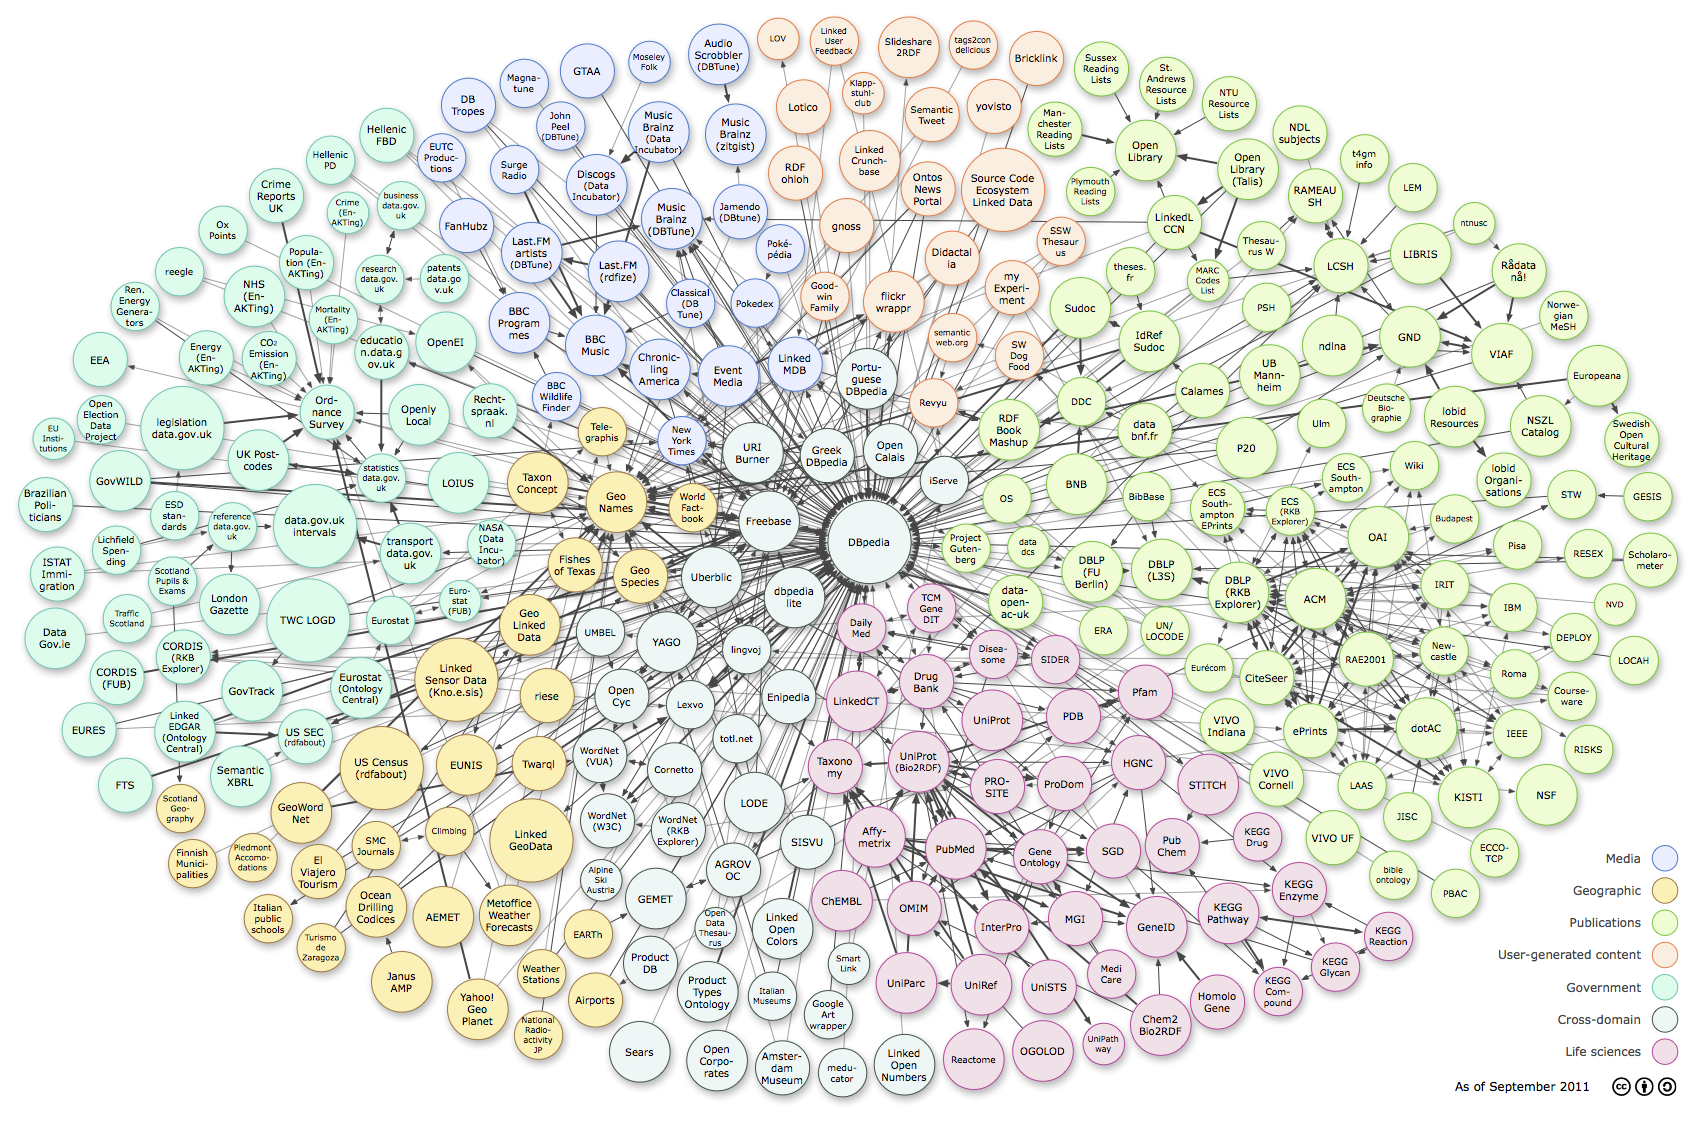
\includegraphics[width=150mm]{img/lod-cloud.png}
	\caption{LOD cloud diagram by Anja Jentzsch~\cite{lod-cloud} (situation as of 19. 9. 2011)}
	\label{fig:lod-cloud}
\end{figure}

Our aim is to have a description model, which annotates a dataset with a semantically--specific
notation. That would enable us to generalize the processes involving statistical Linked Data
and prepare some universal types of visualizations, which are commonly used in the non-LD world.

\subsubsection{Ontologies}

Let us also introduce the concept of an ontology, which is a product of the RDF evolution.
The Resource Description Framework is not very restrictive. One can build his own content
of a RDF document, e.g.:

\scriptsize\begin{verbatim}
http://example.com/Czech_republic	http://example.com/relation/hasCapital	http://example.com/Prague
\end{verbatim}\normalsize

or

\scriptsize\begin{verbatim}
http://pedia.rdf/Czech_republic	http://pedia.rdf/hasCapital	http://pedia.rdf/Prague
http://pedia.rdf/Czech_republic	http://pedia.rdf/language	http://pedia.rf/Czech
\end{verbatim}\normalsize

By comparing the first lines from each of the documents, it might be apparent they hold the same
information; that the capital city of the Czech Republic is Prague. At a closer look, a more observant
reader can notice, that each of them use different URIs to dereference the resources related to the
Czech Republic and Prague (in fact, they use different namespaces to make the reference).
They also use different URIs (and namespaces) to express the relation
between a country and its capital.

Moreso, the second document holds more information as it tells us, that people of the
Czech Republic speak Czech. Both documents are perfectly valid and could be 
published on the Web. That is why the concept of ontologies was introduced.
With an ontology, one may specify the requested outline of the document.

When formalized as defined in~\cite{ldvm2}:
\emph{An ontology $O$ is a triple $(C,P,M)$ where $C$ is a set of classes, $P$ is a set of
predicates and $M$ is a set of RDF statements (mappings of the classes and properties to
other ontologies). Both classes and predicates are specified using their unique URIs.}

Let’s start with countries. Without a restriction, one may also include, let us say, planets. With
an~ontology, it can be specified what kind of resources could be included.
It is needed to specify a URI describing the type \texttt{country}, for instance
a rule can be set that a resource needs to be of the type \mbox{\url{http://schema.org/Country}}.

After that, another rule is added, which will define that the country may have its capital
specified. Let’s say one decides to go with the relation described by dereferencing the URI of
\texttt{dbpprop:capital}. 

It is clear, that none of the examples conform, since neither of them utilizes the relation
\verb dbpprop:capital. This is a very simple example of how ontologies could be used. What we
did was, that we utilized the possibility to constraint properties of a resource.

A new language, OWL (Web Ontology Language)~\cite{owl}, was developed based on the RDF in order to
standardise the way of making restrictions. It gives us much stronger possibilities than just
restricting the properties, which is, on the other side, the most commonly used technique.

\subsubsection{Example with the usage of RDFa}

Now, let us get back to the example related to the number of citizens in a country. At first, we
will alter the HTML document to involve some semantics. To achieve that, we will utilize the
RDFa model, as can be seen in Figure~\ref{fig:example-rdfa}.

\begin{figure}
\scriptsize\begin{verbatim}
<html prefix="dbpedia-owl: http://dbpedia.org/ontology/">
    <head>
        <title>Number of citizens in a country</title>
    </head>
    <body>
        <table>
            <thead>
                <tr>
                    <th>Country name</th>
                    <th>Number of  citizens</th>
                    <th>Year</th>
                </tr>
            </thead>
            <tbody>
                <tr about=”http://dbpedia.org/page/Czech_Republic”>
                    <td property=”rdfs:label”>Czech republic</td>
                    <td property=”dbpedia-owl:populationTotal”>10505445</td>
                    <td property=”dbpedia-owl:populationAsOf”>2013</td>
                </tr>
                <tr>
                    <td property=”rdfs:label”>Slovakia</td>
                    <td property=”dbpedia-owl:populationTotal”>5404555</td>
                    <td property=”dbpedia-owl:populationAsOf”>2013</td>
                </tr>
            </tbody>
        </table>
    </body>
</html>
\end{verbatim}\normalsize
\caption{RDFa document example}
\label{fig:example-rdfa}
\end{figure}

Since the original data were taken from Wikipedia~\cite{wikipedia}, we decided to decorate the HTML document
while using semantic definitions defined by DBPedia, the Linked Data version of Wikipedia. 
The DBPedia needed to come up with a series of ontologies to present the structure of documents
extracted from Wikipedia. The ontology can be used not only to declare a publicly available definition of 
the document format, which is useful for those who query the DBPedia databse; it 
can also be used by the team of the DBPedia in order to unify internal rules of 
a document which is created by scraping a Wikipedia page into RDF.

As can be seen, we have utilized the RDF Schema and DBPedia Ontology to describe the document
and give it some semantic meaning. While this is a relatively simple process, it has dramatically
increased the possibilities of the document processing by expressing the resource dereference URI.
By dereferencing the URI, one can get more related information and link his data with the rest
of the Internet.

\subsubsection{RDF example}

When such a page is analyzed by a RDF--aware tool, it may be extracted into a more concise form:

\scriptsize\begin{verbatim}
http://dbpedia.org/page/Czech_Republic	dbpedia-owl:populationTotal		10505445 ;
                                       dbpedia-owl:populationAsOf		2013 .

http://dbpedia.org/page/Slovakia       dbpedia-owl:populationTotal		5404555 ;
                                       dbpedia-owl:populationAsOf		2013 .
\end{verbatim}\normalsize

The document may naturally contain much more information about the resources, but for the
purposes of our interest in the statistical values related to the population size we do not
need anything more. In fact, the DBPedia database contains many more data related to the entity,
e.g. the capital city, the name of the president, etc.

But all we need to start with statistical data in combination with the Linked Data concept is held
by those RDF triples. In fact, the main goal of this thesis is to implement a prototype of a 
system, which will be able to convert such triples (and more complicated statistical structures) into
slightly another, but still RDF--complaint, format.

\section{Data Cube}
\label{sec:datacube}
Before proceeding with the example, let us stop for a while and talk about Data Cube outside
the~RDF and Linked Data scope. Generally speaking, a data cube is a \emph{multi-dimensional}
 array of values describing some kind of data. In the
data--mining context, it is often referenced as an \emph{OLAP cube}, where OLAP stands for OnLine
Analytical Processing.

One may think about it as a generalization of a well--known concept --- spreadsheets.
A spreadsheet (known e.g. from the \emph{Excel}) is a two dimensional table, which can be
made dynamic while using formulas and other techniques available in the software. What
OLAP cube brings up is a higher count of dimensions. It holds a set of measures or, if you
want, observations. Those are organised in a special data structure (star schema, snowflake
schema, …) and points to so--called facts table consisted of the actual measured values.

While involving some facts from the database theory, we could say, that an OLAP cube is a form
of a projection of an \emph{RDBMS relation}. If we think about a standard two--dimensional table, we can
formalize the relation between key and value in the following way:

\begin{center}
$R = f: K \rightarrow V$
\end{center}

We have a single value (denoted \texttt{V}) that we get after dereferencing the key (denoted \texttt{K}).
If we add one dimension, e.g. let’s go back to the population count example, we would write:

\begin{center}
$R = f: (Y,C) \rightarrow V$
\end{center}

where \texttt{Y} stands for a year and \texttt{C} stands for a country. \texttt{V} is the total number of
citizens in the country \texttt{C} in the year \texttt{Y}.
But as we presented before, the OLAP cube represents a concept of
multi--dimensional statistical data. That’s why we should generalize the formula a lot more.
Let’s think about a cube which has n dimensions. That could be expressed with the following
formula:

\begin{center}
$R = f: (X_{1}, X_{2}, …, X_{n-1}) \rightarrow X_{n}$
\end{center}

But, of course, the $X_{n}$ could be also a set of facts.


\begin{figure}
	\centering
	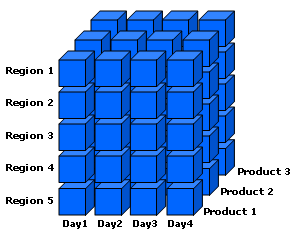
\includegraphics[width=100mm]{img/data-cube.png}
	\caption{An example of data cube by Microsoft~\cite{msdn-cube}}
	\label{fig:lod-cloud}
\end{figure}

The Data Cube Vocabulary is a concept based on the previously mentioned Data Cube and
OLAP cube theory. As we are interested in the ways of representing statistical data in the
Linked Data model, the reader would not be surprised, that the Data Cube 
Vocabulary~\cite{dcv}
concept is tightly connected to the Linked Data model.

Since the Data Cube Vocabulary is the starting point for reaching the goal of this thesis,
we will pay a special attention to its description. It combines the advantages of the RDF
model and Data Cube concept in order to make it easier to interlink resources involved
in the published statistics. As the Data Cube Vocabulary model is based on the model defined
by Statistical Data and Metadata eXchange standard~\cite{sdmx}, let us discuss the standard a bit more.

\section{Statistical Data and Metadata eXchange}
The SDMX Initiative~\cite{sdmx} was introduced by seven organizations in order to make
an~effective standard to interchange statistical data. All those organizations, e.g. OECD,
UN or Eurostat, have, without any doubt, access to a large amount of statistical data, even more,
they produce them. Some examples of such data could be found on~\cite{pubdata}.
In 2005, the Initiative has introduced a
version 1.0 of a technical specification, which was approved by the International
Organization for Standardization~\cite{iso} as \texttt{ISO:TS 17369}.
Later on, in May 2011, it was updated to version 2.1 (changes in web services guidelines,
revised data messages, partial code lists and new metadata management).
In January 2013 the specification has evolved into an International Standard,
\texttt{ISO/IS 17369}~\cite{isosdmx}.

The Initiative has also published a User Guide to cover major SDMX use cases~\cite{sdmxuserguide}.
It is focused on maintaining and handling statistical data and its metadata. It shows
how to manage reporting, storage, retrieval and extending. As a natural side--effect,
every organization, which follows the guide not only solves its problems with
handling the data, but is also able to interchange those with any other company
following the guide.

That corresponds with the idea of the RDF and Linked Data models. We have a large amount
of datasets we want to interchange or even interlink. Actually, it comes out of needs
of the founding organizations, which cooperate on the data they gather. Each of the companies creates
a~report, which is then processed or often even extended by one of the others. To make the chain
of the data processing more efficient, they agreed on the original technical specification.
They focused especially on the following issues detected in the statistical data exchange:

\begin{itemize}
\item Time consumption of the whole processing (data collection, transformations, 
exchange).
\item Different approaches introduced by different organizations.
\item Different approaches in how to utilize new technologies (like XML or web 
services).
\end{itemize}

While discussing the standard, several subprojects were introduced. One of them was to come
up with a standardized vocabulary for statistical metadata (metadata common vocabulary). It was
decided to use new technologies, such as web services or XML, but many of the subprojects
were based on existing concepts, which were utilizing existing technologies. In the case of
metadata common vocabulary, it was \emph{Eurostat’s Concept} and
\emph{Definitions Database (CODED)} and the \emph{OECD Glossary of Terms}.

The important result of the process is \emph{SDMX Content-Oriented Guidelines}.
They were separated
from the technical specification since they help to introduce some approaches to statisticians
for their work. The technical specification was focused on developing applications
conforming with the SDMX model. One could think that it is the technical specification
which enabled us to make the transition between common statistical data and Linked Data,
but it were the SDMX Content--Oriented Guidelines. On top of other products, it introduces the
following:

\begin{itemize}
\item Cross--Domain Concepts.
\item Cross--Domain Codelists.
\item Statistical Subject--Matter Domains.
\item Metadata Common Vocabulary.
\item SDMX--ML for the Content-Oriented Guidelines (Concepts, Code Lists, Category 
Scheme).
\end{itemize}

These are products that the Data Cube Vocabulary works with and builds upon. More important
features were added in the revision 2.0. The SDMX model was extended with reference metadata
concept which tells us how to format and structure metadata in respect to data quality
frameworks. Corresponding XML formats were introduced. Furthermore, a set of standard XML
interfaces was added to enable SDMX Registry manipulation. The registry was introduced to
enable data location catalogization and metadata cross--referencing over the Internet. Also,
structured metadata manipulation was introduced.

Since the SDMX Content--Oriented Guidelines are focused on SDMX use cases, we will present
one of them to the reader, since the same use case could be applied in the derived Data Cube
Vocabulary in the environment of Linked Data.

In fact, the primary use case designed by the Initiative is called “web data dissemination”
and is tightly related to the Linked Data world. It comes with a standardized process of retrieving
data from the web periodically and keeping them up--to--date. It resembles a bit a process
of scraping data into a Linked Data datastore, which was, perhaps, derived just from the web
data dissemination process.

The next SDMX fundamental connected to the Linked Data model is defining concepts. That is
very similar to the LD ontologies. A concept is a source of data semantics. It:

\begin{itemize}
\item Provides a detailed definition of the component, which describes the structure of the data or
metadata.
\item Can allow data and metadata for different structures to be comparable when concepts are reused.
\end{itemize}

The goal of SDMX is to reuse existing concepts introduced by any community related to the
given dataset, not to enforce its own proprietary format. It is enforced by a rule, which states
that a new concept can be introduced only if no existing concept suffices. The reason
is that those concepts are already used and implemented by a certain spectrum of
applications, therefore it will lead to a greater interoperability. Similar concepts are then
grouped into schemes which are versioned. When a concept changes, a new version of the
whole scheme needs to be introduced.

Also the list of three main components of SDMX concept goes well with the Linked Data model

\begin{itemize}
\item Its identification, which must be unique within the scheme.
\item Its name.
\item Its description.
\end{itemize}

One is also able to include all those properties into a RDF--compliant resource definition,
furthermore, the first one is also mandatory and represented by a URI.

\label{SDMX-code-lists}
Hand in hand with concepts goes defining code lists. It is a way of determining possible
values. In fact, those code lists are enumerations. They also have the three basic components
(identification, name and description) as concepts do. Code lists could be organized into
hierarchies to reflect a certain kind of relations between members of the list. The hierarchy
is meant to represent a children--parent relationship, but no additional properties are specified.
Let us mention \emph{Nomenclature des Unites Territoriales Statistiques (NUTS)} 
as an example of such a hierarchy.

The data definition reflects exactly what we need. It consists of a collection of 
components, which define what is being measured, together with additional metadata.

\section{Data Cube Vocabulary}
\label{datacube-vocabulary}

This model could be relatively easily decorated with syntactic sugar taken from the
RDF/LD world. This is exactly how the Data Cube Vocabulary was introduced based
on the model shown earlier. The most significant rule of the model is that each
dimension is needed to reference a concept to determine its semantic meaning.

But this is only a definition of a data structure, a set of rules of how a specific kind of information
should be published. Based on that, a dataset is published in a way to respect such a set
of rules. Therefore, every dataset represents a collection of data structures. Each data
structure is consisted of a set of components. One of them needs to be a measure,
a so--called \emph{primary measure}. The primary measure is marked with a special flag to be found
easily to enable more efficient processing.

Besides of measures, there are \emph{dimensions}. A data structure needs to have at least one.
Each dimension references its concept and has a unique identification. The combination of
all the dimensions (except the measure) defines a key, which makes it able to point
to the primary measure.

There are some kinds of specialized dimensions, which can be defined only once
for a data structure:

\begin{itemize}
\item Time (point in time, when the observation was made).
\item Measure (but could be a collection).
\end{itemize}

There are some preferred formats, which tell us, how to publish the time of capturing
the~observation --- a period, a duration or a timestamp. More details about that could be found
in the SDMX User Guide~\cite{sdmxuserguide}.

Moreover, a data structure can hold some metadata, e.g. the unit of the measurement
or a starting day of the week (in case of periodic time format).

As stated before, the SDMX 2.0 Information Model was used to build up the
RDF Data Cube Vocabulary, especially the Content--Oriented Guidelines (COGs). The Data Cube
vocabulary specification itself does not cover mechanics of transforming other formats
into the Data Cube Vocabulary, including the SDMX mostly used SDMX-ML. It presents the final
product, a model which builds upon the RDF and SDMX models.

In the section dedicated to the brief description of the RDF, we have discussed that resources
are identified by a unique identifier --- a URI. We have also mentioned that it is used to express
them in a compact form while utilizing prefixes and namespaces. Before going further with
the~description of the Data Cube Vocabulary, let us present a short list of significant prefixes
(presented in the Table ~\ref{tab:sdmxprefixes}),
since some of them could appear in the text.

\begin{table}[h]\footnotesize
  \caption{Prefixes used frequently with Data Cube vocabulary}
  \label{tab:sdmxprefixes}
\scriptsize\begin{tabular}{l l l}
Prefix & Namespace & Brief description \\
\hline
qb & \url{http://purl.org/linked-data/cube#} & Data Cube vocabulary \\
skos & \url{http://www.w3.org/2004/02/skos/core#} & Knowledge Organization Systems dictionary \\
scovo & \url{http://purl.org/NET/scovo#} & Statistical Core Vocabulary \\
void & \url{http://rdfs.org/ns/void#} & Vocabulary of Interlinked Datasets \\
foaf & \url{http://xmlns.com/foaf/0.1/} & People-related schemes \\
org & \url{http://www.w3.org/ns/org#} & Organizations dictionary \\
dcterms & \url{http://purl.org/dc/terms} & Dublin Core common properties dictionary \\
owl & \url{http://www.w3.org/2002/07/owl#} & Ontologies \\
rdf & \url{http://www.w3.org/1999/02/22-rdf-syntax-ns#} & RDF concepts \\
rdfs & \url{http://www.w3.org/2000/01/rdf-schema#} & RDF schema \\
eg & \url{http://example.org/ns#} & for examples only \\
pc & \url{http://purl.org/procurement/public-contracts#} & Public contracts \\
\end{tabular}\end{table}

The Data Cube vocabulary reuses the concept of a data structure as presented in the section
dedicated to the SDMX description. Therefore, a data cube is also consisted of a set of
dimensions, attributes and measures --- components, speaking generally. As in the cases of
OLAP cube and SDMX, dimensions are used to uniquely identify observed measures
(remember the formal mapping marking mentioned in the section about RDBMS representation
of OLAP cube). The outline of Data Cube Vocabulary can bee seen in the 
figure~\ref{fig:lod-cloud}.
 
\begin{figure}
	\centering
	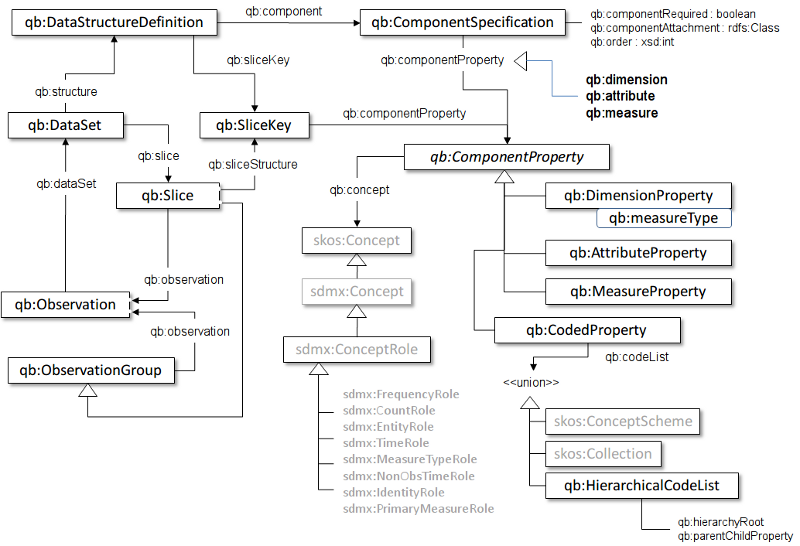
\includegraphics[width=150mm]{img/dcv-schema.png}
	\caption{Data Cube Vocabulary Outline~\cite{dcv}}
	\label{fig:lod-cloud}
\end{figure}

As a result, we are perfectly able to describe the measurement process - e.g., place, time and
other significant conditions, combined with the measured value itself. The whole information
is supplemented with additional attributes, which may make the measurement more accurate
- units, multipliers but also other, not so important, notes.

As we have discussed in the section dedicated to the SDMX model, each data set should be
published according to a specific data structure. Let us have a look on how the data structures are
modified by including Linked Data and let us try to create a data structure definition according
to our demography example.

A data structure definition is represented by \texttt{qb:DataStructureDefinition} resource. It defines
how the data set should be formed in order to comply with Data Cube Vocabulary. It defines
dimensions, attributes and measures, which may appear in the data set. Alongside with the
definition, optional and required attributes are defined, as well as their ordering. This kind
of information can be extracted easily from a well--formed document and need to not be explicitly
declared. But the explicit declaration enables you to:

\begin{itemize}
\item Verify the data set structure easily.
\item Determine what dimensions are available for a given data set.
\item Exchange structure definition.
\end{itemize}

\begin{sloppypar}
Since the data structure defines attributes, measures and dimensions, other resources need
to be involved. That is why \texttt{qb:ComponentProperty} class was introduced. It has a few derived
classes, \texttt{qb:DimensionProperty}, \texttt{qb:AttributeProperty}
and \texttt{qb:MeasureProperty}. Those carries
multiple pieces of information. Firstly, the concept, which is represented (e.g. time, place,
nation, currency, chemical substance, etc.) is followed by the type of the component
(dimension, attribute, measure). Last but not least, it carries the information about which
code list (see section~\ref{SDMX-code-lists}) is used to represent the value.
\end{sloppypar}

Since the goal of the SDMX model and Data Cube Vocabulary is to reuse community--proposed
taxonomies, \texttt{qb:concept} property was introduced to make it possible to link
\texttt{qb:ComponentProperty} with an existing concept. \emph{SKOS vocabulary} is used to
represent such concepts. SKOS does not define any specific concepts. It just defines
a~vocabulary for concept interlinking.

One could specify the range of the concept while defining a value of the \texttt{rdfs:range} property.
Also, the concepts may be used repeatedly in a data set in different roles.
For example, time could be used as a dimension (in the meaning that something was measured
in the year 2012) as well as a measured value (something took 203 seconds).

It is of a great help, if the value is a part of an enumeration defined in a code list. Due to
the~existence of the qb:codeList property, an automatic validation and range checking
can be performed. Moreover, tools can easily retrieve the complete list of possible values.
To enable range checking on non--coded values, rdfs:range can be used.

\begin{sloppypar}
Before getting back to our example, we need to point out a bridge between the SDMX
and Data Cube Vocabulary models. A community group has introduced some RDF 
encodings of SDMX COGs. These are \texttt{sdmx-concept}, \texttt{sdmx-code}, \texttt{sdmx-dimension},
\texttt{sdmx-attribute} and \texttt{sdmx-measure}. That is a simple way of interlinking the Data Cube
Vocabulary with the SDMX model.
\end{sloppypar}

Let us get back to the demography example. We will continue with the prepared RDF
document and transform it into a Data Cube Vocabulary model. Since we know that each
observation should conform to a specified data structure, we should at first define
such a structure. To define a structure, we need to define all components first.
We will use slightly modified examples presented in the Data Cube vocabulary
definition since it fits our use case:

\begin{enumerate}
\item Time definition [dimension]:

\begin{verbatim}
eg:refPeriod a rdf:Property, qb:DimensionProperty ;
    rdfs:label "reference period"@en ;
    rdfs:subPropertyOf sdmx-dimension:refPeriod ;
    rdfs:range interval:Interval ;
    qb:concept sdmx-concept:refPeriod .
\end{verbatim}

We define the \texttt{eg:refPeriod} and we state, that it is a \texttt{rdf:Property} and Data Cube dimension.
The rest of the statements are metadata, which are not really necessary, textual description
(label) and interlinking with existing concepts (relations to sdmx-dimension). To enable range
cheking, \texttt{rdfs:range} is defined.

\item Place definiton [dimension]:

\begin{verbatim}
eg:refArea a rdf:Property, qb:DimensionProperty ;
    rdfs:label "reference area"@en ;
    rdfs:subPropertyOf sdmx-dimension:refArea ;
    rdfs:range admingeo:UnitaryAuthority ;
    qb:concept sdmx-concept:refArea .
\end{verbatim}

\item Population count definiton [measure]:
\begin{verbatim}
eg:finalPopulation a rdf:Property, qb:MeasureProperty ;
      rdfs:label "the total number of citizens"@en ;
      rdfs:subPropertyOf sdmx-measure:obsValue ;
      rdfs:range xsd:decimal .
\end{verbatim}
\end{enumerate}

It is important to notice the link to the \texttt{sdmx-measure:obsValue}, which is the special flag
mentioned in the section dedicated to description of SDMX values. With the power of SPARQL
it is very easy to query a triple store to all the values, which are the observation values to get
all values in a given graph. In fact, it should be sufficient to query all instances of
\texttt{qb:MeasureProperty}, the relation to \texttt{sdmx-measure:obsValue} just makes the definition
more precise. An example of such a SPARQL query can be seen in the 
figure~\ref{fig:sparql-obsValue}.

\begin{figure}
\begin{verbatim}
  
  SELECT ?v WHERE {
    ?v a ?x .
    ?x rdfs:subPropertyOf sdmx-measure:obsValue .
  }

\end{verbatim}
\caption{A SPARQL query, which retrieves all observation values from a dataset}
\label{fig:sparql-obsValue}
\end{figure}

It is natural that while performing a measurement, you can retrieve multiple
values within a single observation. A good example of such an observation could be weather
information sampling. One can measure many physical values (e.g. temperature, air pressure,
humidity, …) in a specific timeframe on a specific place. One can store those values separately,
each in a standalone observation. But since the observation has been made in the same moment
and the dimensions are exactly the same, it is only natural to add those value components into
the~same observation. One will end up with a 5--dimensional observation where 2 components 
are dimension properties (place and time) and 3 components are measure properties
(temperature, pressure, humidity). Without grouping, one would make 3 related observations,
each with a single measure property (3 dimensions overall).

Regardless of whether you group those observations into a single one or not, one is able
to select the related observations from the data cube dataset relatively easily since they
are all determined by exactly the same dimension properties. That is called \emph{slicing}.
If you take a cube and select all the related observations you make a slice. The slice is exactly
the~same as the 5--dimensional observation mentioned before.

Based on the data structure, we can publish a specific dataset. The dataset could be formalized
as a collection of four data types:

\begin{itemize}
\item Observations --- values, measured numbers.
\item Organizational structure --- dimensions of the measured value (could be in the form of slices)
\item Internal metadata --- additional data description used to interpret observations (units, estimation,
etc.).
\item External metadata --- interlink to an author, dataset categorization, etc. (linked data 
principle).
\end{itemize}

An example of such a dataset can be seen in the 
figure~\ref{fig:example-dcv-dataset}.

\begin{figure}
\tiny\begin{verbatim}
@prefix rdf:     <http://www.w3.org/1999/02/22-rdf-syntax-ns#> .
@prefix rdfs:    <http://www.w3.org/2000/01/rdf-schema#> .
@prefix owl:     <http://www.w3.org/2002/07/owl#> .
@prefix skos:    <http://www.w3.org/2004/02/skos/core#> .
@prefix foaf:    <http://xmlns.com/foaf/0.1/> .
@prefix scovo:   <http://purl.org/NET/scovo#> .
@prefix void:    <http://rdfs.org/ns/void#> .
@prefix vcard:   <http://www.w3.org/2006/vcard/ns#> .
@prefix xsd:     <http://www.w3.org/2001/XMLSchema#> .
@prefix dcterms: <http://purl.org/dc/terms/>.

@prefix qb:              <http://purl.org/linked-data/cube#> .
@prefix sdmx:            <http://purl.org/linked-data/sdmx#> .
@prefix sdmx-concept:    <http://purl.org/linked-data/sdmx/2009/concept#> .
@prefix sdmx-dimension:  <http://purl.org/linked-data/sdmx/2009/dimension#> .
@prefix sdmx-attribute:  <http://purl.org/linked-data/sdmx/2009/attribute#> .
@prefix sdmx-measure:    <http://purl.org/linked-data/sdmx/2009/measure#> .
@prefix sdmx-metadata:   <http://purl.org/linked-data/sdmx/2009/metadata#> .
@prefix sdmx-code:       <http://purl.org/linked-data/sdmx/2009/code#> .
@prefix sdmx-subject:    <http://purl.org/linked-data/sdmx/2009/subject#> .

@prefix eugeo: <http://ec.europa.eu/eurostat/ramon/ontologies/geographic.rdf#> .

@prefix czso-teritorries:  <http://purl.org/cszo/teritorries#> .
@prefix czso-ds-dem-pop:   <http://linked.opendata.cz/resource/czso.cz/dataset/demography/final-population#> .
@prefix czso-ds-dem-bir:   <http://linked.opendata.cz/resource/czso.cz/dataset/demography/births#> .
@prefix czso-ds-dem-dea:   <http://linked.opendata.cz/resource/czso.cz/dataset/demography/deaths#> .
@prefix czso-ds-dem-imm:   <http://linked.opendata.cz/resource/czso.cz/dataset/demography/immigrants#> .
@prefix czso-ds-dem-emm:   <http://linked.opendata.cz/resource/czso.cz/dataset/demography/emmigrants#> .
@prefix czso-ds-def:       <http://linked.opendata.cz/resource/czso.cz/dataset-definitions#> .

czso-ds-dem-pop: a sdmx:DataSet ;
  dcterms:subject <http://eulersharp.sourceforge.net/2003/03swap/countries#cz>, <http://dbpedia.org/resource/Czech_Republic> ;
  dcterms:publisher <http://opendata.cz/me#> ;
  sdmx:maintainer <http://linked.opendata.cz/resource/business-entity/00025593> ;
  dcterms:date "2012-09-05"^^xsd:date ;
  qb:structure czso-ds-def:DemographyFinalPopulationDefinition .
  
czso-ds-dem-bir: a sdmx:DataSet ;
  dcterms:subject <http://eulersharp.sourceforge.net/2003/03swap/countries#cz>, <http://dbpedia.org/resource/Czech_Republic> ;
  dcterms:publisher <http://opendata.cz/me#> ;
  sdmx:maintainer <http://linked.opendata.cz/resource/business-entity/00025593> ;
  dcterms:date "2012-09-05"^^xsd:date ;
  qb:structure czso-ds-def:DemographyBirthsDefinition .
  
czso-ds-dem-dea: a sdmx:DataSet ;
  dcterms:subject <http://eulersharp.sourceforge.net/2003/03swap/countries#cz>, <http://dbpedia.org/resource/Czech_Republic> ;
  dcterms:publisher <http://opendata.cz/me#> ;
  sdmx:maintainer <http://linked.opendata.cz/resource/business-entity/00025593> ;
  dcterms:date "2012-09-05"^^xsd:date ;
  qb:structure czso-ds-def:DemographyDeathsDefinition .
  
czso-ds-dem-imm: a sdmx:DataSet ;
  dcterms:subject <http://eulersharp.sourceforge.net/2003/03swap/countries#cz>, <http://dbpedia.org/resource/Czech_Republic> ;
  dcterms:publisher <http://opendata.cz/me#> ;
  sdmx:maintainer <http://linked.opendata.cz/resource/business-entity/00025593> ;
  dcterms:date "2012-09-05"^^xsd:date ;
  qb:structure czso-ds-def:DemographyImmigrantsDefinition .
  
czso-ds-dem-emm: a sdmx:DataSet ;
  dcterms:subject <http://eulersharp.sourceforge.net/2003/03swap/countries#cz>, <http://dbpedia.org/resource/Czech_Republic> ;
  dcterms:publisher <http://opendata.cz/me#> ;
  sdmx:maintainer <http://linked.opendata.cz/resource/business-entity/00025593> ;
  dcterms:date "2012-09-05"^^xsd:date ;
  qb:structure czso-ds-def:DemographyEmmigrantsDefinition .
  
<http://linked.opendata.cz/resource/czso.cz/dataset/demography/final-population/554782-2011> a qb:Observation ;
    qb:dataSet <http://linked.opendata.cz/resource/czso.cz/dataset/demography/final-population#> ;
    czso-ds-def:refArea <http://linked.opendata.cz/resource/region/554782> ;
    czso-ds-def:refPeriod "2011"^^xsd:gYear ;
    czso-ds-def:finalPopulation "1241664"^^xsd:nonNegativeInteger .

<http://linked.opendata.cz/resource/czso.cz/dataset/demography/births/554782-2011> a qb:Observation ;
    qb:dataSet <http://linked.opendata.cz/resource/czso.cz/dataset/demography/births#> ;
    czso-ds-def:refArea <http://linked.opendata.cz/resource/region/554782> ;
    czso-ds-def:refPeriod "2011"^^xsd:gYear ;
    czso-ds-def:births "13968"^^xsd:nonNegativeInteger .
\end{verbatim}\normalsize
\caption{An example of a DCV dataset}
\label{fig:example-dcv-dataset}
\end{figure}

In this chapter, we have introduced a long process of transforming a simple statement into
a~form, which is compliant with the Data Cube Vocabulary standard. The original statement
was processed while applying a set of a simple transformation steps, at least from the point of view
of a human brain. The goal of this thesis is to make one of these steps as automatic as possible 
in order to come up with a prototype of a system, which is able to transform an arbitrary set of RDF data
into a Data Cube Vocabulary form, if possible. Also, a user input (a set of transformation rules) is
needed to get such a task done. 

Since Payola was designed to provide a platform for analyzing and visualizing 
Linked Data and its main goal is to lower the knowledge barrier, which one needs to 
overcome in order to analyze Linked Data, we also want all newly--introduced 
components to fit into the concept of the whole platform --- to be reusable. We 
will also demonstrate the benefits of such transformations while implementing 
a~visualization, which will take advantage of the Data Cube Vocabulary.
\chapter{Related Work}
\label{chap:rw}

In this chapter, we~would like to~get the~reader familiar with the~variety of~tools, which one can
use to~analyze and~visualize Linked Data. We~will naturally compare these tools with
Payola, since in~the~past we~participated on~the~proposal and~development of~this system.
Since the~goal of~this thesis is~to~propose and~implement a~system based on~the~Data Cube Vocabulary
standard we~will, at~first, focus on~tools with the~data cube support. 

We will provide a~well--arranged table in~order to~present a~quick overview of~what related tools are available at~the~time of~writing this thesis and~what are those 
tools capable of. Before we~come up~with the~table let us~mention, which~features are examined and~why.

The main goal of~this thesis is~to~deliver a~prototype of~a~system, which will map 
arbitrary RDF data to~a~form compliant with the~Data cube Vocabulary. Based on~this fact, one of~the~criteria is~an~ability to~\emph{convert arbitrary data 
into a~form of~cubes}. Another difference lies in~a~format of~\emph{input data} of~the
mapping process. There are tools working with relational (R), Linked Data (LD) or
arbitrary format (A).

The main benefit of~implementing such a~feature into~Payola is~that it~becomes a~part of~an~ecosystem. First of~all, we~have the~user make an~analysis over an~arbitrary
dataset (or, while using more than one data source even more than one dataset)
and then map it~into~the~Data Cube Vocabulary standard. That also means that one is~able
to analyze the~data, interconnect them, filter them and~enrich entities with more properties
while utilizing the~principles of~Linked Data before the~mapping is~made. Moreover, the~statistical
dataset could be~the~result of~an~analysis. A~new statistical dataset may originate from performing
such an~analysis. On~the~other hand, many of~the~existing 
tools provide a~way of~converting a~rather static dataset. Let us~imagine a~situation when a~user has a~database of~statistical facts. While using a~tool, they can 
convert the~database into~a~set of~triples according to~the~Data Cube 
Vocabulary format. When it~is~done they are able to~apply Linked Data principles
on such a~dataset. It~might be~a~bit cumbersome to~make the~same analysis similar to
the previous case after the~mapping is~done. As~the~two use cases are dissimilar in~process 
we will learn whether the~existing tools make the~user able to~analyze datasets or~\emph{create new ones}.

A part of~the~Payola ecosystem is~also based on~a~fact that Payola is~a~web 
application with a~\emph{sharing option}. A~user is~able to~make an~analysis (an
analytical algorithm or~an~analytical pipeline) and~share it~with other users. This applies also to~analytical plugins, ontologies, etc. That is~why we~will differentiate between the~following
application types --- desktop (D) and~web (W). We~will also want to~know if~it~is~possible to~share \emph{within the~application}.

There are also tools, which make the~user capable of~\emph{developing a~custom vocabulary 
definition} (DCV data structure definition) based on~the~metadata of~the~input data.
This feature will be~also covered in~the~overview.

While Payola is~a~platform for analysing and~visualising data, we~will also 
focus on~the~latter. First of~all, it~interests us~whether 
an~examined tool allows the~user to~\emph{prepare a~visualization} . While keeping 
in mind the~main principles presented in~~\cite{mantra} we~will also discover 
which of~these tools provide \emph{faceted browsing}.

What is~also important to~know is~how a~tool behaves while converting a~rather 
\emph{large dataset}. We~will not benchmark the~tools but we~will make a~conclusion based 
on information available in~corresponding papers since the~authors usually make 
this very clear.

\begin{table}[h]
  \caption{Features of related tools}
  \vspace{0.5cm}
  \label{tab:related-features}
\begin{tabularx}{\textwidth}{ |r|C|C|C|X|X|X|X|X|X|X|X| }
  \hline
      \begin{sideways}Tool\end{sideways} & 
      \centering\begin{sideways}Cube support\end{sideways} &
      \centering\begin{sideways}Cube mapping\end{sideways} &
      \centering\begin{sideways}Mapping input\end{sideways} &
      \centering\begin{sideways}Analysing\end{sideways} &
      \centering\begin{sideways}Create datasets\end{sideways} &
      \centering\begin{sideways}Application type\end{sideways} &
      \centering\begin{sideways}Sharing\end{sideways} &
      \centering\begin{sideways}Custom vocabulary\end{sideways} &
      \centering\begin{sideways}Visualize\end{sideways} &
      \centering\begin{sideways}Faceted browsing\end{sideways} &
      \begin{sideways}Large datasets\end{sideways}\\ \hline
  \hline
  Payola                   & Y~& Y~& LD~& Y~& Y~& W~& Y~& N~& Y~& N~& N~\\ \hline
  OLAP2DataCube    & Y~& Y~& R~ & N~& N~& W~& N~& Y~& Y~& Y~& Y~\\ \hline
  Tabels                   & Y~& Y~& A~ & N~& Y~& W~& N~& Y~& Y~& Y~& Y~\\ \hline
  CubeViz                & Y~& N~& -  & N~& N~& W~& Y~& - & Y~& Y~& Y~\\ \hline \hline 
  
  Geo Globe             & N~& - & - & N~& - & W~& N~& - & Y~& Y~& N~\\ \hline
  Visualbox              & N~& - & - & N~& - & W~& Y~& - & Y~& N~& Y~\\ \hline
  ViDaX                    & N~& - & - & N~& - & D~& N~& - & Y~& Y~& Y~\\ \hline
  LodVis                   & N~& - & - & Y~& - & W~& N~& - & Y~& Y~& Y~\\ \hline
  Rhizomer              & N~& - & - & N~& - & W~& N~& - & N~& Y~& N~\\ \hline
  Sgvizler                 & N~& - & - & N~& - & W~& Y~& - & Y~& N~& N~\\ \hline
  Exhibit                  & N~& - & - & N~& - & W~& Y~& - & Y~& Y~& * \\ \hline
  Explorator             & N~& - & - & N~& - & W~& N~& - & Y~& Y~& Y~\\ \hline
  Tabulator              & N~& - & - & Y~& - & W~& N~& - & Y~& N~& Y~\\ \hline
\end{tabularx}
\end{table}

\section{OLAP2DataCube}
\label{olap2dc}
\label{rw:olap2dc}
While comparing this tool we~also rely on~information presented by~its authors in~~\cite{olap2dc-paper}. The~OLAP2DataCube tool is~in~fact a~plugin for a~well--known 
platform, the~OntoWiki, which serves as~an~ontological knowledge base enabling
the~user to~visualize and~edit facts in~the~knowledge base in~a~specific way
while utilizing the~principles of~Linked Data.

The idea behind this tool is~the~closest to~what we~aim to~achieve in~this thesis.
In spite of~this, it~does something a~bit different. It~is~designed to~convert a~whole relational database containing statistical data into~a~form of~Data Cube 
Vocabulary. This also presents one of~the~biggest dissimilarities between the~OLAP2DataCube and~what we~are about to~propose --- the~source is~not in~the~RDF format.

The reason why this plugin was introduced was the~need to~convert a~large 
dataset of~statistical Brazilian government data into~the~Linked Data standard.
While doing that the~authors wanted to~build up~on~existing metadata standards, 
such as~SDMX and~therefore on~Data Cube Vocabulary. This could provide the~idea of~what this tool does. It~takes a~dataset from a~relational database and~produces 
another dataset compliant with the~Data Cube Vocabulary.

It could be~advantageous to~borrow principles of~the~relational databases world and~have them
fit perfectly into~the~world of~Linked Data. Tables in~the~relational database 
are organized into~a~shape of~a~star or~a~snowflake as~described in~Section~\ref{sec:datacube}.
Moreover, they are interconnected through defined foreign keys,
which can have the~same semantics as~edges in~the~directed RDF graph.
On the~other hand, what is~completely missing is~any~kind of~structured
metadata. That is~what the~plugin needs to~obtain from the~user while the~user
is required to~give the~data a~precise meaning.

\begin{figure}
	\centering
	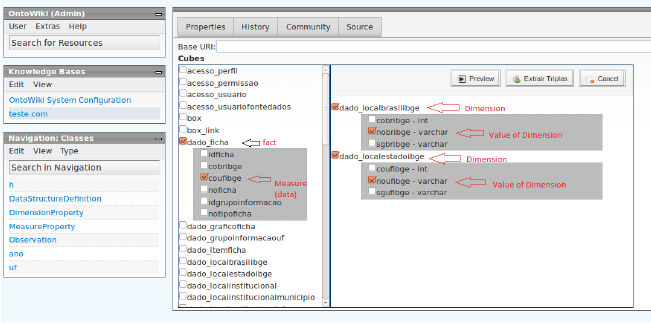
\includegraphics[width=140mm]{img/olapimport.png}
	\caption{OLAP2DataCube mapping specification example (taken from~\cite{olap2dc-paper})}
	\label{fig:olap2dc-screen}
\end{figure}

\begin{sloppypar}
That is~why the~authors introduced some steps where the~user is~asked to~do~the~following:
\begin{itemize}
  \item Select the~fact table.
  \item Select dimensions tables.
  \item Enter additional metadata --- units, description, etc. or~point to~a~  special dimension table containing the~metadata.
\end{itemize}

The whole process of~dataset conversion from relational database into~Data Cube Vocabulary
(the authors call it~triplification) is~then divided into~the~following steps:
\begin{itemize}
  \item \emph{Metadata extraction and~Table categorization} (PKs and~FKs analysis). The~  tables are precategorized as~dimension or~fact tables based on~the~number and~  direction of~FKs.
  \item \emph{Cube definition} done by~the~user as~described in~the~previous paragraph.
  \item \emph{Mapping}. The~relational database is~converted into~a~Data Cube 
  Vocabulary compliant dataset while executing a~set of~SQL queries assembled 
  based on~the~previous steps.
\end{itemize}
\end{sloppypar}

As a~matter of~fact, this process has two different outcomes. A~converted 
dataset itself and~a~definition of~dimensions. This varies a~lot from what 
we would like to~achieve. We~are about to~propose a~system, which will convert a~dataset in~order to~comply with an~already existing datastructure definition.

The authors have proven the~system qualities by~converting a~dataset of~Brasilian government data
into more than 31M triples, which is~quite a~large dataset. The~faceted browsing
capability fully depends on~the~OntoWiki platform features.

\section{Tabels}
\label{rw:tabels}
Tabels~\cite{tabels-web} is~quite an~interesting tool, which enables the~user to~convert arbitrary data into~the~Data Cube Vocabulary compliant format. 
Moreover, it~allows the~user to~interconnect the~data with its existing RDF 
representation, if~available.

The most interesting feature of~the~tool is~that it~supports a~large variety of~input types. The~user can pass a~URL of~an~arbitrary website or~upload a~file 
in many supported formats. The~application then generates an~automated script, which converts the~source document from the~input format 
into the~RDF while utilizing the~Data Cube Vocabulary standard.

Let us~imagine a~case of~converting a~webpage. The~tool parses the~source code of~the~webpage and~finds tables contained in~the~body of~the~page. Those are converted into~a~simple
RDF dataset. The~same is~done not only in~the~case of~a~webpage, but also in~a~case
of other specific supported file formats. To~achieve that a~specific algorithm is~used to~extract
the data from the~file into~a~RDF graph. After this step is~complete, the~tool generates a~DCV
datastructure definition in~respect to~the~kind of~data found in~the~input dataset.
Also, an~automatic conversion script, which the~user can later execute in~order to~triplificate
the input data, is~generated.

The script is~written in~a~custom DSL (an example in~Figure~\ref{fig:tabels}) which,
with its structure, resembles the~well--known
transformation language XQuery. Although the~script makes its job, the~user may need to~edit the~script to~improve the~behaviour. That is~one of~the~most problematic features of~this tool. The~user needs to~have a~heavy programmatic 
background in~order to~be~able to~use the~advantages of~all of~the~offered features. 
Even when binding the~data in~the~input dataset with entities in~an~existing RDF 
dataset, the~user needs to~alter the~generated script and~specify, which field 
to bind and, of~course, how.

\begin{figure}
	\centering
	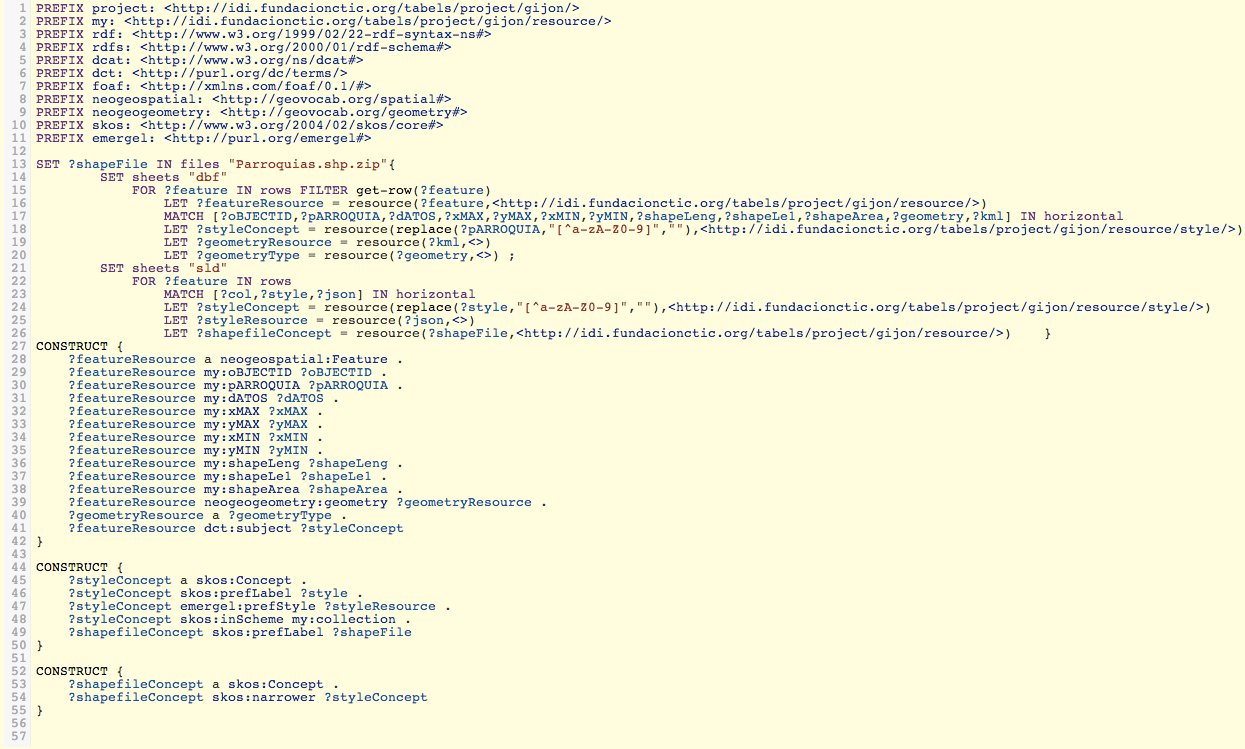
\includegraphics[width=140mm]{img/tabels.png}
	\caption{Tabels DSL example (script taken from examples repository~\cite{tabels-web})}
	\label{fig:tabels}
\end{figure}

On the~other hand, the~tool provides a~unique form of~making the~user's own Data Cube 
Vocabulary dataset based on~their statistical data in~common file formats such as~CSV, XLS, PX, KML and~formats published by~rather large institutions like Eurostat. 
The application is~therefore able to~visualize data in~charts as~well as~on~map 
in case of~geospatial data.

Moreover, the~tool also supports RDF as~an~input format, which makes it~a~competitor of~the~system we~are about to~propose. That is~why we~wanted
to~examine this tool a~bit more in~the~manner of~processing different RDF 
datasets. Despite the~fact that the~tool should be~able to~process RDF 
datasets, it~produced an~empty conversion script even on~DCV datasets downloaded 
from the~tool itself. Therefore, the~only form of~converting the~input file into~the~DCV compliant dataset was to~write the~whole script manually, while 
specifying a~set of~SPARQL construct statements. That is, in~fact, a~default 
behaviour of~any~available SPARQL endpoint, which enables it~to~execute a~SPARQL 
query on~datasets.

\section{CubeViz}
\label{cubeviz}
The CubeViz~\cite{cubeviz} tool has been developed by~the~AKSW~\cite{aksw} group
in the~scope of~the~LOD2,
a~large--scale project co--funded by~European Commission that~is~focused on~integrating and~syndicating Linked Data with existing applications.

The motivation behind this tool was to~bring a~better user--experience into~a~large--scale application, developed by~this group, called the~\emph{Open Data Portal of~European Commision}. While utilizing the~Data Cube Vocabulary standard, they 
prepared a~library of~5700 visualized statistical datasets.

\begin{sloppypar}
As well as~the~OLAP2DataCube tool, the~CubeViz is~also based on~the~\mbox{OntoWiki}~\cite{ontowiki}
application. In~fact, it~adds another layer to~the~technology stack and~provides a~way of~exploring and~discovering statistical 
data in~a~faceted browser. The~GUI is~made with common technologies like PHP,
HTML and~JavaScript. They used the~HighCharts~\cite{highcharts} library in
order to~provide data visualization (an example can be~seen in~Figure~\ref{fig:cubeviz}).
\end{sloppypar}

\begin{figure}
	\centering
	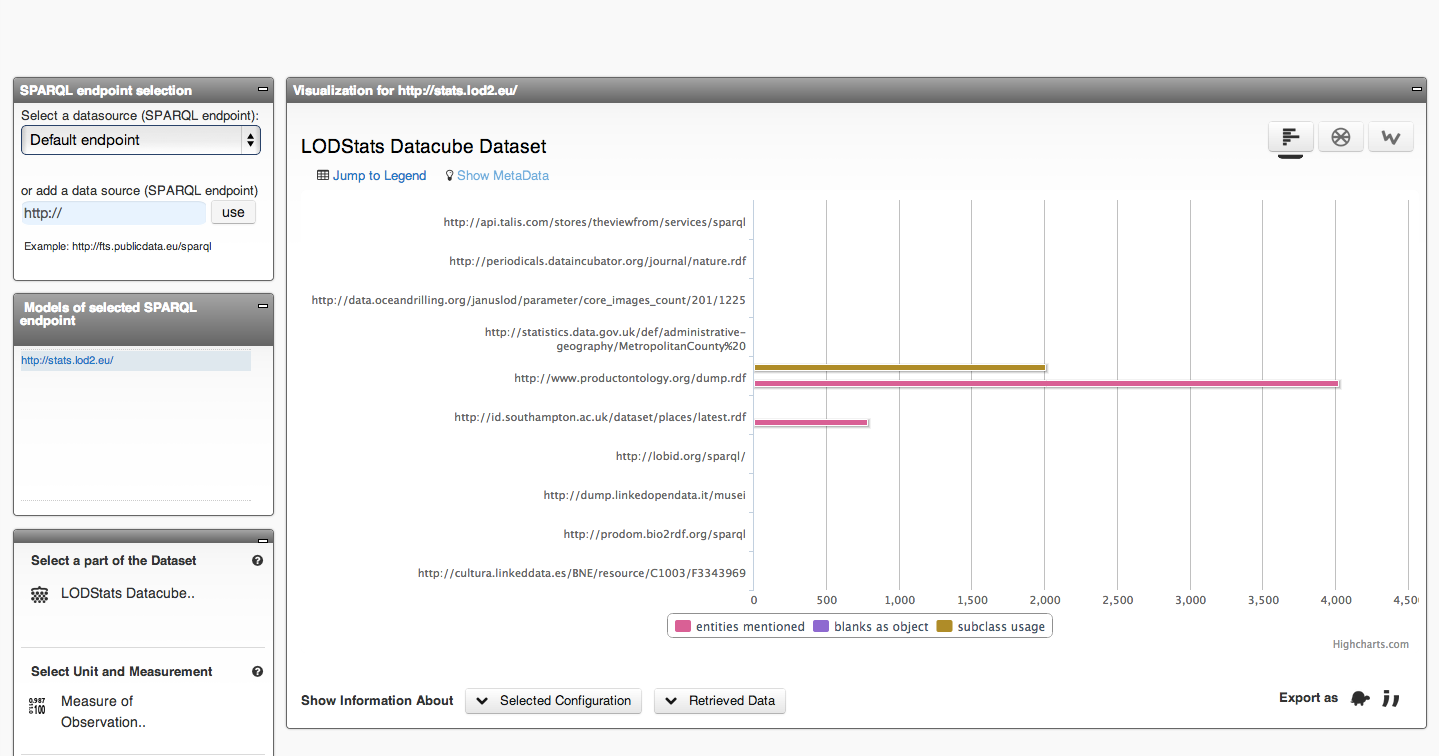
\includegraphics[width=140mm]{img/cubeviz.png}
	\caption{CubeViz visualization example}
	\label{fig:cubeviz}
\end{figure}

While utilizing the~principles of~Linked Data and~Data Cube Vocabulary 
standard, the~authors were able to~come up~with a~really sophisticated faceted 
browser, which makes the~user capable to~filter data in~detail based on~the~statistical 
semantics (DCV). The~user is~able to~filter data based on~each dimension, or~to~use the~proper term, to~slice the~cube as~needed. That gives us~a~generic tool, which 
compares any~statistical data with the~ability to~learn more 
information while taking advantage of~the~entities Linked Data interconnection.

At the~time of~writing this thesis, the~tool was limited~\cite{cubeviz-paper-1},~\cite{cubeviz-paper} to~basic chart types
such as~line, bar and~pie chart (for datasets with one dimension). Those types 
were available also for the~2--dimensional datasets for which the~polar 
chart is~offered as~well. More than two dimensions were not supported at~all. In~order to~visualize 
multidimensional datasets one needs to~slice it~into~a~2--or--less--dimensional one.
The tool also makes it~able to~publish dataset metadata.

An interesting feature of~the~faceted browser is~that the~user can 
generate a~permalink in~order to~obtain a~reference to~the~current visualization 
state. That makes it~very easy for the~user to~share their visualization with the~community.

\section{Visualbox}
Based on~LODSPeaKr~\cite{lodspeakr}, a~tool, which makes it~easier to~create Linked Data Websites 
and to~publish RDF datasets, a~visualization tool named Visualbox~\cite{visualbox} has been 
introduced. The~motivation behind this was very similiar to~those behind 
OLAP2DataCube, ViDaX or~CubeViz. The~author wanted to~present a~visual tool,
which would 
make it~easy for the~user to~understand results of~a~data analysis.

The main argument is~e.g. that a~line chart is~much more expressive and~much easier
to understand than a~table of~data or~some even more complicated data 
representation. Therefore, the~author wanted to~utilize existing visualization 
techniques people are used to~intercept.

As a~result of~this effort, he~presented~\cite{visualbox-paper} a~developer tool, which enables an~easier preparation
of a~visualization. One needs to~know basic web development technologies 
in order to~be~able to~use the~tool. Specifically, the~HTML language, the~handlebars templating syntax and~a~concept of~filters, which resembles the~concept used in~the~JavaScript MVC framework AngularJS~\cite{angularjs}. One is~however required
to posses the~knowledge of~the~SPARQL in~order to~select data and~prepare them for the~visualization. An~example of~a~SPARQL query and~a~visualization embed into~a~webpage can be~seen
in Figure~\ref{visualbox-example}.

\begin{figure}
\scriptsize\begin{verbatim}

PREFIX conversion: <http://purl.org/twc/vocab/conversion/>
SELECT ?g sum( ?triples ) as~?estimated_triples
WHERE {
  GRAPH ?g  {
   ?g void:subset ?subdataset .
   ?subdataset conversion:num_triples ?triples .
  }
} 
GROUP BY~?g

{{models.logd.triples|GoogleVizColumnChart:"g,estimated_triples,width=1200"}}
\end{verbatim}\normalsize
\caption{Visualbox scripting examples}
\label{visualbox-example}
\end{figure}

On the~other side, for those, who have this technological background the~tool is~really easy to~use. By~using a~simple snippet, the~developer is~able to~embed a~chart visualization on~the~web.

The main benefit of~this tool is~that it~brings a~unified approach to~visualising tabular data. Furthermore, it~comes up~with an~informal standard of~processing such data and~visualising them. Based on~the~Google Charts visualization 
API, it~allows the~developer to~visualize their data in~basic charts 
as well as~in~a~map if~geospatial data are present. Although the~features of~the~tool are mainly shown while visualising statistical data, the~tool has no~support for 
Data Cube Vocabulary.

\section{GeoGlobe}
The GeoGlobe mashup~\cite{geoglobe} is~an~example of~a~faceted browser for 
statistical data related to~all the~countries in~the~world. As~the~SPARQL 
query, visualization rules and~more are hardcoded in~this single--file 
demonstration, it~serves us~only as~a~great example of~what could be~the~result of~a
Data Cube Vocabulary dataset visualization.

The tool fires a~XHR request to~the~server, which contains a~SPARQL query. The~query is~executed in~order to~obtain data from a~remote SPARQL endpoint. In~fact, it~uses some Data Cube Vocabulary constructs to~filter the~data. The~data 
are sent back to~the~client in~a~form of~a~JSON string. The~mashup then uses the~D3~\cite{d3} visualization library in~order to~present the~user with a~D3 Geo 
visualization of~the~obtained data.

\begin{figure}
	\centering
	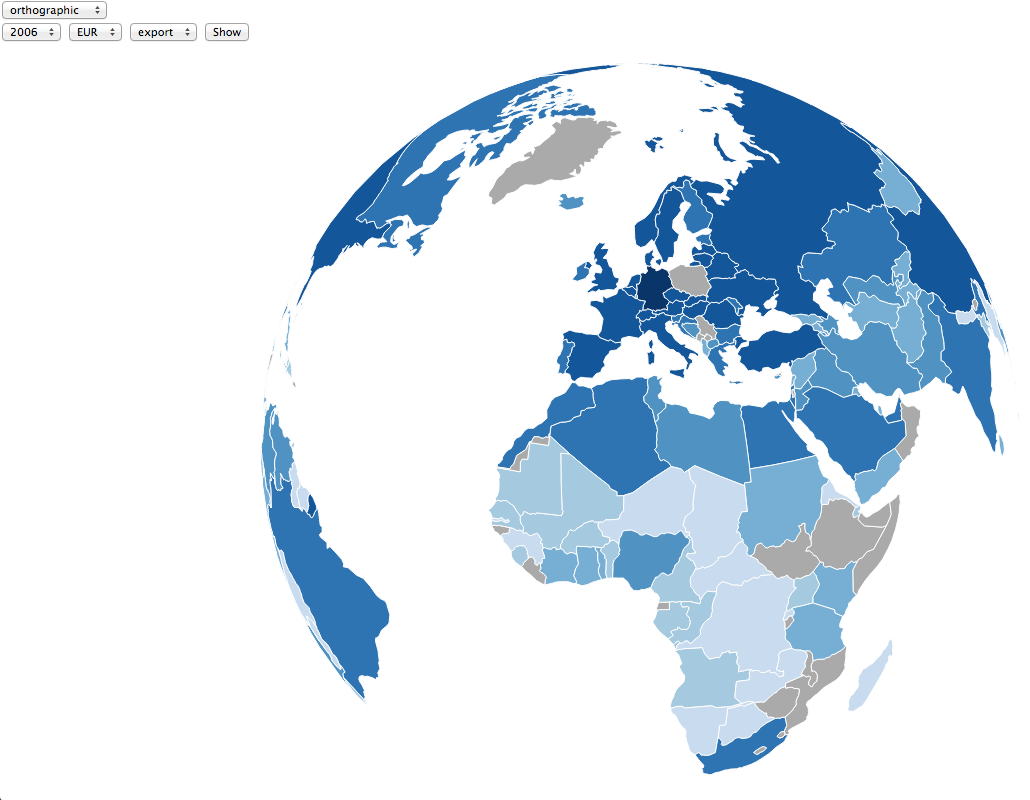
\includegraphics[width=140mm]{img/geoglobe.png}
	\caption{GeoGlobe visualization example}
	\label{fig:geoglobe}
\end{figure}


Simple GUI of~the~faceted browser changes the~contents of~the~exectued SPARQL query. 
It decides how the~original data cube is~sliced to~be~visualized as~the~user 
wanted.

\section{ViDaX}
ViDaX~\cite{vidax} is~a~desktop application written in~the~Java programming language. Based on~the~features
of the~underlying visualization toolkit Prefuse~\cite{prefuse}, it~manages to~visualize RDF data in~many ways. The~toolkit is~perfectly capable of~visualising statistical data, but the~application does not take advantage of~the~Data Cube Vocabulary standard.

Despite this, the~application has some features related to~statistical 
data. The~visualization type is~selected automatically based on~the~semantics of~the~visualized data. The~application analyzes and~normalizes the~data selected by~the~user 
and extracts the~types of~the~different properties. Those are consequently mapped to~some basic supertypes such as~Time, Location, etc. Based on~the~mapping,
the~tool offers a~visualization template to~the~user.

As a~result, the~authors presented a~tool capable of~visualizing 
statistical data with appropriate visualization type without the~need of~using 
the~Data Cube Vocabulary standard. On~the~other hand, if~the~tool 
implemented the~standard, the~results could be~even more reliable.

\section{Tabulator}
\label{sec:rw:tabulator}
Tabulator is~a~generic RDF browser and~editor. The~motivation behind this~tool
is to~provide a~generic semantic browser with serendipitous re--use. The~authors 
want to~provide a~form of~finding more relevant datasets while exploring or~publishing another datasets. 

The experimental version of~the~tool was, according to~~\cite{tabulator-paper}, 
developed completely as~a~client--side application for a~web browser. Therefore, 
technologies like JavaScript, XHR, XML, RDF and~SPARQL were utilized.

The tool offers two basic modes, exploration and~analysis. In~the~exploration mode,
the~user starts to~explore the~Semantic Web by~entering a~URI of~a~resource. They 
are then presented with a~tree view where each node represents a~resource. 
By clicking the~node, the~user expands a~subtree to~obtain more information.
The tool implicitly follows links that may contain more relevant nodes.

In order to~switch to~the~analysis mode, the~user selects fields to~define a~pattern, which is~then matched against the~original graph. The~tool executes a~specific SPARQL query to~find all occurrences of~the~selected pattern. The~projection of~this kind of~analysis could be~visualized in~many different 
views such as~a~table, a~timeline, a~calendar and~a~map. The~user can switch back to~the~exploration mode by~double--clicking on~an~instance in~the~analysis view.

The most important feature of~this tool is~an~implementation of~a~\emph{query--by--example} principle. By~highlighting the~properties in~a~tree view, the~user 
unknowingly constructs a~SPARQL query. As~a~result of~such a~process, the~user may create a~SPARQL query, which selects e.g., 
latitude and~longitude. Dataset containing such properties (geospatial data)
is then visualized on~a~map. Although the~tool is~able to~visualize statistical 
data, the~Data Cube Vocabulary standard is~not used.


\begin{figure}
	\centering
	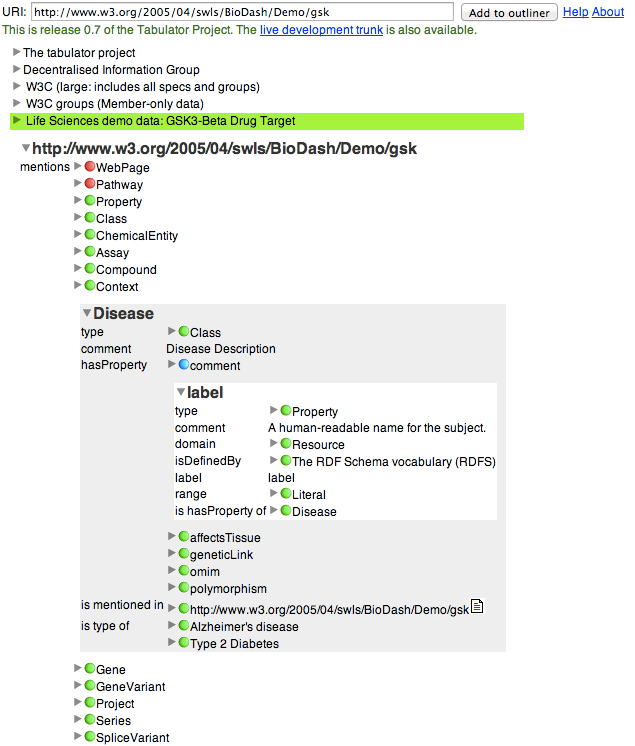
\includegraphics[width=100mm]{img/tabulator.png}
	\caption{Tabulator browsing mode example}
	\label{fig:tabulator}
\end{figure}


\section{Explorator}
\label{sec:rw:explorator}
The authors of~the~Explorator application had the~same motivation as~the~authors 
of the~Tabulator --- to~come up~with a~tool that simplifies a~dataset 
exploration. One can browse RDF datasets without a~deep knowledge of~the~RDF standard.
In order to~offer the~exploratory search~\cite{exploratory-search} feature, the~authors also
utilized the~query--by--example principle. Only simple so--called \emph{SPO SPARQL 
queries} (\texttt{SELECT \{ ?s ?p ?o \} WHERE \{ ?s ?p ?o \} }) are supported. Generally, the~tool 
enables the~user to~specify a~much simpler pattern than the~Tabulator 
application. On~the~other hand, it~offers a~faceted browser, which generates 
those queries.

Unlike the~Tabulator project, based on~information presented in~\cite{explorator},
the~Explorator is~not able to~offer any~advanced visualizations, such as~a~map or~a~chart. To~speed up~the~application, the~authors integrated a~local SESAME~\cite{sesame} 
repository where dereferenced URIs are stored.

\section{Exhibit}
The MIT Simile project~\cite{mit-simile} has spent a~more than a~decade
developing and~experimenting with software tools for Web--based data publishing.
As a~result of~the~whole process a~new tool, Exhibit, was introduced.

Exhibit is~a~JavaScript library, which produces embeddable widgets. A~developer can
easily embed a~visualization of~a~RDF dataset in~an~arbitrary web page. The~idea behind 
the~tool is~very similar to~the~idea behind the~Visualbox project. After a~quick 
examination, the~use of~the~tool is~no~more complicated compared to~the~Visualbox despite the~fact that the~manual suggests so. As~an~example of~a~visualization, we~can mention timeline, lenses and~maps. Again, the~tool is~able 
to visualize data, which could be~considered statistical, but it~lacks the~support of~the~Data Cube Vocabulary standard.

The tool became very popular for its rather easy--to--use 
approach of~publishing visualizations. The~very first version of~the~software
was introduced while completely ignoring the~problem of~large datasets.
Since it~runs in~a~web browser, it~needs to~have the~visualized data
fitted into~the~memory of~the~client 
computer. That is~why U.S. Library of~Congress initially funded the~project to~make its~authors solve the~scaling problem.

According to~the~information in~\cite{exhibit}
the~last version of~the~software supports $1000$ times more items in~the
dataset ($100 000$ vs. $1000$) and~up~to~$20 000$ properties in~the~faceted browser. 
The user is~able to~share views on~the~data after applying filters of~the~faceted browser. 

\section{Sgvizler}
The Sgvizler project is, as~the~name suggests, focused on~data visualization. 
It~is~a~JavaScript library, which parses an~HTML source and~finds specific 
element attributes. It~fills matched elements with a~data visualization based on~the~rules specified in~the~element attributes.

The developer is~required to~specify a~SPARQL query as~one of~those attributes. The~query is~executed against a~defined SPARQL endpoint. By~setting an~attribute of
the~placeholder element, the~user also specifies the~type of~visualization, which 
should be~applied on~results of~the~SPARQL query execution.

As well as~the~aforementioned tools, Sgvizler is~also capable of~visualising statistical data, 
but the~Data Cube Vocabulary standard is~not used in~any~way. For instance, in~the~case of~a~map visualization, the~library expects the~query to~return a~table 
with a~location name in~the~first column and~a~measurement value in~the~second 
one. It~does not really take advantage of~the~semantical properties in~the~dataset.

\section{Rhizomer}
Another tool focused on~faceted browsing is~Rhizomer. It~is~a~web application 
offering quite an~interesting feature, which partially fits into~the~LDVM 
concept. Based on~data filtered by~the~faceted browser, the~user is~hinted about
which visualizers are available. Moreover, 
it indicates how many entities of~the~current view will be~displayed after 
switching to~the~more advanced browsing mode.

As usually, those advanced modes are a~timeline, a~map and~a~chart visualization. As~in~the~previous cases, the~tool also works with datasets that could be~classified as~statistical, but it~does not comply with the~DCV standard. On~the~other hand, it~relies on~semantics of~the~data and~autodetects properties, 
which can have a~dimensional meaning, e.g. latitude and~longitude for geospatial data.

\section{LODStats}
The authors of~the~LODStats project suggested that a~major 
problem while working with data on~the~Web is~to~get a~clear picture of~the~structure of~a~dataset. They also introduced a~term \emph{external coherence},
which explaines how well the~resources of~the~examined dataset are connected with 
other resources, generally speaking, how the~dataset is~interconnected with 
other datasets.

In order to~solve the~problem, they have introduced the~LODStats project, an~extensible framework optimized to~work on~a~rather large datasets. Its purpose 
is to~compute statistics on~the~given datasets. The~tool is~integrated with the~CKAN~\cite{ckan} dataset metadata registry (The Data Hub~\cite{thedatahub})
in order to~cover the~most known and~most used datasets, therefore to~offer statistics for a~great part of~the~Data 
Web.

Since one can overview rather small datasets without any~significant problem, 
the~biggest advantage of~the~LODStats tool lies in~the~ability to~work fast with 
datasets containing millions of~triples of~RDF data. The~authors took advantage 
of the~presence of~a~SPARQL endpoint, which allows them to~work with the~datasets 
dynamically, without the~need to~load all those millions of~triples into~the~memory.


\begin{figure}
	\centering
	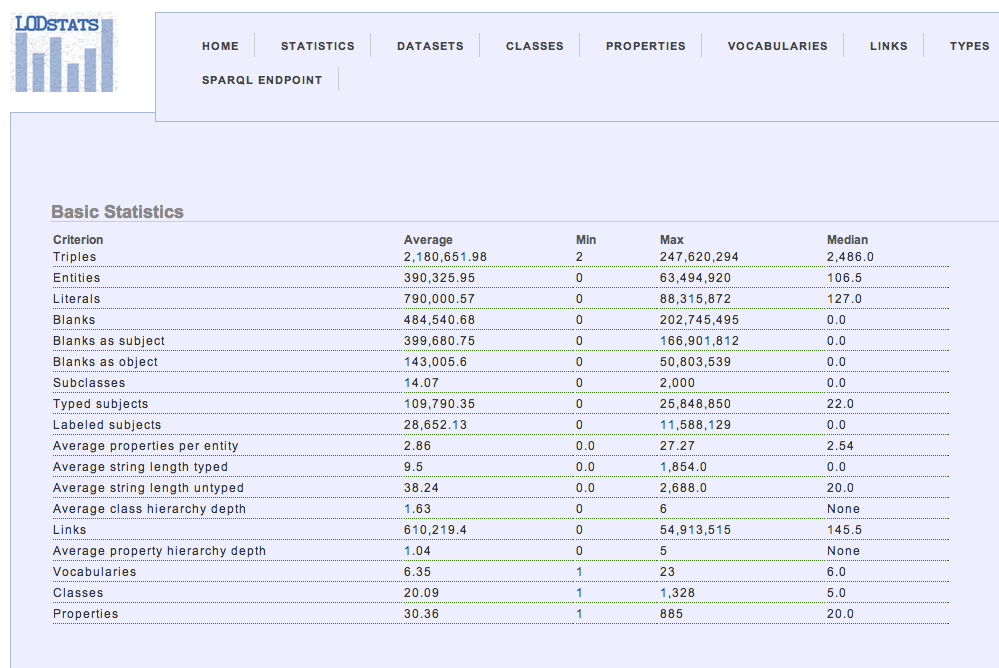
\includegraphics[width=140mm]{img/lodstats.png}
	\caption{LodStats statistics example}
	\label{fig:lodstats}
\end{figure}

The way of~processing a~dataset with a~large amount of~triples is~an~approach 
which Payola should definitely adopt in~the~future.

The authors of~the~tool implemented statistics that were defined by~VoID~\cite{void}. Which 
means that 32 different statistics are computed while utilizing the~following 
approaches:

\begin{itemize}
  \item \emph{Quality analysis} --- The~problem of~a~dataset quality is~tightly connected 
  to~the~form of~the~eventual data use. Therefore, a~static analysis should 
  give us~a~general purpose measure (similar to~Google's Page Rank) to~determine the~  quality very briefly, e.g. based on~the~number of~outgoing and~incoming 
  edges.
  
  \item \emph{Coverage analysis} --- The~authors present two subtypes of~  coverage - \emph{vertical} and~\emph{horizontal}.  While the~horizontal is~  introduced to~determine the~size of~the~domain (how many resources are described),
  the~vertical deals with the~scale of~details (how deeply the~description goes).
  
  \item \emph{Privacy analysis} --- While analyzing what classes and~properties 
  are used, the~authors of~the~project try to~determine if~a~dataset 
  might contain any~personal information.
  
  \item \emph{Link target identification} --- According to~the~authors, less than 
  10 \% of~entities on~the~Data Web are interlinked. This technique 
  should help the~user determine what dataset should the~examined one be~  connected with.
\end{itemize}

Since the~authors have focused on~performance and~declared to~develop a~tool with a~smaller memory footprint and~better scalability, it~would be~really useful to~integrate such a~tool with the~Payola tool.
The integration would give the~Payola user the~opportunity to~get familiar with the~chosen dataset before analyzing it. In~fact, as~a~circumstantial goal of~this 
thesis, we~will integrate the~tool (on HTTP communication basis) with the~previously mentioned 
LODvisualization application, the~illustration of~the~concept introduced 
in~\cite{ldvm}. Integrating Payola with the~LODStats analyzer should be~also 
possible since the~source code of~both tools is~available on~GitHub~\cite{github-payola} 
~\cite{github-lodstats}, but that is~not a~part of~this thesis.

The authors made the~tool to~examine a~given dataset in~two ways, to~examine 
the~\emph{schema-level characteristics} and~\emph{data--level characteristics}. 
The former describes the~characteristics of~an~entity in~the~context of~the~used 
schema fragments (e.g. depth in~a~tree where hierarchical ontologies are used). 
The latter then describes the~characteristics related directly to~the~values 
appearing in~the~dataset (such as~minimum, maximum values, average values, entities equality, 
etc.). An~example of~computed statistics can be~seen in~Figure~\ref{fig:lodstats}.

One will learn very quickly that Payola and~LODStats are focused each 
on something completely different, but can complement each other very well. The~Payola 
tool should definitely learn from the~statement--stream--based approach in~order 
to handle larger datasets better. The~authors of~the~tool also published
some statistics~\cite{lodstats} gathered while integrating with the~CKAN database, which is~a~great source of~information when trying to~get the~idea of~how an~average dataset 
could look like. 

\section{Yahoo Pipes, DERI pipes}
There are many analytical tools for processing RDF data. We~would like to~compare the~Payola tool with the~most important of~them and~provide the~most significant 
differences. When deciding how the~Payola tool should work, we~came 
across an~existing tool --- Yahoo 
Pipes~\cite{yahoo-pipes}. Providing an~interactive 
editor, it~allows the~user to~construct his own analytical \emph{pipe}, 
which, in~fact, corresponds with the~term \emph{analyser} (as defined in~LDVM~\cite{ldvm}).
The only exception is~that the~various offered data sources are
providing plain XML data (they are not in~the~RDF format).
The tool does not offer the~same level of~analyzing data.
It~would be~very hard to~simulate SPARQL with tools like XPath.

That is~how we~came up~with the~idea of~\emph{analyses} concept for Payola. 
We offered a~basic editor, which enables the~user to~build his own analysis
(also called an~\emph{analytical pipeline}).
 
On purpose we~made the~editor with a~rather restrictive behavior in~order to~avoid creating invalid or~incomplete analyses. The~user is~able to~insert new 
plugins into~an~existing analysis (analytical pipeline) only by~connecting it~to~an~output of~another 
one. Since we~are analyzing RDF data, the~basic set of~plugins is~strongly 
related to~the~capabilities of~the~SPARQL.

After a~while, we~came across the~DERI Pipes 
project~\cite{deri-pipes}, which is~also inspired by~the~Yahoo 
Pipes project and~is~focused on~processing RDF data. The~editor is~distributed 
in a~form of~a~Java JAR package, therefore, one should be~able to~integrate it~in~another
Java--based software rather easily.

Unlike Payola, it~contains some basic text operators, which even enables the~user  
to construct the~URL that is~used as~a~parameter of~the~RDF data fetcher. This 
is also the~biggest difference between DERI Pipes and~Payola: Payola lets 
you work only with RDF data which is~the~reason why plugin parameters (with basic data types string,
boolean, integer and~float) could not be~computed in~the~process and~are 
statically given by~the~user when defining an~analytical pipeline.

\begin{figure}
	\centering
	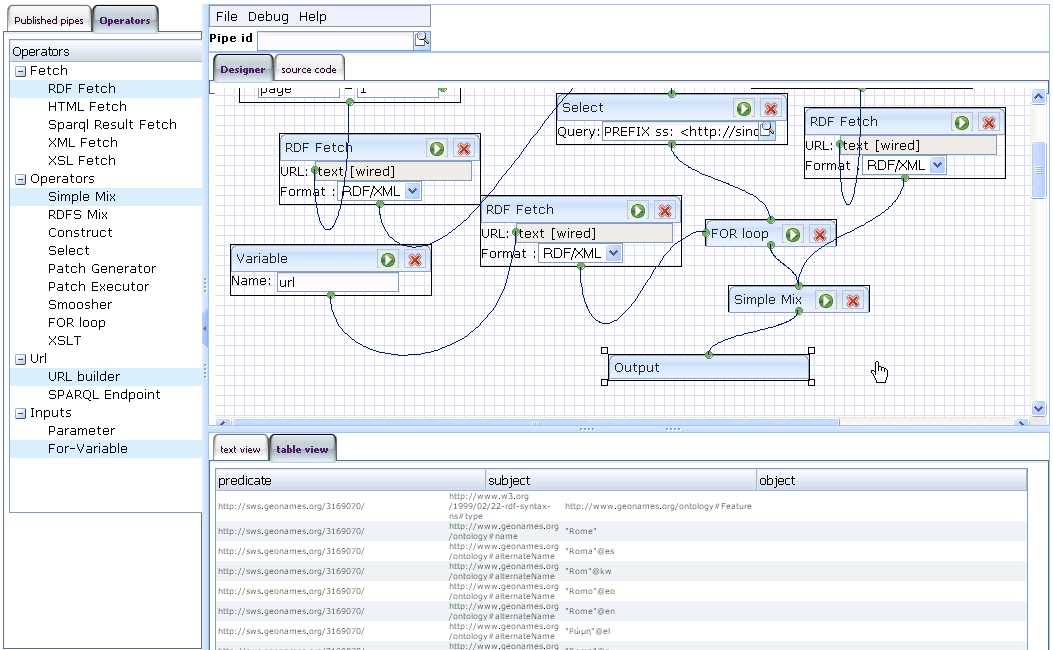
\includegraphics[width=140mm]{img/deri.png}
	\caption{Deri Pipes example as~shown in~an~instruction videocast~\cite{deri-screen-source}}
	\label{fig:deri}
\end{figure}

The DERI Pipes tool offers some of~the~operators provided also by~Payola. Some 
of them require the~user to~know the~SPARQL in~order to~fill in~the~parameters, e.g. the~\texttt{SELECT} operator. One may also apply XSLT 
transformation operators and~use \texttt{FOR} loops. It~also enables the~user to~use more datatypes as~an~input 
of a~pipe, for instance a~classic HTML document.

\section{Payola visualization model vs. LDVM}
\label{sec:rw:ldvm}
The primal reason of~the~Payola tool implementation was to~prove some basic concepts:

\begin{itemize}
\item Generic Linked Data analysis with a~web application.
\item Generic visualization of~analyses results.
\item All--in--one (read, share, analyze, visualize) Linked Data tool.
\end{itemize}

As the~original intent of~the~tool was not to~implement any~specific existing visualization model,
the~system has been created with its own internal visualization pipeline architecture. Let us~compare such
an~architecture with the~model proposed in~\cite{ldvm}. For an~easier orientation, let us~name the~Payola visualization 
model as~a~\emph{Payola model}. The~model proposed in~\cite{ldvm} is~named \emph{LDVM}. We~will describe the~Payola
model while utilizing the~terms used in~\cite{ldvm}. Moreover, we~will also explain
the~differences between the~LDVM and~the~Payola model.

The Payola system is~able to~visualize all kinds of~RDF data. It~retrieves them from different
types of~RDF storages. Since it~is~not currently important, suffice it~to~say that it~just fetches
arbitrary RDF raw data. It~uses SPARQL \texttt{CONSTRUCT} queries to~retrieve those data from
the~given sources in~order to~work with graphs.

After the~dataset is~fetched, it~is~processed by~an~\emph{analyzer}. This could be~a~set of~any~kind
of transformations or~operations. The~most common case is~running a~SPARQL query
on the~input graph. The~only invariant is~that the~analyzer retrieves a~RDF graph
representation and~its output is~also a~RDF graph representation (regardless of~a~concrete
implementation). This is~the~phase described in~\cite{ldvm} as~\emph{Data transformation}.
Naturally, the~product of~such an~operation is~a~result of~the~analysis, which is~called an
\emph{Analytical abstraction} in~\cite{ldvm}.

\begin{sloppypar}
Since Payola is~a~web application, which delegates rendering the~view to~the~client--side
of the~application, the~result of~an~analysis is~transformed into~a~simplified format for a~\emph{visualizer}.
At first, the~result, which is~an~RDF format representation, is~serialized to~a~custom \texttt{JSON} string
that is~transferred to~the~client--side. The~string is~then deserialized to~an~internal visualizer
representation. In~fact, this procedure is~similar to~one called \emph{visualization transformation}
in~\cite{ldvm}. The~product is~the~\emph{visual abstraction}~\cite{ldvm}.
\end{sloppypar}

When the~visualizer has all the~data it~needs, it~maps the~visualization abstraction to~a~visual
representation, or, as~described in~\cite{ldvm}, to~a~View. Actually, the~process of~mapping in~\cite{ldvm}
described as~Visual mapping transformation is~just traversing the~retrieved data and~interpreting
them in~a~visual form (regardless of~the~concrete form).

As one can see, the~Payola model and~the~LDVM are very similar. In~fact, the~Payola pipeline
architecture corresponds with the~proposed LDVM with some minor exceptions. Some of~them
originate from the~fact that the~Payola model is~the~result of~an~implementation
based on~concrete technologies. That is~why some additional constraints (especially
the~graph invariant) are added.

Another exceptions issue from the~modularity of~the~Payola system. The~system was designed
to provide a~platform, which also means that the~developer is~able to~build his own visualization 
plugins. This suggests as~well that while serializing data into~the~JSON, the~platform cannot perform
any data optimizations in~order to~preserve all available information. Let us~remind the~reader of~a~part of~visualization transformation definition from~\cite{ldvm}:

\emph{The goal of~this transformation is~to~condense the~data into~a~displayable size and~create
a~suitable data structure for particular visualizations.}

This operation may be~repeated \emph{on--the--fly} in~the~visualization mapping transformation
phase by~the~concrete visualization plugin chosen by~the~application user. In~fact, one can
say that the~visualization transformation phase is~duplicated and~the~pipeline contains two
stages of~\emph{visual abstraction}. One can see an~overview of~the~Payola 
visualization model in~the~fig.~\ref{fig:payola_model}.

\begin{figure}
	\centering
	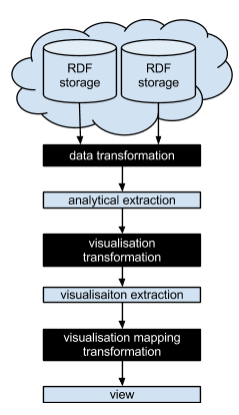
\includegraphics[width=100mm]{img/payola_model.png}
	\caption{Payola visualization model}
	\label{fig:payola_model}
\end{figure}

\subsubsection{LOD visualization}
\label{rw:lodvis}
To prove the~concept of~LDVM, one of~the~authors decided to~come up~with a~tool 
based on~the~concept. The~LOD visualization tool~\cite{lodvis} is~oriented
to perform well on~rather big datasets and~provide their main characteristics in~a~reasonable time. Its main purpose is~to~enable to~orient quickly in~a~given dataset. It~provides several 
visualization types that help the~user to~understand the~structure of~the~dataset.

That is~also the~most significant difference between the~Payola tool and~LOD 
visualization. The~basic Payola analyzer and~visualizer implementation provides 
deep details. It~shows the~whole dataset in~the~most possible detail. In~fact, 
the~performance could become an~issue on~a~rather larger dataset.

Those two tools are actually complements. While working with a~dataset one could 
start with the~LOD visualization tool to~get the~overall picture of~the~dataset --- 
the~\emph{data coherence}. It~will also help to~get the~idea of~what is~included in~the~dataset without making a~specific query.

Payola comes in~when one is~familiar with the~structure of~the~dataset. The~user 
is now able to~perform specific queries, analayze the~dataset and~attempt to~make a~visualization of~the~analysis result. Therefore, one of~the~minor tasks of~this thesis
will be~a~simple integration of~the~LODvisualization tool into~Payola.

\begin{figure}
	\centering
	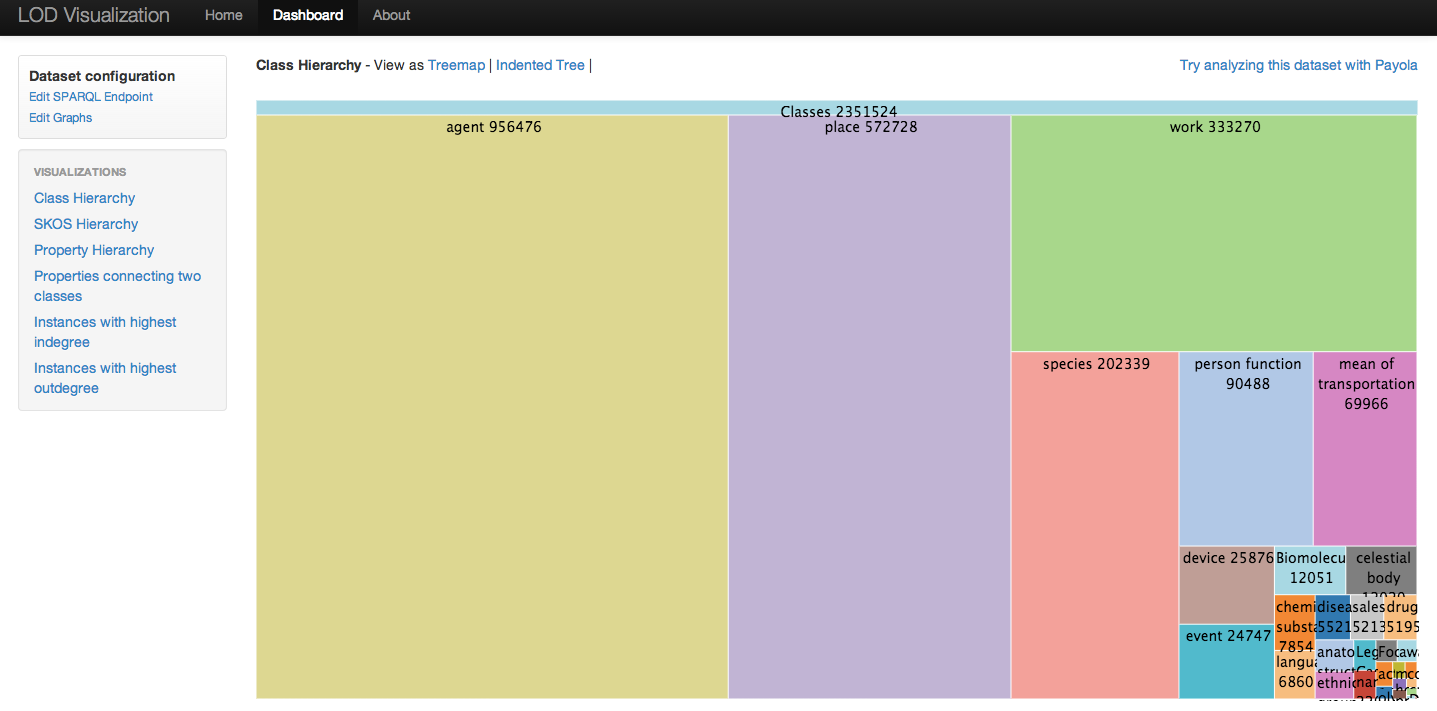
\includegraphics[width=140mm]{img/lodvis.png}
	\caption{LodVis visualization of~DBPedia class hierarchy}
	\label{fig:lodvis}
\end{figure}

The user of~the~LOD visualization tool is~able to~utilize the~following 
visualizations:

\begin{itemize}
\item Class hierarchy.
\item SKOS hierarchy.
\item Property hierarchy.
\item Properties connecting two classes.
\item Instances with the~highest indegree.
\item Instances with the~highest outdegree.
\end{itemize}

In a~form of~an~interactive treemap or~tree view, one 
can traverse through the~tree that expresses the~hierarchy of~RDF classes used 
in the~given dataset. One can also do~the~very same thing with properties. The~user is~also able to~list all of~the~properties that are somehow (in both directions)
connecting any~two classes from the~dataset. When given a~class, the~tool is~able to~quickly find an~instance of~such a~class, which is~the~most referenced
instance. It~is~also able to~determine what instances have the~largest amount of~references
--- they have the~highest amount of~outgoing
edges.

\subsubsection{The extended version of~LDVM}
Since the~original paper was published on~ISWC 2012 as~a~demo and~a
work--in--progress, the~model is~being developed even while writing the~text of~this thesis. We~will operate with the~latest available version~\cite{ldvm2} and~look 
at the~new features of~the~proposed model. In~fact, the~latest version of~the~paper also covers an~evaluation of~RDF data visualization tools including 
Payola.

The most significant change came with introducing the~concept of~a~\emph{visualisator 
reusability}. The~authors talk about so--called~\emph{GVDTs} (Generic visualization Data Types).
That forces us~to~think about what types of~visualizators we~could need. That applies also to
one of~the~core products of~this thesis --- visualizators for multi--dimensional data.
One will probably repeatedly use a~limited count of~visualizers.

While Payola makes it~possible to~reuse a~visualizer, it~does not satisfy the~requirements set down in~the~proposal~\cite{ldvm2}. The~idea goes a~little bit 
further, beyond the~borders of~a~single application. Being integrated with the~LOD cloud, it~should be~possible to~query it~with the~characteristics of~the~data we~would like to~visualize and~get a~list of~visualizers 
available in~the~cloud and~suitable for the~task.

By reusing this concept, the~same could be~applied to~analyzers and~so--called 
\emph{transformers} designed to~transform the~results of~an~analysis 
into another form more suitable for a~certain class of~visualizers. 
That could include a~process of~gathering more useful data (e.g. to~visualize 
some data on~a~map it~is~needed to~enrich the~dataset with a~GPS locations).

The result is~a~dynamic pipeline architecture (\emph{LDVM Pipeline Instance}),
starting with an~arbitrary 
dataset passed to~some analyzer followed by~a~chosen transformer ending up~with
visualising the~result with one of~the~visualizers. As~a~result of~applying the~concept,
we would obtain something similar to~dynamic 
registry of~analyzers, visualizers and~transformers.

To make the~Payola tool 
compliant with this concept, we~would need to~introduce a~module, which allows the~user
to describe the~analyzer (user--made analyses) and~make the~analyses more reusable. Currently, each analysis is~tightly connected to~the~data sources it~utilizes and~those cannot be~easily switched. That would, in~fact, require massive changes in~the~analyses editor, which is~not very 
user--friendly when it~comes to~editing an~existing analysis.

The concept of~transformers is~completely missing in~Payola since, as~stated 
before, it~is~up~to~each visualizer to~transform the~passed data into~a~more 
suitable form, even enrich them with necessary information.

All the~visualizers currently implemented in~the~Payola stack are fully 
reusable. But the~tool lacks the~feature to~receive data from an~external source 
and apply a~visualizer on~them. Or, from another point of~view, there is~no~way of~invoking the~visualizer itself and~specify where the~data is~and~execute a~visualization process.

All those missing features have one thing in~common. Payola is~missing 
an~API, which would be~able to~tell, which analyzers, transformers and~visualizers are present in~the~current installation of~the~tool and~provide a~machine--readable description of~such components. Moreover, it~is~missing a~mechanism that will allow the~user to~run those components separately out of~the~context of~the~Payola tool.

The authors call the~above a~\emph{compatibility} in~~\cite{ldvm2} and~introduce a~formalization that involves defining an~\emph{input signature}.
In case of~the~basic Payola components, with an~exception of~one visualizer, the~signatures
would be~empty. This would effectively express the~fact that they are designed to
visualize every dataset. The~only exception is~the~\emph{Chart visualization},
which requires the~data to~have a~specific pattern so~it~would be~sufficient to~sign it~just with a~SPARQL query. While speaking about analyses made by~the~user or~more 
advanced visualizers, ontologies would also come in.

\section{Payola visualisator framework features}
\label{sec:rw:mantra}
Since there are generally many publications focused on~data visualization (with no
connection to~Linked Data), we~would like to~compare the~recommended approaches to
the~implementation of~visualizers embedded in~Payola.

Ben Shneiderman in~\cite{mantra} introduces a~term \emph{Visual lnformation--Seeking Mantra}.
He tries to~define
what a~good visualizer should provide to~satisfy its user. He~also puts those definitions into
a~context with some specific data formats, more particularly with multi--dimensional data,
which are related to~the~topic of~Linked Data, moreover the~Data Cubes metaformat. We~try to
compare the~specified list of~features with those provided by~Payola. We~also want to~explain,
why some of~those features are missing or~provided in~another form.

The author states that every visualizer should have the~following features:

\begin{itemize}
\item Overview.
\item Zoom.
\item Filter.
\item Details-on-demand.
\item Relationship view.
\item User actions history.
\item Sub-collections extractions.
\end{itemize}

Let us~go~through the~list of~the~features and~comment them gradually. All the~visual plugins
embedded within Payola provides the~\emph{Overview}. It~is~important to~state
that it~contains some limitations. Since Payola is~a~generic Linked Data visualization tool,
the~output of~practically all of~the~plugins is~a~graph (network). It~contains all of~the~vertices
included in~the~visualized dataset. Those are placed by~a~given algorithm on~the~screen,
but are not clustered. The~result is~that the~user is~(in most cases) able to~see the~whole
dataset on~his screen. But the~visualization could be~a~bit confusing since all the~vertices
are present. The~recommended adjustment would be~to~somehow simplify the~initial view.

\begin{figure}
	\centering
	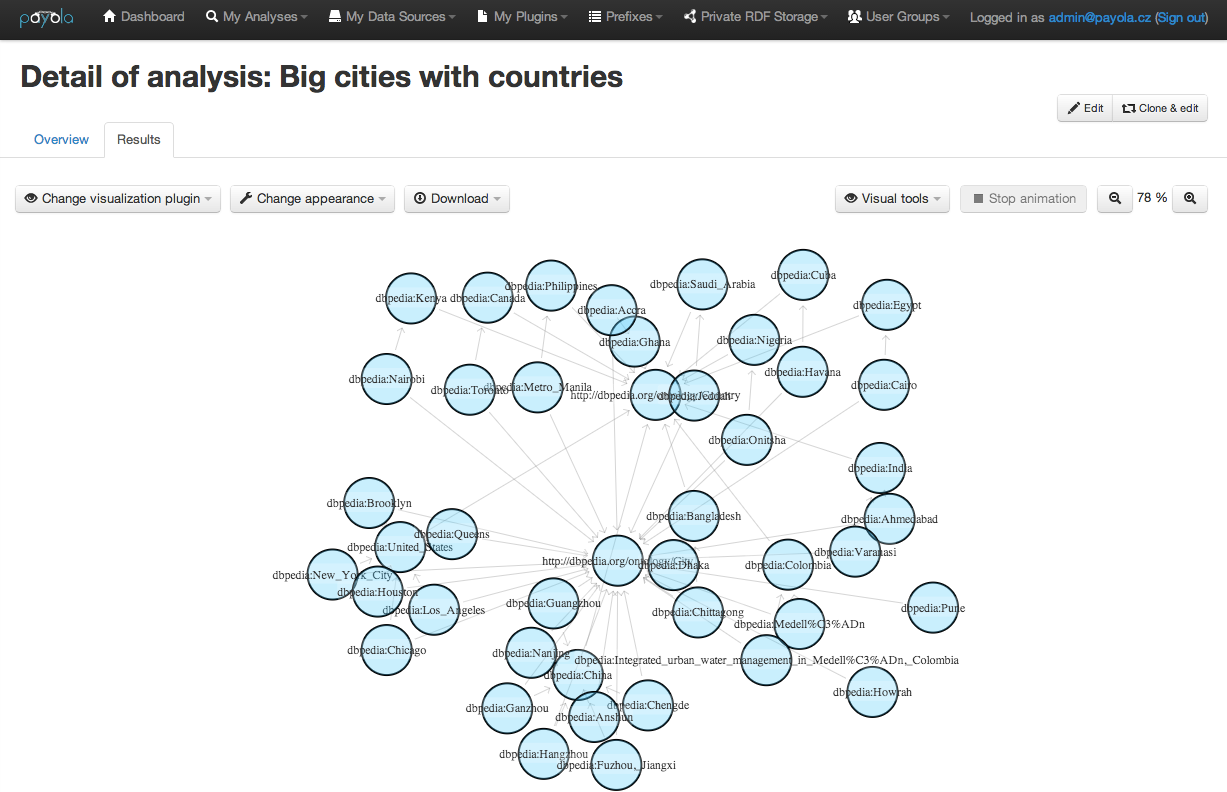
\includegraphics[width=140mm]{img/payola.png}
	\caption{Payola analysis result visualization}
	\label{fig:palyola-vis}
\end{figure}


The visualized graph might be~dense. Some of~the~used algorithms will create a~graph, which
will have virtual clusters of~vertices with a~very little distance between them. In~fact, some of~those
vertices would be~so~close to~one another that they would overlap. Therefore Payola enables the
user to~\emph{zoom} in~and~regulate the~virtual distance between vertices.

When speaking about the~\emph{Details--on--demand} feature, we~would like to~distinguish
between two different
scenarios:

\begin{itemize}
\item Detailed information about a~vertex.
\item More detailed relationship information.
\end{itemize}

To make the~view more synoptic many of~the~embedded plugins extract the~related literal
vertices and~collapse them into~a~vertex meta information. E.g. the~entity
\url{http://dbpedia.org/resource/Dhaka} has some properties - \texttt{label},
\texttt{populationDensity}, \texttt{populationTotal}.
Those are actually relations. Despite that fact, visualizers do~not treat them
that way. They store this information in~the~memory and~display it~if~and~only if~the~user
interacts with the~related vertex.

The most missing Payola feature is~loading relationships on--demand. With the~connection to~the
problem
mentioned in~the~overview section of~this chapter it~would be~more suitable, if~the~Payola system
would enable the~user to~view only significant vertices at~first and~only load details when needed.
This is~also connected to~the~\emph{Sub--collections} extractions feature, which is~partially available
in the~analytical Payola module.

Since Payola visualizes Linked Data, it~naturally visualizes the~\emph{relations between the~entities}.
The only feature, which is~rather missing in~comparison to~the~feature list from~\cite{mantra}, is
\emph{User actions history}.
There is~only one component of~Payola that enables a~user to~walk through 
history of~actions and~that is~a~SPARQL endpoint browser. It~remembers the~path 
that the~user creates while clicking through the~dataset. The~other visualizers 
however are not equipped with such a~feature.

Payola does not fulfill the~basic thought stated in~\cite{mantra}, since 
there is~no~visualization plugin that would enable the~user to~overview the~examined data set via a~specialized visualization such as~a~treemap 
in~\cite{lodvis}. What one gets after visualizing the~results of~an~analysis is~a~detailed view, which is~(in the~case of~graph visualizations) however zoomed out
to enable the~user to~see the~whole dataset at~once. Despite that fact, it~contains representation of~all the~nodes in~the~data set and~therefore breaks 
the~visual information seeking mantra.

\chapter{Payola}
\label{ch:payola}

Quite some time ago, we decided to participate on a~large--scale software 
project focused on analyzing and visualising Linked Data. As a~result of the~project
a~completely new tool, Payola, was introduced. Since we are proposing a 
system, which could fit into the technological stack of Payola, in this chapter, 
we will get the reader familiar with the tool. Even if we  decide 
not to integrate the system we are about to propose, the Payola tool remains
a related work tool and worth describing.

Payola is an~HTML5 application oriented on a generic processing of Linked Data. 
The main goal was to come up with an~application that will eventually reduce the~software 
stack one needs to browse, analyze and visualize Linked Data. We wanted the~tool 
to compile some existing approaches and bring a~compact way for processing LD.

Upon a closer look at Section ~\ref{chap:rw}, it will become apparent that many of those tools are
immensely capable. However at a more detailed look one will see that they might have to
be chained in order to convert data into 
RDF, perform analysis over an~RDF graph and visualize those results.

Payola, on the~other hand, is a~framework developed with keeping in mind that 
the user should have no need for another tool to process their data. However, as a~
large--scale project actively being developed, it still lacks many 
features and originally offers just a~basic set of operations to enable a
\emph{generic} processing of an~arbitrary dataset.

To understand the~architecture of a possibly proposed plugin, we need to walk the reader 
through the~architecture of the~framework itself. But, to be able to understand 
the architecture of the~system it is required to familiarize oneself with its features first.

\section{Payola concepts}
In order to fully understand the~following text, let us explain some concepts 
implemented in Payola:
\begin{itemize}
  \item \emph{Data Source} --- data storage with a~defined interface like a~SPARQL endpoint.
  If we talk about a~data source, we almost always have in mind an~RDF data source.
  
  \item \emph{Analysis} --- one can look at an~analysis as an~algorithm, which 
  describes working with data from a data source in order to provide results. 
  It is a~way of specifying the data sources you want to fetch the~data from, 
  filtering them, combining them, constraining them on properties, applying 
  ontologies, etc. Also known as an analytical pipeline or an analyser.  
  
  \item \emph{Plugin} --- as Payola is a~platform, it is reasonable to expect that 
  some of the~features might get to be extended by plugins. In 
  Payola, we distinguish between two different types of plugins --- \emph{analytical plugins} and 
  \emph{visualisation plugins}. Whilst visualisation plugins are small components, 
  which take an~RDF graph as an~input, the~analytical plugins are processing 
  units, which generally transform one~input graph (or more) into another one.
  
  That includes anything from a simple forwarding of the~graph from input to output, 
  making union of two graphs, executing a~SPARQL query on the~graph to constructing 
  a~completely different graph. The new graph is created by applying in--memory
  operations defined by the~source code of the~plugin.
  
  \item \emph{Data fetcher} --- a~component, which serves to fetch data from a~data 
  source. For example, while communicating with DBPedia~\cite{dbpedia},
  a~data fetcher is needed to connect to a~SPARQL Endpoint, execute a~
  SPARQL query against it and return the~results.
\end{itemize}

\section{Payola features}
Basically, we differentiate between two types of Payola users --- anonymous and registered. 
While an~anonymous user has a~very limited accessibility as they can only 
view and explore publicly available resources a~registered user is able to 
take a full advantage of the~application.

One of the~basic features offers the~possibility of creating your own instances of a~
data source. Based on the~available data fetcher types, the~user is able to create 
his own instance. An instance is a mean where one specifies parameters of a~
concrete data fetcher. For example in the~case of a~SPARQL Endpoint data fetcher,
the user fills in the~URL of the~SPARQL Endpoint and optionally a~URI of the~named graph 
containing the~desired dataset. Having done this, the~user is able to share 
such an~instance with the~other users of Payola.
Moreover, the~user can make it 
publicly available and share an~URL of that instance, which allows any 
Internet user to browse through the~data source equally as its owner.

\subsection{Exploration mode}
On the~application dashboard is the~user presented with a~list of accessible 
resources, including data sources. After clicking on a~data source the~user is
presented with a~neighbourhood of an~\emph{initial vertex}. The choice of an~initial vertex
depends on the~implementation of the~underlying data fetcher.
Those bundled with Payola choose a~random entity from the~data source
and use it as a~starting point of a~data source exploration.

The user is also provided with his own data repository, which is created by 
Payola in the~underlying installation of the~Virtuoso~\cite{virtuoso} triplestore. Payola then eases 
the upload of an~arbitrary dataset in the~RDF/XML or TTL 
format into the~private repository. The repository may be used as a~data source in analyses.

In the~exploration mode, one can choose from a~couple of visualisation plugins. 
By default, the~results are displayed in a form of a~triple table, but the~user can 
opt to more advanced modes --- a graph visualisation and a chart visualisation
(which currently requires a~special pattern to be present in the~data). By using those 
visualizers, the~user is able to traverse from a node to a node, thus exploring the~whole 
dataset.

\subsection{Analytical mode}
In the~analytical mode, the~user is able to build a~custom data analysis. As 
stated before, an~analysis could be presented as an~algorithm, which decides 
how to process data. Moreso, in the~analysis, one is expected to specify 
where the~data have to be fetched from.

The analysis concept arises from ideas seen in projects like DERI 
Pipes~\cite{deri-pipes}, meaning, that the~user is needed to assemble a~pipeline,
which processes the~input data in a~specified way. Therefore, to enable them a 
building of an~analysis, Payola is bundled with several basic 
plugins. Generally, the~list of plugins contains as many plugins as needed
in order to simulate basic SPARQL query behaviour.

\begin{itemize}
  \item \emph{Typed} --- This plugin selects vertices of an~RDF type that is filled in
  as a~parameter called RDF Type URI from its input graph.
  
  \item \emph{Property Selection} --- the~plugin takes property URIs separated by the
  newline character as a~single parameter. It selects vertices connected
  to others using one of the~listed URIs.
  
  \item \emph{Filter} --- the~plugin lets the~user select vertices with an~attribute of
  a~particular value or property.
 
  \item \emph{Ontological Filter} --- this plugin filters the~input data so that the~
  result contains only vertices and properties defined in an~ontology specified 
  by the~given URI.
  
  \item \emph{SPARQL Query} --- a~plugin for more advanced users who are capable of 
  constructing a~custom SPARQL query. Since plugins in the~pipeline work solely with 
  graphs, the~SPARQL query should be of a CONSTRUCT type.
  
  \item \emph{Union} --- a~plugin with more than one input. As the name suggests, it takes 
  the~input graphs and unifies them into a~single one that is passed onto the~
  output.
  
  \item \emph{Join} --- the~behaviour of the~Join plugin could be a~bit tricky so it is advisible
  to take a~closer look at it in the~application's 
  user guide~\cite{payola:ug:join-plugin}. The most common case simulates the~
  behaviour of the~join statement as we know it from the~world of relational 
  databases.
  
\end{itemize}

An example of an~analysis can be seen in the~figure~\ref{fig:example-analysis}.
The goal of the~analysis is to query against DBPedia SPARQL Endpoint and 
retrieve cities with a~number of population higher than the~specified parameter. 
Those cities are then connected to the~country they belong to.

\begin{figure}
	\centering
	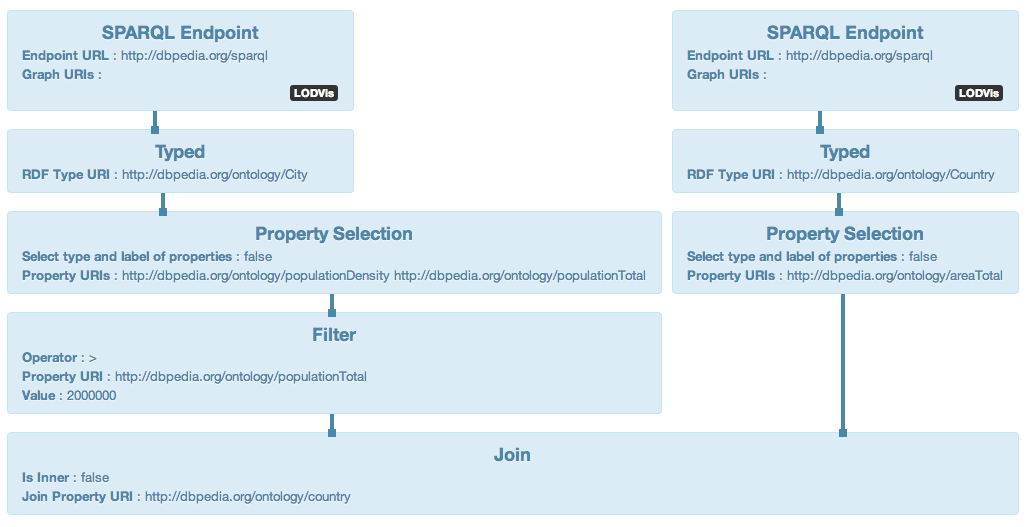
\includegraphics[width=150mm]{images/example-analysis.png}
	\caption{An example of Payola analysis}
	\label{fig:example-analysis}
\end{figure}

\subsection{Visualisations}
One would certainly like to visualize the~results of an~analysis. Therefore, 
Payola is bundled with some basic visualizer plugins. As described
in Chapter ~\ref{chap:rw}, the~Payola basic visualization 
plugins support some features suggested in the~Visualisation 
mantra~\cite{mantra}.

The bundled plugins enable the user to visualize the~results of an~analysis 
in a~couple of different ways. The basic visualisation generates a~triple 
table, while more advanced variants offer a~generic graph visualisation with a 
support of OWL ontologies. The visualizer allows the~user to customize the~
view based on an~ontology. The user can customize colours and other graphical 
features of a~rendered graph representation in respect to a~URI type defined in 
an ontology.

\subsection{Sharing}
Since Payola was designed as a~collaborative tool, it contains group 
managements and a~generic mechanism for sharing. Many types of content such as a 
data source, an analysis, a custom analytical plugin, an ontology customization for 
visualization, all can be shared with other users of the~Payola application 
installation.

Since the~description of the~tool is not the~main goal of this thesis, we will 
keep it brief and refer the reader to the~Payola User's guide~\cite{payola:ug} to learn more.

\section{Payola architecture}
The application is divided into several parts, packages, in fact. That can be 
seen in Figure~\ref{fig:packages-structure}. Since this will be useful in an upcoming
chapter about implementation, we will look at them more closely.

At first, there is the~\texttt{common} package consisted of a code, which is 
shared with all of the~other parts of the~application. Every other packages can 
access it and use the~declared code. Moreso, the~classes and objects 
in this package are automatically compiled into the~JavaScript language and are available
also on the~client--side. As an~example of a~class from the~common package, we
can name the \texttt{Graph} or \texttt{Vertex} classes, which serve as object representations
of an RDF graph or a~vertex (resource, entity). Moreover, there are traits for 
entities that are consequentially independent on a~concrete DAL implementation.

The domain package contains a~code related to the~business logic of the~
application. It solves mostly basic operations for entities, such as
\emph{add a~user into a~group} or \emph{grant a~certain privilege to a~user}.
It also contains components related to the~analytical plugins compiler. The 
compiler is executed when a~user submits their own analytical plugin via the~user 
interface. It validates and compiles the~code. If successful, the~plugin is 
loaded into the~application. Last, but not least, the~\emph{analysis evaluator} is 
present in this package. Since this is crucial, we will talk about the~evaluator
in more detail in this chapter.

The data package then wraps the~entities from the~previous packages with a
concrete implementation of DAL (Data Access Layer), which in our case is the~Squeryl
ORM framework~\cite{squeryl}.

The model package builds up a~wrapper, which encapsulates all the
business and data access logic. The goal of the~code in this package is to decouple
any presentation layer from the~application logic and data access. In fact,
all of the~existing presentation layers (web application controllers and
RPC remote objects) are built on top of this package. 

The web package contains all the~code needed to build the~web application --- 
a server side, a client--side and everything in between. It contains the~code of 
the MVC application as well as the~code of the~client--side subapplications.
It also contains the~code of visualizer plugins and an analysis editor. One of the~
most difficult and interesting features from this package is the~RPC mechanism.

The RPC mechanism was implemented in order to bridge the~gap between the~client 
side and the server side application and to hide the~XHR request from
the~developer of the~application and/or any extension. Since the~application heavily
uses the~\emph{Scala to JavaScript} component, we invested some effort into developing the~RPC 
protocol. That enables a developer to transparently call a~method on the~server from 
the client--side. 

\begin{figure}
	\centering
	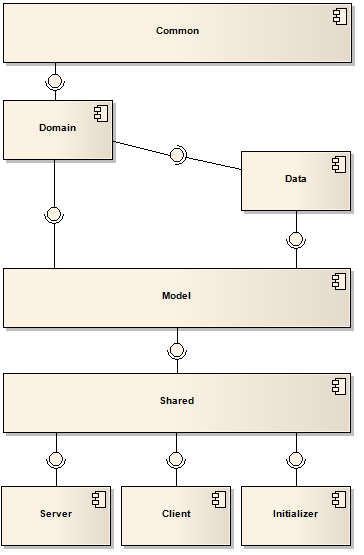
\includegraphics[width=100mm]{images/project_dependencies.png}
	\caption{Packages structure}
	\label{fig:packages-structure}
\end{figure}

To learn more about the~architecture or the implementation details, please see the~
Payola Developer's Guide~\cite{payola:dg}.

\section{Analysis evaluation}
When we are now familiar with the~parts of the~application, we may explain a~
bit more the processing and visualizing of an analytical pipeline. That is 
crucial to know before an implementation of any extension.

When an~analysis evaluation is requested, the~analysis gets \emph{validated}. We need to make
sure that the application meets some requirements, e.g. it has one 
\emph{output}, all \emph{inputs} and outputs of all the~plugins in the~analysis are \emph{bound}, etc.
If it does, the~application tries to \emph{optimize} it. Generally, executing a~plugin 
means that it is provided with an~input graph, it performs some operations and 
returns another graph. Since the~project has integrated the~Jena library~\cite{jena}, it is 
very easy to query an~in--memory representation of a~graph and return the~
results.

Let us imagine a~situation where a~user wants to select a~rather small range of 
data from a~data source. For instance, a~list of cities from DBPedia, which includes those
with a~population count higher than $2000000$ people. Without an~optimization
the evaluator would have selected all available entities from the DBPedia 
database (which is not possible anyway due to their SPARQL endpoint 
configuration). After transferring all of the~data to the~Payola server, it would have
executed a~simple SPARQL \emph{typed\&filter} query in the~memory.
However, this would be a~far cry from an~efficient solution. It would even
bring many technical difficulties, e.g. the~whole DBPedia dataset would require 
the Payola server to have a~huge amount of RAM.

That is why an~optimalization would take place in such a~situation. The original 
query which would fetch all the~data from DBPedia would be altered to include 
the constraints set by the~presence of typed and filter plugins, so that the~
data fetcher would have to fetch as less data as possible. The optimizer can 
also handle unions or joins over the~same data sources.

That gives us the~idea of how the plugins work and how they can cooperate in the~
context of analysis with optimalization. The evaluation itself is transformed 
into a~problem, which is solved by the~Scala Actors framework. For each plugin 
in the~optimized analysis, there is an~instance of an~actor. The actor waits 
until all of~the~inputs of the~corresponding plugin have been provided with the~
input data from its predecessor. When inputs are bound with input data, the~
executive part of the~plugin is performed. That could be anything from 
executing a~SPARQL query to finding the~shortest path between two nodes in a~
specified graph. The only constraint is that the~result of the~plugin execution 
needs to be also a~graph.

As the~last plugin (with no bound successor on its output) gets evaluated, the~
analysis is done. The results are sent via RPC (while being serialized into JSON) 
to the~client--side and visualized by the~basic visualisation -- the~triple 
table. The user is then able to switch to another visualisation. The JSON 
representation of the~resulting graph is stored in the~memory of the~user's web 
browser and every visualizer, which is activated by the~user accesses the~
in--memory representation and renders whatever it needs into a~given canvas.

That is a~brief description of the~evaluation process. It offers an insight
to what happens of in the~background. Later, we will learn how this affects 
the implementation of the~proposed system.

\section{Technological stack}
In order to deliver an~application, which is easy to use and does not require 
the user to install it on a~client machine, Payola is being developed as a~web
application. Since it is assumed that Linked Data community is consisted of
rather advanced computer users with modern web browsers installed, the~application 
takes advantage of a~variety of modern technologies, like HTML5 (specifically
canvas element) and CSS3.

In order to bring a~basic level of compatibility with existing applications from 
the LOD2 stack, it was decided that it has to run on the~JVM platform. The 
Scala programming language was chosen as a~main implementation language of the~
whole application. Since the~team of the~project wanted to avoid a code repeating 
while keeping in mind the~DRY programming paradigm, one of the~members 
introduced his own version of Scala to JavaScript compiler~\cite{s2js}. Therefore, even the~
client--side code of the~application is written in the~Scala programming language 
and many parts of the~code are shared between the~client--side and the~server 
side.

There were many different advantages to choosing the~Scala programming language, 
for example the~presence of the~Scala Actors framework, which fits into the~
analysis evaluation problem.

The application utilizes the~following libraries and technologies:
\begin{itemize}
  \item \emph{Play Framework 2.0} --- a~web application MVC framework completely written 
  in the~Scala programming language.
  \item \emph{SBT} --- build tool for Scala projects.
  \item \emph{jQuery} --- JavaScript library used mainly for solving crossbrowser 
  differences.
  \item \emph{Squeryl} --- Scala ORM framework used in DAL.
  \item \emph{Apache Jena} --- well known Java RDF library.
  \item \emph{Twitter Bootstrap} --- library for building an~eye-catching user 
  interface.
  \item \emph{Ace} --- JavaScript editor for programming languages.
  \item \emph{Flot} --- JavaScript chart library.
\end{itemize}


\chapter{System proposal}
\label{ch:proposal}
Based on what we have presented in Chapter~\ref{chap:rw}, we would like to
propose a~system, which will enable the~user to~map arbitrary RDF dataset
into a~form compliant with the~Data Cube Vocabulary standard. Since this is 
quite an~open definition, we have to dive into the problem a little bit deeper to 
find out what is possible and to propose a system that meets some real--world 
functional requirements.

We are about to propose a system that is in a specific way very similar to 
the implementation of OLAP2DataCube (Section~\ref{rw:olap2dc}) or Tabels (Section~\ref{rw:tabels}).
On the other hand, both of them are 
focused on converting arbitrary statistical \emph{non--RDF} data into a form 
compliant with the Data Cube Vocabulary. In Figure~\ref{fig:olap2dc-mapping} we remind
the reader how the transformation process is done in the case of OLAP2DataCube.
The important fact is that the data source (RDBMS) already contains statistical data in an obvious form. 
Those are structured in tables connected via foreign keys and organized in a 
shape of a star or a snowflake. The system is designed to take advantage of those 
foreign keys. Based on them it categorizes tables (fact table, dimension tables) and hints
the user within the cube definition step.
The user is required to define relations semantics and select columns 
containing measures and dimensions. In the last step, a 
mapping is done based on the information gathered in the previous steps.
Notice that a Data Cube Vocabulary definition is a part of the result.


\begin{figure}
	\centering
	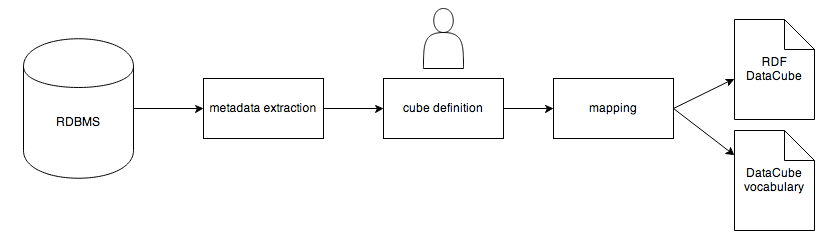
\includegraphics[width=140mm]{img/mapping-olap2dc.png}
	\caption{OLAP2DataCube mapping process}
	\label{fig:olap2dc-mapping}
\end{figure}


Let us take a brief excursion back to the OLAP2DataCube described in Section 
~\ref{rw:olap2dc}. The tool was not designed just to convert a non--RDF dataset 
into the RDF standard with respect to the DCV metaformat. Executing the tool on a 
dataset has one important side--effect: there is a new QB data structure definition
generated with bases on 
the structure of the input dataset. Therefore, the tool does not map the 
dataset to match an existing data structure definition, it creates a new one. That is definitely
needed when one transforms a non--RDF dataset into RDF. But once 
this is done, it is probable that a company or an organzation will produce the 
same kind of data periodically, therefore, they will reuse the same data structure definition.

This is the reason why we will propose a system which fill focus on the task of 
mapping the input dataset to match an existing data structure definition. 
The authors of the LDVM~\cite{ldvm} (see Section~\ref{sec:rw:ldvm}) propose to make standalone
visualizers. Each of them will 
be able to visualize a specific kind of datasets. Its visualization abilities will be described with
an \emph{input signature}. A Data Cube data structure definition could be easily transformed into
an example of such a signature. That is another reason why we want the tool to 
map the input dataset into an existing definition.

\begin{figure}
	\centering
	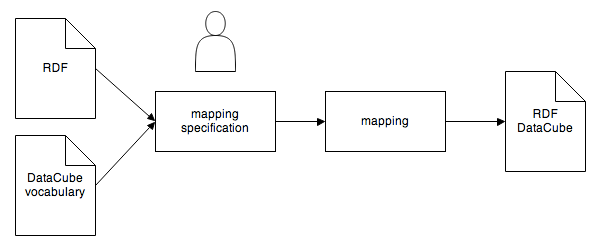
\includegraphics[width=140mm]{img/generic-mapping.png}
	\caption{RDF to DataCube mapping in a generic system}
	\label{fig:generic-mapping}
\end{figure}

That means we would like to enable the user to take an existing RDF
dataset and give it a statistical meaning. The initial thought was to
implement a set of specialized 
mapping modules. We would have to implement a standalone mapping module for
each existing Data Cube Vocabulary. Since this is rather impossible and 
surely inefficient, we made some experiments in order to ensure that we would be able to come 
up with a generic mapping component. That is why the process of the implemented
system will be similar to what is shown in Figure~\ref{fig:generic-mapping}. The 
process seen in the diagram represents a high--level view of the system. As we 
consider some additional criteria we will provide a more detailed schema of the 
proposed system. 

The biggest difference is that the original dataset can contain the statistical 
data in a not--so--obvious form, as in the case of the relational DB.
The user may need to apply an analytical 
extraction (a term introduced in~\cite{ldvm}) in order to select the transformed data.
We start with an arbitrary RDF document, 
specify the process of mapping and how the system transforms the data in order
to comply with the Data Cube Vocabulary standard. We also require the user to 
provide a Data Cube Vocabulary definition. The proposed system will map the data
to conform with such a definition.

We will now walk the reader through the decision process we have made in order to propose 
the system. As stated before, the input is an arbitrary RDF graph. To 
be able to map data from the graph to a form compliant with a Data 
Cube Vocabulary, the system also needs for a vocabulary to be a part of the input. 
As discovered in Section~\ref{datacube-vocabulary}, the vocabulary is another 
RDF graph.

Based on that fact, we concur that the system needs to contain a mechanism, which 
parses an arbitrary RDF graph and searches for DCV data structure definitions. 
We need to extract those definitions and have the user select one. The selected 
definition will be used in the upcoming steps to obtain mapping specification from 
the user. What we need to obtain is presented in 
Figure~\ref{fig:mapping-example}. On the right side the reader can see the 
generic visualization of a DCV data structure definition. A random graph is 
placed on the left side of the illustration. The dashed lines connect the resources 
from the original dataset with corresponding DCV components. Naturally, the 
figure represents an example of a mapping.

\begin{figure}
	\centering
	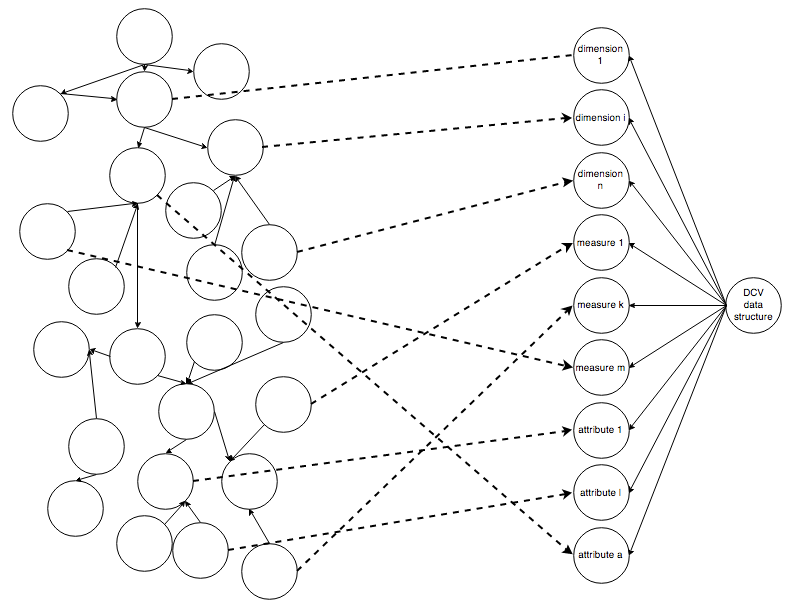
\includegraphics[width=140mm]{img/mapping-example.png}
	\caption{Mapping example. Original dataset on the left, DCV data structure definition on the right.}
	\label{fig:mapping-example}
\end{figure}

\section{Pattern selection}
We are lacking some rules telling the system how to do the mapping. 
Without such rules it is not possible to map the input graph properly. Let us 
imagine an input graph, for instance the whole DBPedia database. That represents a huge graph 
containing many facts and naturally, some of those are statistical data. But they 
are not referenced in such a context. For example the resource \emph{Prague}, which is the 
capital city of the Czech Republic has properties \texttt{populationTotal} and
\texttt{populationAsOf}. Together it creates a slice of a cube. This says that the 
city Prague (location dimension) had in a certain day (time dimension) 
a certain amount of citizens (measure).

Although this cube is originally based on a very simple pattern (a shape of a pair of cherries),
it is not possible to map such a slice into a form compliant with a 
data structure definition since the relation between the definition and the 
dataset is not defined in the original data. For a well--defined data structure 
definition and a well--defined dataset, it could be possible to propose another 
system, which would try to detect the relation and create them 
automatically. For instance, the location dimension, which is usually named
\emph{reference area} could be connected to a generic type -- a location.
Also the resource \emph{Prague} could be connected with the location type. But 
that would mean introducing a system, which would process a lot of data trying to 
match each supertype of the dimension with the properties of every resource in 
the graph. It would have to use advanced heuristics and it would probably have 
to adopt some techniques from the machine--learning field. A fully--automated 
system would also introduce a lot of mistakes into the results since it would 
be a highly experimental approach. Therefore, implementing such a system would 
not be the goal of this thesis. 

On the other hand, we would like to propose a system, which will be flexible 
enough to allow the user to take an arbitrary Data Cube Vocabulary data 
structure definition and map a reasonable part of this dataset into a compliant 
form.

Unfortunately, the phrase \emph{reasonable part} is not very scientific. 
It comes from the data semantics and it is quite difficult to formalize. What 
the user should map to a given data structure definition should have 
a corresponding semantics. For instance, if we use the population size example, the 
user should probably not map the statistics of government debts to that 
definition. Even though a country is a location, the amount of the debt represents a 
number and was certainly calculated on a specific day, therefore, the 
data match the ranges of the data structure definition components, but it does 
not match the semantics.

\begin{sloppypar}
On the other hand, we do not want to make the tool too restrictive in order to 
achieve better user experience. For instance, we have mentioned
(Figure~\ref{fig:example-dcv-dataset}) a data structure 
for the population example that declares a dimension \texttt{czso-ds-def:refArea}. 
The range of that dimension is specified as \texttt{czso-reg:Municipality}. 
With a restrictive approach, the tool would not enable the user to map the data from 
the DBPedia database to match the data structure definition, since the DBPedia 
dataset does not contain the \texttt{czso-reg} namespace. Nonetheless, Prague is 
certainly a Czech municipality. Therefore, the tool will not check the range 
while performing the mapping. If it had, the user would need to involve 
other datasets so as to provide the range--related information.
\end{sloppypar}

What is still missing is the way of informing the tool about how to map the data.
Obtaining such a specification can be implemented in many different ways. 
All of them are actually described in Chapter~\ref{chap:rw}. Some of the tools used 
their native language -- the SPARQL. That is beneficial for a developer due to 
its relatively easy implementation. But it is a bit cumbersome for a user 
who is required to know the SPARQL language. On the other hand, from all the approaches
it restricts the possibilities of the system the least. It enables the user 
to specify a wide range of mappings.

OLAP2DataCube took an advantage of the database structure (Section ~\ref{olap2dc}) --- 
especially of relational feature --- foreign keys. Since the RDF format 
is based on expressing relations it would not present an issue. But what the 
OLAP2DataCube tool did, was that it transformed already existing statistical data from
the star--shaped database structure into another format. But in the world of RDF 
data we would restrict the tool a lot if we relied only on star--shaped 
schemas, hence, we need to work with a generic graph.

Tabels introduced a custom DSL that should have made the situation easier for 
a user (Section~\ref{rw:tabels}). But as experienced while doing research for Chapter~\ref{chap:rw}, 
we did not find it very user--friendly. There certainly was a pre--generated script based
on the uploaded file but in most cases the user had to modify the script in order to
achieve desired results. The user is required to learn a 
completely new language, but will probably not find any other use of such a skill
elsewhere. Moreover, it is not an easy task to implement the 
custom DSL itself. Therefore, we consider this approach to be the worst.

The last approach we have noted is the \emph{query--by--example} introduced in 
Tabulator (Section~\ref{sec:rw:tabulator}). It was used to let the user specify what type of data patterns they are 
interested in. In the exploration mode the user was able to \emph{visually} 
specify the pattern and switch to the analytical mode. Such an approach enables 
us to construct a SPARQL query and come closer to the very first (and the least restrictive) 
approach. Nonetheless, it brings some new implementation issues.

The most obvious one is the transformation of the user's selection into a SPARQL query. 
We will also require the system to be capable of making a preview of the 
original dataset in order to offer the user a visualization. The visualization 
itself will interact with the user and provide them a way to specify the pattern.

Of course, the query--by--example does not need to be necessarily done visually. But 
obtaining an example with a non--visual approach leads to the involvement of a DSL. Even 
a simple DSL, for instance a variation of CSV format, is not as user--friendly as 
the visual approach. The visual approach also enables us to force some 
restrictions to avoid dealing with an arbitrary user input. We will 
obtain an input that is already valid.

After obtaining the pattern all the necessary information are gathered. We 
may proceed to the mapping process itself. The mapping module will query the 
data source for the data. It will use the pattern specified by the user. After 
fetching the data, it will construct a new graph containing a set of DCV 
observations. Based on what we have learnt so far, the system will appear in detail 
as shown in Figure~\ref{fig:generic-mapping-detail}.

\begin{figure}
	\centering
	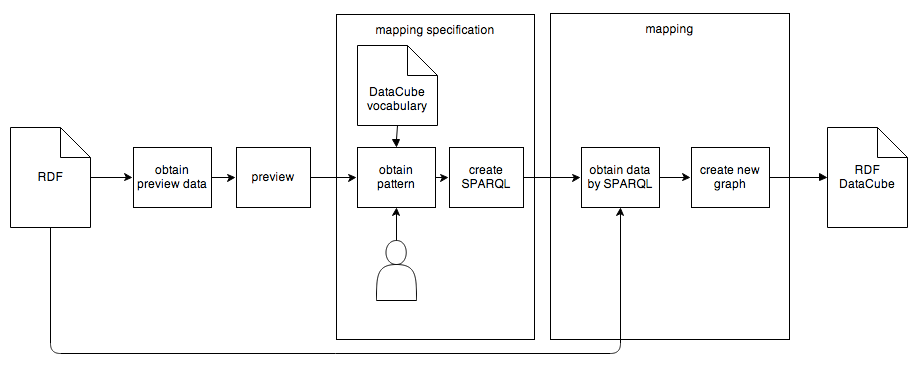
\includegraphics[width=140mm]{img/generic-mapping-detail.png}
	\caption{Detail of the proposed system.}
	\label{fig:generic-mapping-detail}
\end{figure}


\section{Mockups}
\FloatBarrier
We will show the reader our idea of a user interface of the proposed system. We 
will refine some previously outlined features, especially the pattern selection.

In the first step (Figure~\ref{fig:mockup-01}), the user is required to specify the source of the data that 
will be transformed. They will probably supply a reference to a SPARQL Endpoint,
e.g. \url{http://dbpedia.org/sparql}. The user also has to reference a graph, which contains the 
desired Data Cube Vocabulary data structure definition.
That is a URL as well, e.g. \url{http://datacube.payola.cz/dsd/population.ttl}.
The type of data source 
is needed in order to determine how to fetch the data.
\begin{figure}
	\centering
	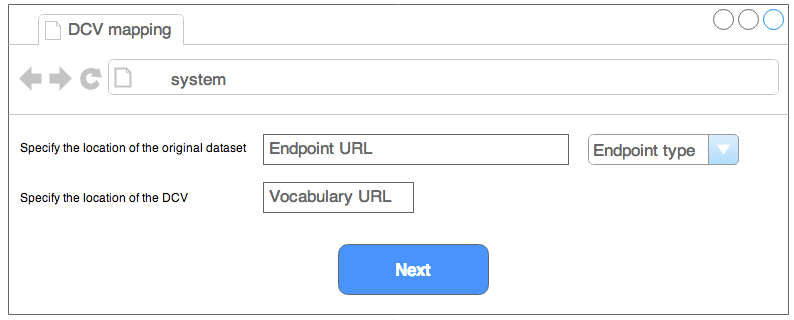
\includegraphics[width=120mm]{img/mockup-01.png}
	\caption{Step 1: data source and vocabulary specification}
	\label{fig:mockup-01}
\end{figure}

After proceeding to the next step (Figure~\ref{fig:mockup-02}),
the user will be asked to choose a DCV data 
structure definition. The definition list is prepared based on the vocabulary provided 
in the previous step. The system has already parsed the supplied graph and filtered all
DCV data structure definitions. As an example, the user will select the
\url{http://datacube.payola.cz/dsd#PopulationSizeDefinition} data structure definition.

\begin{figure}
	\centering
	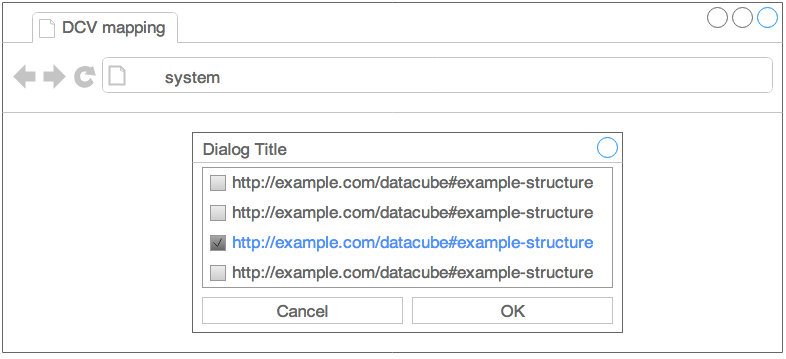
\includegraphics[width=120mm]{img/mockup-02.png}
	\caption{Step 2: DCV data structure selection}
	\label{fig:mockup-02}
\end{figure}

The system now selects data for a preview. The retrieved dataset is 
visualized and shown in a dialog (Figure~\ref{fig:mockup-03}). The user is 
required to specify a pattern. The specification is done by clicking the vertices in 
the visualized graph (some progress is shown in Figure~\ref{fig:mockup-05}).

\begin{figure}
	\centering
	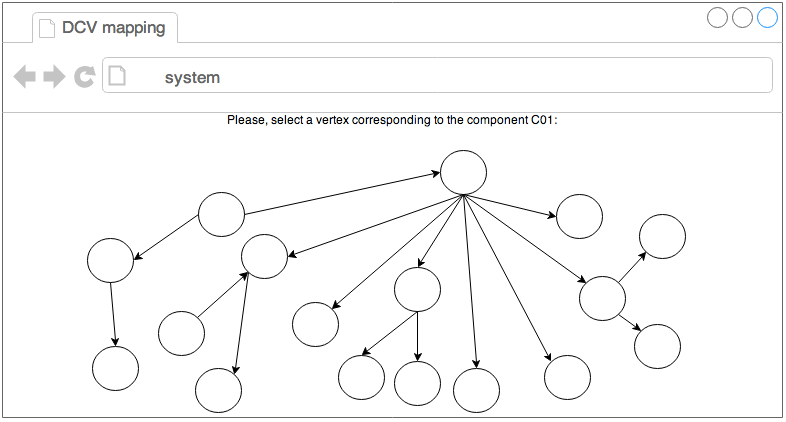
\includegraphics[width=120mm]{img/mockup-03.png}
	\caption{Step 3: Pattern selection}
	\label{fig:mockup-03}
\end{figure}
\begin{figure}
	\centering
	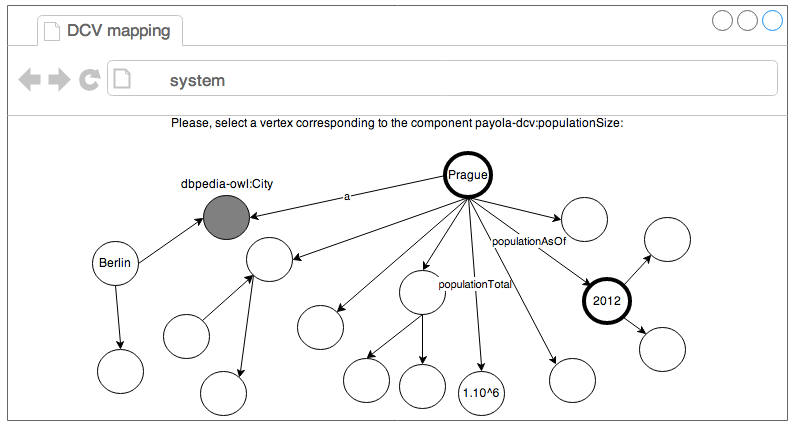
\includegraphics[width=120mm]{img/mockup-05.png}
	\caption{Step 3 (example): Pattern selection. The user has to provide an example
	for mapping the dataset to a population vocabulary. In the last step, the user is asked
	to select a vertex corresponding to the \texttt{payola-dcv:populationSize} property.
	They have already selected the vertices representing Prague and observation date
	in order to satisfy the other components. The \texttt{dbpedia-owl:City} vertex can
	be selected to refine the example, but it does not correspond with any component.
	The user is about to select the vertex connected via the \texttt{populationAsOf} 
	relation. This represents an example of selecting a meaningful pattern, which 
	is a connected graph.}
	\label{fig:mockup-05}
\end{figure}

After the pattern is specified the system has all the information it needs. The 
user is able to start the mapping process. When done, the system offers
the results (RDF graph).
\FloatBarrier

\section{Benefits of integration into Payola}
\label{why-payola}
Since we have participated on the implementation of the Payola RDF tool, we will 
now go through the pros and cons of integrating the proposed system into Payola.
We will also decide if we proceed with the integration.

In Chapter~\ref{ch:payola} we familiarized the~reader briefly with the~main
concepts of the~Payola framework. The reader also knows how the~analyses
evaluation is done. Therefore we may demonstrate the benefits arising from
the integration of the proposed system with the Payola framework.

The crucial feature of the Payola framework is the analysis subsystem. It enables a user
to combine multiple data sources and benefit from their 
combination. Based on that, a completely new set of facts can be computed.
(This could be optimized with SPARQL 1.1 and Federated queries~\cite{federated-queries}.) 
Therefore, it could be handy to introduce a Data Cube Vocabulary analytical 
plugin, which would be able to convert the results of an analysis into the Data 
Cube Vocabulary format. Such a plugin could be connected directly to an output
of a data fetcher plugin --- this will cover the basic implementation shown in 
Figure~\ref{fig:generic-mapping-detail}.

But we can go a bit further. Since it would be an analytical plugin, the user 
would be able to use such a plugin in an arbitrary step of the analysis. Let us look back again
at the DBPedia and the population statistics example. A plugin representing the proposed
system would substitute multiple different plugins 
in order to obtain the same data. In this case it is the \texttt{Typed}
plugin and the \texttt{Property selection} plugin. Those are covered based on the selected pattern.
In addition, the result would be 
compliant with the Data Cube Vocabulary standard.

Another asset is considered to be the ability to transform multiple data 
sources in one step. The users might also further use the converted datasets --- combine them
(join, union) and analyze those datasets in a unified format (specified by the DCV).

The next benefit of the integration with the Payola analyzer is that the user 
can assemble an algorithm, which is applicable multiple times. The main 
advantage is that it reflects the current state of the data sources at
the time of the execution. That means that if the data source contents get 
updated, the user just executes the analysis again and the mapping is instantly 
performed. There is no need to specify anything for the second time.
This is useful especially in a case where the analysis is more complicated than the 
mapping process itself.

As stated before, the Payola application also offers the functionality of 
sharing. This feature is usable at least in a case of sharing the results 
of an analysis. The introduction of a Data Cube Vocabulary plugin does not change anything.
The user will still be able to share the analysis. If the analysis contains just the data fetcher 
and the DCV plugins, the user shares only the mapping process.

Another aspect could be an effort needed to implement such a system. Since the 
goal of software engineering is not to implement the same systems over and over 
but to bring new systems, new features, speed up the computation process and 
bring better user experience, it makes no sense not to take advantage of 
an already existing platform. The same approach could be seen in the case of reviewed 
tools like Olap2DataCube (section~\ref{olap2dc}) or CubeViz 
(section~\ref{cubeviz}).

The Payola framework contains a variety of useful components. As an example of 
such components we might name data fetchers, RDF processing modules or 
visualization API.

Since a part of the goal of this thesis is to implement an exemplary 
visualization that takes advantage of the Data Cube Vocabulary format, it will 
be very useful to stay focused on the task and implement just the visualizer, 
instead of a lot of supporting subsystems that are already 
implemented elsewhere.

Moreover, we can take advantage of the existing visualization plugins. The basic 
one, triple table plugin, offers a quick overview of the data. The user 
will also be able to download the results of the transformation into a static 
RDF file for further use or just for simple backup purposes.

\begin{figure}
	\centering
	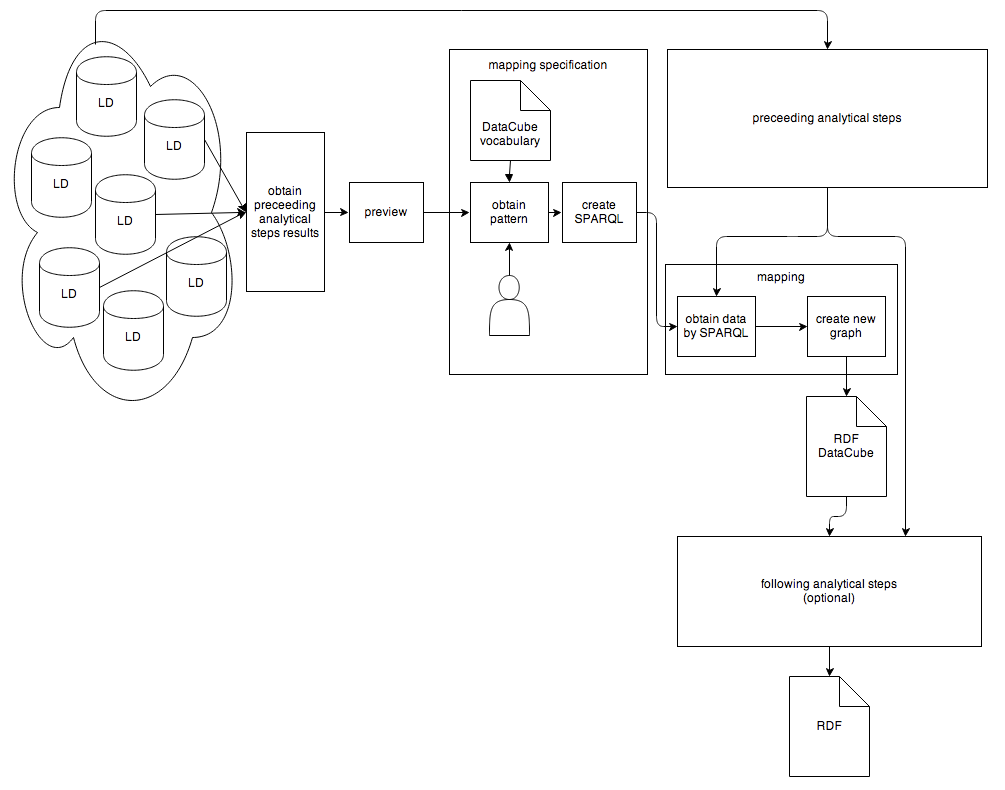
\includegraphics[width=140mm]{img/payola-mapping.png}
	\caption{Mapping process integrated into the Payola analyzer.}
	\label{fig:payola-mapping}
\end{figure}

We show a possible way of the integration of the mapping process into the Payola analytical extraction
in Figure~\ref{fig:payola-mapping}. It shows the proposed system in a context of an
analytical pipeline. Such a pipeline is constructed by the user. The process starts with querying data 
sources in order to offer the user an overview. The amount of the sources depends 
on which sources are involved in the analytical pipeline. They are fully independent 
and spread throughout the whole Internet. The obtained data are visualized to 
the user who is required to select a pattern. Since we need to guide the user 
to select a proper one, we also need them to specify a Data Cube Vocabulary. 
We will need to parse the Vocabulary, extract the DCV datastructure definitions 
and offer the user a list of the available definitions. After they choose one, we will be able to determine how many mapping references we need the 
pattern to contain. The number is, of course, based on the amount of components 
within the datastructure definition. We will construct a SPARQL query based on the selected pattern.

The rest of the process is a common analytical pipeline execution. The Data Cube 
Vocabulary plugin can be interpreted as a standard plugin. Since the 
transformation is done by executing a SPARQL query, it corresponds with an 
execution of a SPARQL query plugin. During the evaluation of the analytical pipeline we reach a certain point of an undergoing mapping (thanks to a DCV plugin). On the output of this plugin, we will for certain find a dataset compliant with the DCV standard. But the dataset need not 
be the result of the analytical pipeline execution. It may be used as an input 
for the upcoming analytical steps.

Based on facts presented in the text above we find it reasonable to integrate 
the proposed system into Payola.

\section{Formalization}

In this section, we are going to formalize the aforementioned process a bit 
more. We need to specify the input of the system. We will also 
provide a definition of the mapping process. A description of the output will be 
also presented.

\subsection{Input and output}

The input of the system will be an arbitrary RDF graph $G_{input}$ as shown
in Figure~\ref{fig:mapping-example}. It will be mapped into a form compliant
with the DCV standard. Since the DCV also takes advantage of the RDF standard,
the result will likewise be a graph, let us say $G_{output}$.

\begin{figure}
	\centering
	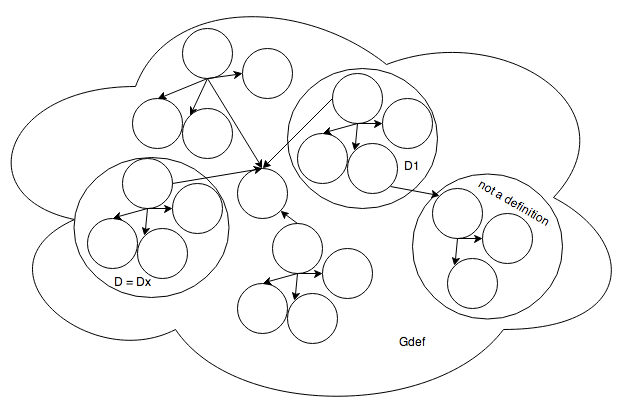
\includegraphics[width=120mm]{img/definition-in-graph.png}
	\caption{A user will provide an arbitrary RDF graph $G_{def}$, which may contain more than one definition. The user will select only one to work with, $D$.}
	\label{fig:definition-in-graph}
\end{figure}

As stated before, the system will have another input --- a data structure 
definition. The Data Cube Vocabulary standards are built on top of the RDF as described in the 
section~\ref{datacube-vocabulary}. That means, that a data structure is also a 
graph. We will denote the user--provided definition as $D$. But the user will probably not 
supply just a definition. They will provide an arbitrary graph, which contains the definition $D$ 
(or even more definitions) as a subgraph (see Figure~\ref{fig:definition-in-graph}).
We will denote a graph
supplied by the user as $G_{def}$. The system has to extract a list of all the definitions
(let us say $D_1, ..., D_d$) from the graph $G_{def}$. As shown in Figure~\ref{fig:mockup-02},
the user will select one of the offered definitions, for instance $D = D_x (1 \leq x \leq d)$.
The graph may contain also other data, not only DCV definitions. It is true 
that:\\

{\centering $D \subseteq G_{def}$ \\[0.5cm]}

But having the graphs $G_{input}$ and $D$ 
is not enough. We require the user to specify also an example pattern (based on the
query--by--example principle). Since all the inputs and outputs are RDF
graphs ($G_{input}$, $G_{def}$, $D$, $G_{output}$), we can take 
advantage of some existing approaches specialized on RDF transformation. 
A technically simple but powerful way, is to utilize the SPARQL language. Based on what we have introduced before, we are able to transform a user--selected pattern into a form of a SPARQL
query. We will talk about such a query as of a \emph{transformation query} and denote it $Q_t$.

What we have now is an information about what is needed on the input and 
what the result would be:

{\centering $(G_{input}, G_{def}, Q_t) \rightarrow G_{output}$ \\[0.5cm]}

In fact, the user will make the selection of the definition $D$ before the 
mapping starts. Therefore, we can extract the definition $D$ from the 
generic graph $G_{def}$ and use it as a part of the input. That is possible because 
the system does not require an arbitrary RDF graph $G_{def}$. It requires the DCV 
data structure definition $D$. The rest is done in order to improve the user 
experience. Therefore:\\

{\centering $(G_{input}, G_{def}, Q_t) \rightarrow (G_{input}, D, Q_t) \rightarrow G_{output}$  \\[0.5cm]}

What we still do not have is a description of the SPARQL query used to transform the 
data in order to obtain the output graph $G_{output}$. The form of the query is dependent on the 
definition $D$. To be more accurate, the definition $D$ contains
a set of components ($C_1, ... , C_n$), which represents dimensions, measures and attributes. Let us say, that the 
structure has defined $n$ components, $m$ measures, $d$ dimensions and $a$ 
attributes. It is true that\\

{\centering $n = m+d+a$ \\[0.5cm]}

For each n--tuple matched in $G_{input}$, the output graph $G_{output}$ will contain a node with $n+2$ 
neighbours (+1 for \verb|qb:Observation| and +1 for \verb|qb:dataSet| --- first two statements
in Figure~\ref{fig:output-graph}). A concrete example of an observation is shown 
in Figure~\ref{fig:output-graph-instance}.

The result will comply with the template shown
in Figure~\ref{fig:output-graph}. $O_i$ denotes an identifier (URI) of the generated 
observation, $S$ stands for an identifier of the input dataset,
$T_{Dim_1}$~...~$T_{Dim_d}$ stands for the type of a corresponding dimensions 
from the given data structure definition, similarly for
$T_{Msr_1}$~...~$T_{Msr_m}$ -- measures and
$T_{Attr_1}$~...~$T_{Attr_a}$ -- attributes. $R_{i,1}$~...~$R_{i,n}$ stands for
resources matched in the input graph $G_{input}$, moreover, it means that the value 
of the dimension $T_{Dim_1}$ is $R_{i,1}$, etc.

\begin{figure}
  \centering
  \begin{tabular}{lll}
$O_i$~~~~~~~~~~~~& a~~~~~~~~~~~~~~~~~~~~~~~~~& qb:Observation ;\\
          & qb:dataSet    & $S$ ;\\
          & $T_{Dim_1}$ & $R_{i,1}$ ; \\
          & $...$              & $...$ \\
          & $T_{Dim_d}$  & $R_{i,k}$ ; \\
          & $T_{Msr_1}$  & $R_{i,l}$ ; \\
          & $...$              & $...$ \\
          & $T_{Msr_m}$ & $R_{i,m}$ ; \\
          & $T_{Attr_1}$  & $R_{i,o}$ ; \\
          & $...$              & $...$ \\
          & $T_{Attr_a}$  & $R_{i,n}$ . \\
\end{tabular}
\caption{Description of an output graph node (turtle notation)}
\label{fig:output-graph}
\end{figure}

\begin{figure}
  \centering
  \scriptsize
  \begin{tabular}{lll}
\textless http://ex.com/observed\#1234\textgreater & a& qb:Observation~;\\
          & qb:dataSet    &  \textless http://dbpedia.org/sparql\textgreater ~;\\
          & my-population:count & '10233222' ; \\
          & my-population:location & \textless http://dbpedia.org/page/Prague\textgreater ~;\\
          & my-population:time  & '2012-02-23' . \\
  \end{tabular}
\caption{A concrete instance of the pattern shown in Figure~\ref{fig:output-graph}}
\label{fig:output-graph-instance}
\end{figure}

\subsection{Transformation query}

The last unanswered question is how the query $Q_t$ should look like. 
It would certainly not be an arbitrary query. Let us analyze the situation and 
walk the reader through the process of coming up with a set of constraints for the 
query.

It should be obvious that the query $Q_t$ will generate a new graph
(in fact, it will generate the graph $G_{output}$) based on some specific rules
(see Figure~\ref{fig:mapping-example}). 
Therefore, it would be a CONSTRUCT query. It is also very clear what kind of 
triples it will generate; the pattern is shown in Figure~\ref{fig:output-graph}.
The only thing we need to sort out is retrieving the resources $R_{i,1}, ... R_{i,n}$.

\subsubsection{Pattern}
\label{sec:pattern-definition}
The process of resolving those resources depends on the input graph $G_{input}$.
We will demonstrate it on the most simple case --- a 2--dimensional data structure 
definition. Such a definition requires us to specify how to select a 3--tuple of resources from 
the graph (2 dimensions, 1 measure).
We will present some ideas while using the example of the population size.

The initial idea could be that we need a country, therefore, we map all the 
countries to the \texttt{refArea} dimension, all instances of time to the \texttt{refPeriod} 
dimension and all instances of \emph{numbers} to the measure. But that is not sufficient. At first,
we need to make sure that all instances of numbers 
really express an amount of citizens in a country. Moreover, we need to map the
matching amount of citizen to a corresponding country. Therefore, all the 
selected resources need to be connected with the rest. We need to select a 
specific pattern, which will contain the relation between the resources.

\begin{figure}
	\centering
	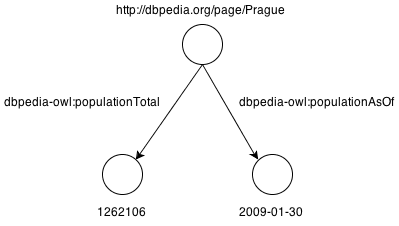
\includegraphics[width=80mm]{images/cherry.png}
	\caption{Cherry--shaped pattern example.}
	\label{fig:cherry}
\end{figure}

\begin{figure}
	\centering
	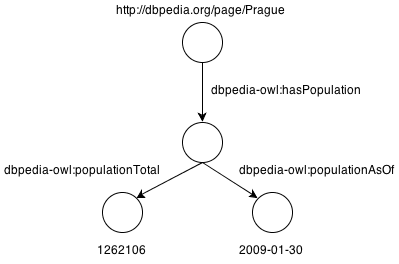
\includegraphics[width=80mm]{images/cherry_blank.png}
	\caption{The example from Figure~\ref{fig:cherry} extended with a blank node.}
	\label{fig:cherry-blank}
\end{figure}

We will use an example from DBPedia, 
the Czech Republic resource. The resource itself reference to a location, 
therefore, it should be mapped to the \verb|refArea| dimension. It has got a 
\verb|populationTotal| property, which should be mapped to the measure. Last, but not 
least, it has the \verb|populationAsOf| property, which should be mapped to the 
\verb|refPeriod| dimension.

That gives us a simple shape of a cherry--pair as shown in
Figure~\ref{fig:cherry}. But what 
if the resource us connected to a blank node with an edge of type 
population and the blank node has two properties --- size and time
(see Figure~\ref{fig:cherry-blank})?
It is clear now that there could be in the least a long oriented path between the participating 
vertices.

While keeping this fact in mind, we can accede to assembling a formula of a generic pattern used for an extraction of the resources from the original graph $G_{input}$. But 
there is one piece of a puzzle still missing. While analyzing all the
possibilities, until now we assumed that the pattern \emph{starts} (in the topological order)
with a resource, which represents one of the data structure components. But that is not  
the case.

The most simple example is the observation pattern itself. The 
entities come together but their connection is dependent on a completely 
different resource. We reference such an entity
as a \emph{reference vertex}. Any pattern vertices corresponding to a component from the 
data structure definition could also match the \emph{reference vertex}.

Later on, we have discovered that such a kind of patterns is not what the user 
wants to select. We have applied too much restrictions. Such a pattern
represents only a subset of patterns the user may want to select. We have learnt
that the most concrete designation of such a pattern is the well--known term:
\emph{connected graph}.

We left out the term \emph{oriented} on purpose. While experimenting with the 
system, we had discovered that for purposes of the pattern specification the 
orientation is not necessary. We need all the referenced vertices to have a 
relation between each other, but the orientation does not matter.

In order to get the reader familiar with some 
approaches we will utilize while implementing the system, we are about to point 
out some facts.

We are about to build a pattern $P$. The pattern reflects an example set by the user,
an example that represents the user’s proceedings of the data mapping to the components from a data structure definition. The pattern will
be used later to construct the desired
transformation query $Q_t$. As shown in Figure~\ref{fig:mapping-example}, we 
require the user to find an equivalent for each component ($\{C_1, ... C_n\}$) of the data
structure definition $D$ in the input graph $G_{input}$. The equivalent for $C_1$ is in 
Figure~\ref{fig:output-graph} denoted as $R_{i,1}$. But there are many other 
equivalents for the component in the input graph ($R_{i,1}$ is one of many instances). 
That is why we need to generalize the symbols used for matching 
resources. Therefore, we introduce a new set of symbols, $M_1, ..., M_n$ to 
express that such a resource is a vertex matched in the mapping process, $M_1$ 
for component $C_1$, etc. To understand this better, see Figure~\ref{fig:mapping-pattern}}.

\begin{figure}
	\centering
	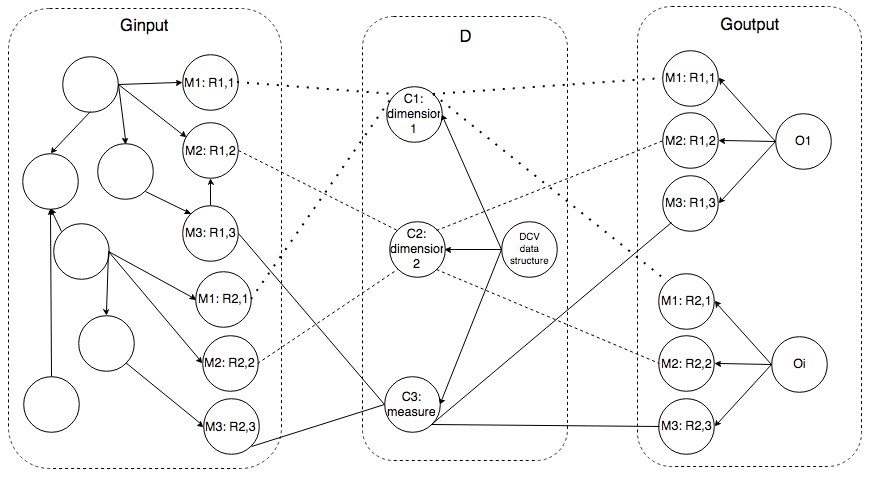
\includegraphics[width=140mm]{img/mapping-pattern.png}
	\caption{An example of mapping. $G_{input}$ is an input graph, $D$ a data 
	structure definition, $G_{output}$ an output graph. Lines between those graphs represent mapping.
	For each component $C_1, ..., C_n$ we need the user to give an example of a matching entity.
	That means one concrete instance $R_{i,1}$ for component $C_1$. Such match is generally denoted
	as $M_1$.}
	\label{fig:mapping-pattern}
\end{figure}

Please, keep in mind that we are about to construct a 
connected graph. Therefore, we define an invariant, which says that in every 
step of the pattern construction the pattern $P$ needs to be a connected graph.

As shown in Figure~\ref{fig:mockup-03} and Figure~\ref{fig:mockup-05},
the system iterates over data 
structure definition components and lets the user select an example of a 
vertex corresponding to the current component.

For each component we are about 
to extend the constructed pattern. We will take advantage of the notation from the
graph theory, because the pattern is also a graph (let us remember the connected graph invariant).
Therefore, in the beginning:\\

{\centering $P = (V = \emptyset, E = \emptyset)$ \\[0.5cm]}

We will extend the pattern $P$ for each component $C_1, ..., C_n$ of the 
definition $D$. We need the pattern to contain all the vertices from $\{M_1 ,..., 
M_n\}$, because they represent examples of each component. An example of
a pattern extension for a component is shown in 
Figure~\ref{fig:pattern-enhancement}.

In order to maintain the invariant, we will enable the user to add only such 
vertices that are somehow related with an arbitrary vertex already contained in 
the pattern $P$ (an element of set of vertices $V$ --- vertices $a,b,c,d$
in Figure~\ref{fig:pattern-enhancement}, step 1).
To make it more formal, let us remind the reader that an edge is a tuple 
of vertices (e.g. $(v_1,v_2)$). In case of an oriented graph, it depends on the order within 
the tuple.

Therefore when adding an arbitrary vertex $v_i$, we demand that there exists an 
edge $e$ for which it is true that:

\begin{center}
{$e = (v_i,v_x)$ or $e = (v_x, v_i)$ \land $v_x \in V$ \\[0.5cm]}
\end{center}

\begin{figure}
	\centering
	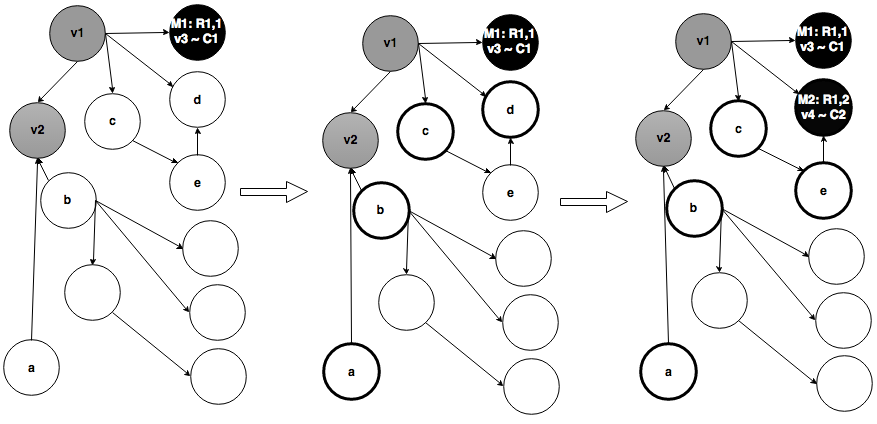
\includegraphics[width=140mm]{img/pattern-enhancement.png}
	\caption{An example of pattern extension. We start with three selected vertices
	-- $v_1, v_2, v_3$. Due to the invariant, we are able to extend the pattern only with
	the vertices $a,b,c,d$. We choose the vertex $d$.}
	\label{fig:pattern-enhancement}
\end{figure}

Of course, this is not possible to apply in the first step since the graph $P$ is empty. 
In order to make the pattern more accurate or more restrictive to obtain a more 
efficient transformation query, the user may want to reference some other 
vertices and not only the component equivalents.
Because of that observation, for each component from $C_i \in \{C_1 ,..., C_n\}$ the pattern is 
extended by adding a set of vertices $V_i = \{v_{i_1}, ..., v_{i_u}\}$ and set of corresponding edges 
$E_i$:\\

{\centering \forall $C_i \in \{C_1 ,..., C_n\}$: $P = (V = V \cup V_i, E = E \cup E_i)$ \\[0.5cm]}

In Figure~\ref{fig:pattern-enhancement} we make two steps. In the first one, we 
can add vertices $a,b,c,d$ and we choose to add $d$. That means that we extend 
the set of vertices $V$ with the set $V_i = \{v_4 = d\}$ and the set of edges $E$ with 
the set $E_i = \{(v_1,v_4 = d)\}$.

Because of the invariant:\\

{\centering $\exists e \in E_i: e = (v_{in}, v_{out}) \land (v_{in} \in V \lor v_{out} \in V)$\\[0.5cm]}

and of course:\\

{\centering $M_i \in V_i \subseteq V$ \\[0.5cm]}

--- the example equivalent $M_i$ for component $C_i$ was also selected. One of the 
added vertices from $V_i = \{v_{i_1}, ..., v_{i_u}\}$ is equal to $M_i$ ($v_3$ is equal to $M_1$
in Figure~\ref{fig:pattern-enhancement}).
   
By applying the described approach, we get a connected graph, where:\\

{\centering $\{M_1, ..., M_n\} \subset V$ .\\[0.5cm]}

That means, that the pattern covers our needs. Now, we are about to present
a generic form of the pattern, which will come out from 
such an approach. The pattern is shown in Figure~\ref{fig:sparql-pattern}. 
$n$ of the vertices from the $\{v_1, ..., v_v\}$ matches vertices $M_1, ..., M_n$.

\begin{figure}
\begin{Verbatim}[commandchars=\\\{\},codes={\catcode`$=3\catcode`_=8}]
  CONSTRUCT \{
    []   a   <http://purl.org/linked-data/cube#Observation> ;
         <http://purl.org/linked-data/cube#dataSet>   $S$ ;
         $C_1$      $M_1$ ;
         ...   
         $C_i$      $M_i$ ;
         ...   
         $C_n$      $M_n$ .
  \} WHERE \{
    \{
      SELECT DISTINCT ?$M_1$ ... ?$M_n$
      \{
         $v_1$     $E_1$     $v_2$
         $v_2$     $E_2$     $v_3$
         ...
         $v_{i-1}$   $E_{i-1}$    $v_i$
         $v_i$     $E_i$      $v_{i+1}$
         ...
         $v_{v-1}$   $E_{v-1}$    $v_v$
      \}
    \}
  \}
\end{Verbatim}
\caption{Pattern of the transformation SPARQL query}
\label{fig:sparql-pattern}
\end{figure}

\section{Visualizers}
In the beginning, we promised to implement an exemplary visualization.
Unfortunately, the Data Cube Vocabulary standard covers a wide variety of data domains, 
therefore it is hard to make a decision and choose, which visualization should be offered.

Based on what we have seen while exploring tools described in 
Chapter~\ref{chap:rw} and keeping in mind the rules of a so--called 
\emph{visualisation mantra} (Section~\ref{sec:rw:mantra}}), we decided to implement two visualizers, 
TimeHeatmap and Universal DCV. 

\subsection{TimeHeatmap}
The decision to implement this visualizer was based on the example of the population size data
presented in Chapter~\ref{ch:statistical-data}. A table or a bar chart is 
definitely a reliable way of presenting this kind of data. But while getting 
familiar with Data Cube Vocabulary, we found out that it is very popular to 
visualize geospatial data. A visualization on a map is easy to understand and is
very popular among the non--technical people. It helps to popularize Data Cube 
Vocabulary. This is also the correct type of visualization for data journalists we 
have mentioned before.

As the name suggests, this visualizer is able to handle datasets with two 
kinds of dimensions. The first one will express the time of the measurement, the 
second one will cover its location. It will support one measure that has to be 
a number.

We will place a heatmap layer over a standard map layer. The layer will express 
the intensity of the measured value in respect to the others. The scale will go from 
green to red where the latter represents the largest value measured.

\subsection{Universal DCV}
Implementing a domain--complete library of visualizers is a long--term project. 
Despite the fact, we would like to offer a visualizer, which would enable the 
user to visualize a large amount of datasets in a comfortable way. While
experimenting we have experienced on our own some discomfort in reading triple tables.

That is why we have decided to implement a visualizer, which takes advantage of 
the idea behind faceted browsers. We presented some of those in 
Chapter~\ref{chap:rw}. Therefore we would like to implement a visualizer that will 
enable the user to slice visualized datasets and prepare usual visualizations of 
the slices. A mockup of such a visualizer is shown in 
Figure~\ref{fig:dcv-universal}. It should contain a pie chart and a bar chart 
visualization.

\begin{figure}
	\centering
	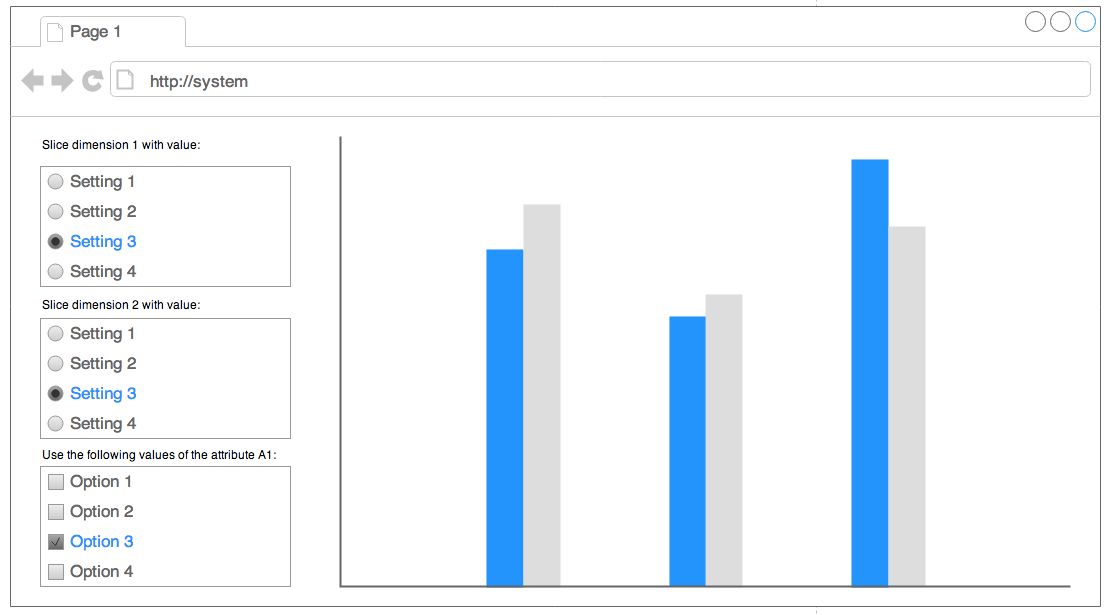
\includegraphics[width=140mm]{img/dcv-universal.png}
	\caption{Data Cube Vocabulary universal visualizer.}
	\label{fig:dcv-universal}
\end{figure}




\chapter{Implementation}
\label{ch:implementation}
In this chapter we~would like to~walk the~reader through the~process of~implementing 
the proposed system. Naturally, one of~the~possibilities was to~implement a~completely new system, 
which would comply with our requirements. But since we~participate on~a development of~a~large RDF
application -- Payola; and based on~the facts from
Section~\ref{why-payola}, we~had decided to~implement the~proposed system as~a~plugin
for Payola. This will affect the~implementation by~fetching into~specifications a~few non--functional
requirements.

Before we~start, let us~mention again some tools whose authors decided to~do the~same --- to~integrate them into~a~larger project. We~are talking specifically about 
OLAP2DataCube(Section~\ref{olap2dc}) and CubeViz (Section~\ref{cubeviz}),
which are based on~the~OntoWiki platform developed by~the AKSW~\cite{aksw} group at~the~University of~Leipzig~\cite{leipzich-uni}.

We would now like to~describe in~detail the~process of~integration of~our proposed system with
Payola. However at~first, we~need to~provide a~description of~Payola internals, thus presenting all
the facts that we~deem necessary, in~order to~make the~implementation fully understandable to
the reader.

\section{Integration of~the proposed system}
We will build up~on the~brief description from Chapter~\ref{ch:payola} and familiarize the~reader
more with the~architecture of~Payola. We~will especially
focus on~those parts that were important to~the integration of~the proposed system.

Payola is~a web application. It~is built on~top of~a Scala MVC framework (Play! 2.1~\cite{playfw}).
Payola takes advantage of
some modern web technologies like HTML5 (especially the~canvas element).
Therefore, we~will implement the~system as~a component of~a web application.
We could have implemented the~tool as~a standalone 
application (e.g. a~console or~web a~service) with a~certain kind of~API,
but that would have meant less than full advantage of~some of~the Payola framework features.
It would not allow us~to profit from all the~benefits described in~Section~\ref{why-payola}. 

\emph{We are used to~talk about Payola as~either an~application or~a tool or~a framework. To
distinguish those terms we~consider Payola to~be an~application (or a~tool) from the~user’s
point of~view whereas we~are looking at~it as~a framework from the~developer’s side.}

As described in~Section~\ref{why-payola}, the~most beneficial way of~implementing the~proposed system into~Payola is~as an~analytical plugin. In~Chapter~\ref{ch:payola}
we have got the~reader acquinted with the~general principles of~how the~analyses and plugins work. We~have also provided some examples 
of already existing plugins. We~are about to~widen the~variety of~plugins and 
introduce a~new one.

\section{Analytical plugins}
Before moving forward, one needs to~understand the~technical 
details behind the~analytical plugins. We~have already stated that such a~plugin is~a computation unit. Its task is~to transform the~input graph(s) into~one output 
graph. The~transformation fully depends on~the implementation of~such a~plugin. Each plugin has always exactly one output but may have infinite number of~inputs. It~might also have no~input at~all. For instance, all the~data 
source plugins that fetch data from some kind of~storage, are generally considered to~be
graph generators. That is~why they have no~inputs. The~Filter 
plugin filters the~input graph by~applying a~specified constraint. That is~why it~has one input (the constraint is~applied on~a single graph).
An example of~a plugin with more than one input is~known as~the~\textt{Union} 
plugin, which takes two graphs and combines them together.

One can see that this is~perfectly suitable for completing our task --- we~are about to~implement a~system that will transform an~input graph into~a~different one.

In the~case of~the~texttt{Filter} plugin, we~spoke about \emph{specifying a~constraint}. The~plugin has parameters that enable its reuse in~multiple--case scenarios. For instance,
the Data Fetcher plugin has a~parameter, which tells 
the plugin where to~fetch the~data from. It~would be~to no~avail had we~implemented a~plugin
enabling the~user to~fetch the~data solely from DBPedia (the fact that it~is one of~the largest data
sources notwithstanding).
The original implementation of~Payola recognized 4 different types of~plugin 
parameters --- \texttt{string}, \texttt{float}, \texttt{int} and \texttt{boolean}. 

If the~reader were to~remember Chapter~\ref{ch:proposal}, they would recall that we~determined that 
the system would need the~following input:
\begin{itemize}
  \item An~arbitrary RDF graph.
  \item A~graph containing the~DCV data structure definition.
  \item A~transformation pattern.
\end{itemize}

At this point we~should decide, which of~them would become parameters and which of~them inputs of~the plugin. It~may seem to~be a~good idea to~supply the~graphs as~inputs and the~transformation pattern as~a parameter. At~least, it~is 
consistent with the~idea that a~graph is~an input type of~an analytical plugin. 
But if~we think about it~just a~bit longer we~realize that once we~have the~transformation SPARQL query, we~do not need the~data structure definition for 
processing anymore. We~just need the~plugin to~receive the~input data and transform 
them while applying the~transformation query.

We need from the~data structure definition to~only inform the~user as~to what kind of~data are they 
are working 
with. We~require them to~select a~valid and meaningful pattern. 
Therefore, we~need for the~plugin to~have one input (the arbitrary RDF dataset) and 
one parameter (the transformation pattern). Under normal circumstances
that would be~sufficient, but we~need to~find a~way of~storing the~data structure definition metadata in~order 
to present them to~the user if~necessary.

When we~started experimenting with the~system, the~idea of~specifying the~transformation pattern was a~little bit different. Initially, we~thought that it~would be~possible to~specify a~pattern for each DCV component separately. After 
a while, we~had learnt that it~makes the~task harder for the~user. It~is more complicated to~select a~valid pattern, especially when the~pattern needs to~be a~connected graph for a~conclusive expression
of the~relations between matched entities.

In the~process of~experimenting, we~came up~with a~new way of~storing the~data structure definition within an~analytical plugin. We~made each component to~be a~parameter in~order to~enable the~user to~select a~pattern for each of~them. Such an~approach was an~unexplored territory in~the scope of~the Payola framework.

\begin{figure}
	\centering
	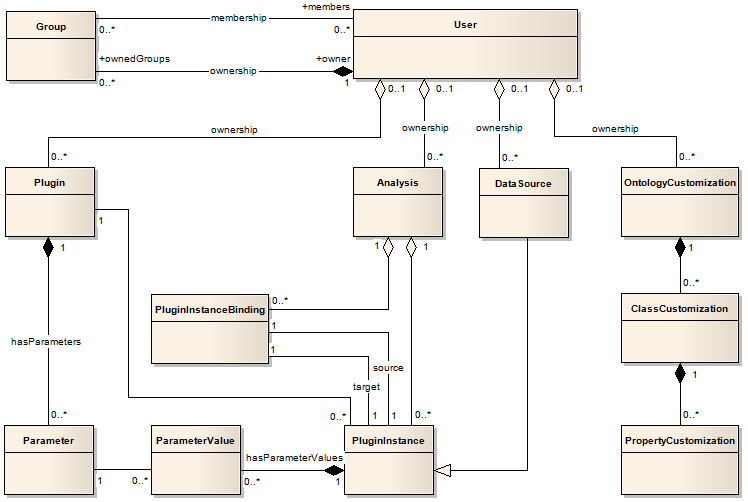
\includegraphics[width=140mm]{img/params-schema.png}
	\caption{Payola entities schema containing a~schema of~the parameters 
	subsystem of~the Payola framework.~\cite{payola:dg}}
	\label{fig:params-schema}
\end{figure}

The architecture of~the parameters subsystem can be~deduced
from a~schema in~Figure~\ref{fig:params-schema}. We~distinguish between two 
different basic types of~entities -- \texttt{Plugin} and \texttt{PluginInstance}. The~first 
one represents a~template for each plugin type. An~instance of~the second one is~created for
each occurrence of~the plugin in~an analytical pipeline. Whilst an~instance of~the \texttt{Plugin}
class defines the~number of~parameters, an~instance of~the \texttt{PluginInstance} 
defines their values.

For instance, the~Filter plugin implementation is~coded in~the class \texttt{Filter}.
That class is~derived from the~\texttt{Plugin} abstract class. There is~a single record in~the database table
\texttt{plugins}, which represents the~information about the~Filter plugin existence.
Among others, it~contains the~FQDN of~the \texttt{Filter} class. This course will inform the~analytical
pipeline evaluator which class is~responsible for handling
a specific type of~plugin. The~class also defines that the~Filter plugin has 3 parameters. It~even 
defines their data types. One single instance of~such a~class is~sufficient. On~the other hand, we~need
multiple instances of~the \texttt{PluginInstance} class in~order to
handle parameters values. Each occurrence of~the Filter plugin will be~probably 
used with a~completely different set of~parameters (while having the~same count).

\begin{figure}
	\centering
	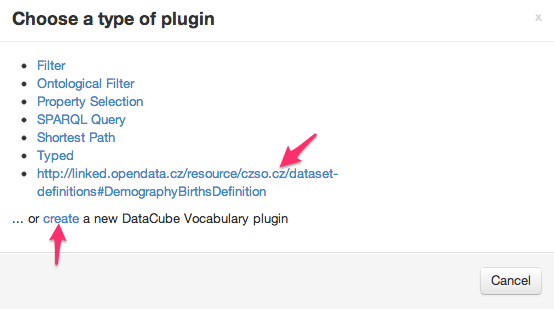
\includegraphics[width=100mm]{img/choose-plugin.png}
	\caption{A user is~able to~create a~new DCV plugin or~to connect an~existing one.}
	\label{fig:choose-plugin}
\end{figure}

The aforementioned features enabled us~to implement what is~shown in~Figure~\ref{fig:choose-plugin}. When adding a~new connection into~the~analytical 
pipeline the~user is~able to~create a~new DCV plugin or~connect an~existing one. 
To create a~new one, the~user is~required to~supply an~URL of~a graph containing 
a chosen vocabulary (see Figure~\ref{fig:create-plugin}). After processing the~supplied graph, the~user is~required to~choose a~desired definition as~shown in~Figure~\ref{fig:choose-def}.

\begin{figure}
	\centering
	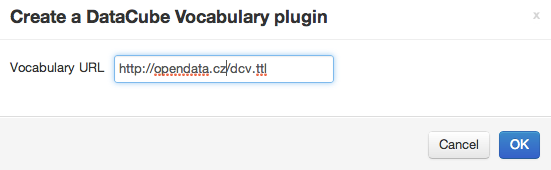
\includegraphics[width=100mm]{img/create-dcv.png}
	\caption{To create a~new one, the~user is~required to~supply an~URL of~a graph containing 
a chosen vocabulary.}
	\label{fig:create-plugin}
\end{figure}


\begin{figure}
	\centering
	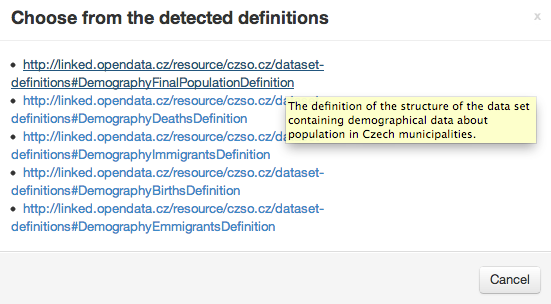
\includegraphics[width=100mm]{img/choose-def.png}
	\caption{A list of~detected DCV definitions is~shown to~the user.}
	\label{fig:choose-def}
\end{figure}

\subsection{Data Cube Vocabulary analytical plugin}

\begin{figure}
  \begin{verbatim}
/**
  * @param _name Name of~the plugin.
  * @param _inputCount Count of~the plugin inputs.
  * @param _parameters The~plugin parameters.
  * @param id~ID of~the plugin.
  */
abstract class Plugin(
    protected var _name: String,
    protected val _inputCount: Int,
>    protected val _parameters: immutable.Seq[Plugin#ParameterType],
    override val id: String = IDGenerator.newId) ...
  \end{verbatim}
  \caption{The header of~the \texttt{cz.payola.domain.entities.Plugin} class. It~does not restrict the~count
  of~the passed parameters, it~receives a~generic sequence.}
  \label{fig:plugin-trait-code}
\end{figure}

In the~case of~the implemented plugin, we~take advantage of~the fact that the~\texttt{Plugin} abstract class allows us~to pass a~variable count of~parameters to~the 
plugin implementation. See Figure~\ref{fig:plugin-trait-code} to~learn how the~abstract class header 
looks like. That is~beneficial mostly due to~every vocabulary being consisted of~a 
different count of~components. But we~need to~create an~instance of~the \texttt{Plugin} entity
for each vocabulary in~order to~store the~components metadata.

Until now, there was usually just one entity derived from the~type \texttt{Plugin} associated with
a codebase of~a plugin. The~concept of~plugins was not formerly designed to~have
a variable count of~parameters for each plugin instance.

That is~why we~have decided to~acquire a~new approach. By~adding a~plugin 
into the~analytical pipeline we~will give the~user an~opportunity to~create a~new instance of~the \texttt{Plugin} class. This instance is~based on~a specified data structure definition
with an~appropriate count of~parameters. Each parameter represents a~component 
of the~data structure definition. Moreover, a~\texttt{Plugin instance} is~instantly created 
based on~the formed \texttt{Plugin} template. A~representation of~that instance is~consequently 
rendered into~the~pipeline editor and the~instance itself bound into~the~analytical pipeline.

\begin{sloppypar}
Let us~present a~short example and consider an~exemplary data structure definition \texttt{example:population}
consisted of~3 
components; let us~say dimensions \texttt{example:refArea}, \texttt{example:populationAsOf}
and measure \texttt{example:populationCount}. Such a~data structure leads us~to 
the creation of~a new plugin of~type Data Cube Vocabulary named 
\texttt{example:population}. It~would have 3 parameters named in~the same way the~components are, all of~type \texttt{string}.
\end{sloppypar}

Such an~implementation fits into~the~Payola architecture. Moreover, as~a side--effect, it~brings
an added value --- based on~the data structure definition, a~plugin is~created. 
That means that there will be~a specific plugin for each DCV data structure 
definition. That plugin can be~owned by~the user who initiated its creation. 
From that point onward, the~plugin will be~available to~the user and they
will not need the~data structure definition anymore. What we~got is~a 
component, which is~reusable on~the level of~an analyzer. Since the~user is~able to~share their custom plugins with other Payola users, they are
naturally able to~share the~created Data Cube Vocabulary plugin, too. 

An important fact is~that regardless of~the amount of~the parameters, it~is sufficient 
to have a~single codebase. We~will implement a~single Scala class that represents the~behaviour 
of the~plugin. That is~because the~\texttt{Plugin} abstract class (Figure~\ref{fig:plugin-trait-code})
from the~Payola framework
API does not constrain the~count of~parameters supplied to~the class.

This however causes a~different kind of~a problem. As~we have stated before, the~approach to~selecting a~pattern per each component does not align well with what we~need. Only a~few lines above we~also discovered that all that is~needed is~a 
single parameter --- a~transformation pattern. Therefore, we~need to~modify a~bit the~behaviour of~the analytical pipeline editor in~order to~render the~\texttt{Plugin instance}
in a~non--generic way. We~will also coerce the~plugin to~always store the~transformation query 
within the~first parameter.

We realize that this approach is~not quite clean nor nice but we~need to~accept it~for several reasons.
The first being a~simultaneous research based on~the original Payola done by~various people where
at the~time of~writing this thesis and experimenting with the~proposed system, some of~the researchers 
would not be~able to~overcome the~major architectural change and thus not finish their project.
But such a~change would have been required since 
it would have been necessary to~introduce a~new parameter into~the~\texttt{Plugin} trait. 
It would demand something general enough to~carry metadata that are not determined for 
computational purposes (and distributed together with the~plugin throughout the~whole system).
It would have also been extremely difficult to~coordinate such 
a change at~that time, that is~why it~will be~more suitable to~refactor the~implementation in~the future when the~concept of~the proposed system is~proved.

\begin{figure}
	\centering
	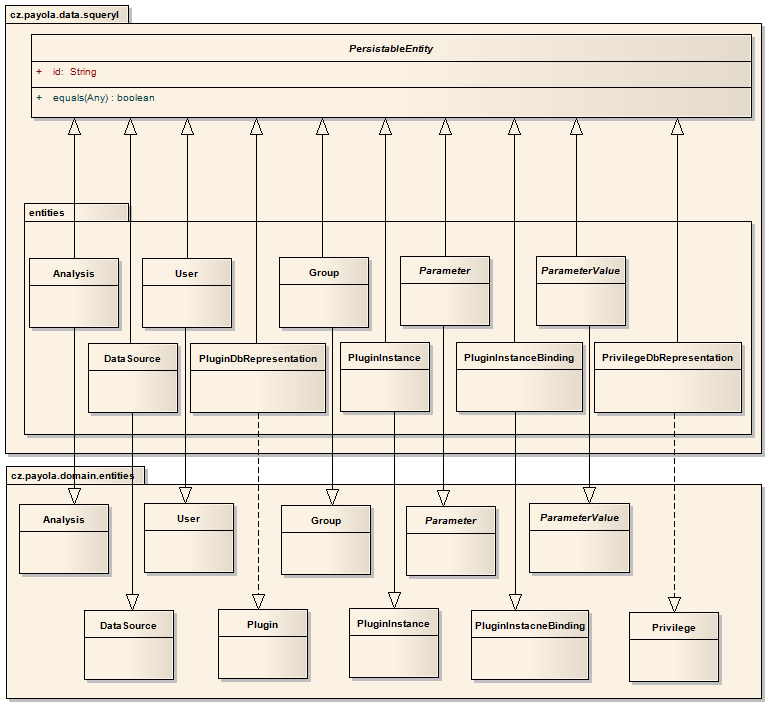
\includegraphics[width=140mm]{img/data_entities.png}
	\caption{The data access is~divided into~3 layers. The~first one, which is~a part of
	the common package defines entities and relations between them (not in~the figure ---
	see Figure~\ref{fig:packages-structure}).
	The second one is~a part of~the domain package. It~defines basic business logic.
	The last one has its own package --- data. It~binds the~others with a~concrete DAL
	implementation, in~this case with the~Squeryl ORM. ~\cite{payola:dg}}
	\label{fig:3-layers}
\end{figure}

The second reason is~that the~Payola data access layer is~consisted of~three different sublayers
(Figure~\ref{fig:3-layers}) and 
due to~the utilization of~the Squeryl ORM framework~\cite{squeryl} it~would be~a very difficult 
task to~try and modify the~existing database structure. In~the list of~the future changes of~the Payola framework there is~a thought for a~replacement of~the underlying ORM framework
and respectively for a~heavy refactoring of~the data access layer.

Therefore, we~have decided to~focus on~the task and implement the~feature with 
as little modifications to~the Payola framework as~possible. In~fact, the~used adjustment is
kept in~the socpe of~the newly added features and does not blemish the~rest of~the framework.

The implementation of~the plugin is~pretty straightforward since we~are 
taking advantage of~the Payola framework. The~Payola framework recognizes a
special subtype of~a \texttt{Plugin}, a~\texttt{SparqlQuery}. There is~a special 
reason for this as~a SPARQL query could be~executed on~a remote data source, 
e.g. a~SPARQL endpoint. A~series of~SPARQL queries could be~optimized into~a~single, more efficient query. Without such a~mechanism, the~framework would
have to~fetch all the~data from the~data source, transfer them to~the server 
where Payola is~running on, store them in~the memory (wrapped with
the Payola internal object representation) and pass it~to a~plugin. After that, the~graph would be~processed inefficiently within the~memory of~the Payola server with 
the JENA RDF toolkit consuming uselessly a~lot of~probably unnecessary computation time. See 
Figure~\ref{fig:plugin-hierarchy} to~see the~whole plugins’ hierarchy.


\begin{figure}
	\centering
	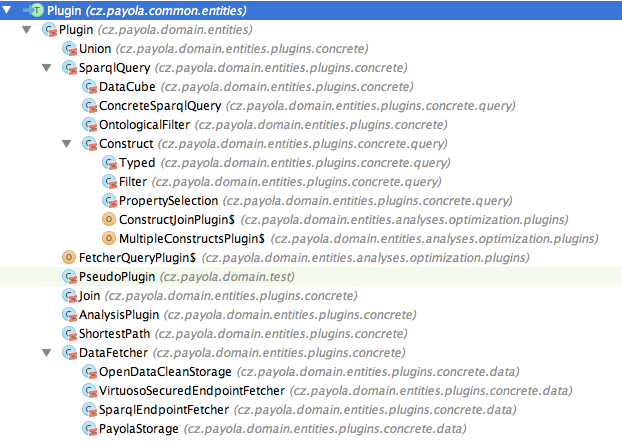
\includegraphics[width=100mm]{img/plugin-hierarchy.png}
	\caption{Payola plugin hierarchy. Notice the~SparqlQuery class.}
	\label{fig:plugin-hierarchy}
\end{figure}

Moreover, the~Payola framework restricts the~use of~a non--SPARQL--query 
in the~analytical pipeline right after the~data fetcher plugin. That is~done in~order to~avoid 
the aforementioned performance difficulties. There is~one restriction regarding our plugin if~we
were to~derive it~from the~\texttt{SparqlQuery} class. The~complete behaviour of~the plugin needs to~be expressed by~a single SPARQL query. Fortunately, such a~constraint does 
comply with what we~need in~order to~implement the~proposed system. That also means
that the~existing Payola query optimizer will engage and 
will make the~plugin execution faster. Therefore, the~system will again 
benefit from the~integration with the~Payola framework.

The plugin will load the~stored query from the~database and pass it~to the~evaluation framework, which will handle the~rest.

\subsection{Obtaining the~transformation pattern}
The more complicated task still awaits us. We~need to~implement an~interface, 
which will obtain the~transformation pattern from the~user. The~implementation 
builds up~on what we~have learnt of~the pattern in~Chapter~\ref{ch:proposal}.
The best way is~to simulate the~approach we~used for getting the~formal expression of~the transformation pattern
(see Section~\ref{sec:pattern-definition}).

We have already stated that we~are about to~implement a~user interface, which 
will allow the~user to~select the~pattern based on~the Tabulator's (Section~\ref{sec:rw:tabulator})
query--by--example principle. But to~do that, we~need to~introduce a~lot of~new 
features into~the~Payola framework.

\subsubsection{Analysis preview}
In order to~enable the~user to~choose a~pattern by~an example, we~need to~offer them a~preview
of the~given dataset. The~dataset serves as~an input graph of~the mapping process. 
We have decided to~make the~proposed system a~part of~the analytical 
pipeline, which brings on~some interesting and unexpected complications.

Mainly, the~dataset may come from any point of~the analytical pipeline execution. In~fact, we~need the~evaluation framework to~give us~a partial result. We~need the~analyzer to~process the~pipeline and at~some point, to~take an~input of~the 
inserted Data Cube Vocabulary Plugin instance and send it~to us~as a~result. 
Moreover, only a~part of~the pipeline could be~used to~make a~preview. For instance, if~had an~analysis
based on~extracting the~data from several different data sources, 
let us~say 4, those 4 fetching processes would run collaterally regardless of~the 
fact that the~DCV plugin is~a part of~one of~them. We~will throw away the~results of~the rest. It~is shown in~Figure~\ref{fig:dcv-preview-useful}.

\begin{figure}
	\centering
	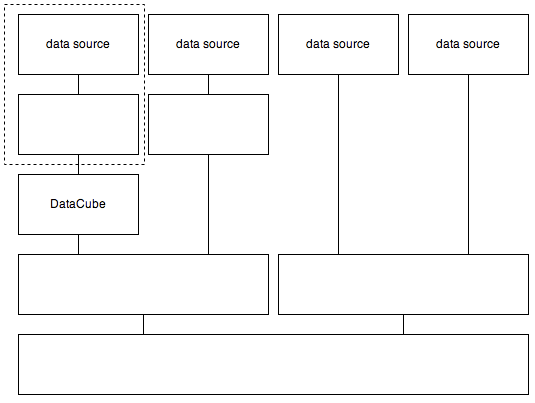
\includegraphics[width=100mm]{img/dcv-preview-useful.png}
	\caption{Making a~preview for the~Data Cube Vocabulary plugin. Only the~plugins in
	the dashed box are relevant. The~rest of~the analytical pipeline is~not.}
	\label{fig:dcv-preview-useful}
\end{figure}

It brings on~not only a~technical complication, it~also rises a~performance 
question. The~analytical pipeline may take a~lot of~time to~be processed.

That is~why we~had to~introduce a~mechanism, which, in~the right moment, 
extracts a~proper sub--pipeline. If~the reader looks closer on~Figure~\ref{fig:example-analysis} they learn that the~pipeline is,
in the~reverse topological order, 
a tree (as known from the~graph theory). Every instance has 
one output. Every output is~connected to~an input of~a successor (if present, if~not it~is an~output
of the~whole pipeline). Therefore, it~is easy to~traverse the~tree and select a~subtree, which precedes the~Data Cube Vocabulary plugin instance.

Such a~tree is~then used in~the background without the~knowledge of~the user to~create a~completely new analytical pipeline. When this step is~complete, such a~pipeline can 
be executed by~a standard pipeline evaluator. That is~because the~result of~the whole 
newly created pipeline is~the dataset we~make the~preview from.
See an~example of~such a~pipeline in~Figure~\ref{fig:dcv-extraction}.

\begin{figure}
	\centering
	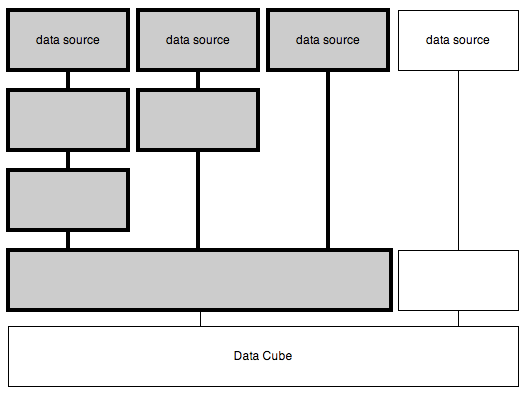
\includegraphics[width=100mm]{img/dcv-extraction.png}
	\caption{Making a~preview for the~Data Cube Vocabulary plugin. The~highlighted
	plugins are required to~be evaluated and becomes a~part of~a sub--pipeline created
	in the~background.}
	\label{fig:dcv-extraction}
\end{figure}

Nonetheless, what remains is~a potential performance problem, which is~partially given 
by features provided by~the Payola framework. The~result of~executing an~analytical pipeline could become eventually a~very huge dataset. A~dataset so~large that it~may not fit into~the~memory of~the user's computer. That is~a 
limiting factor, since the~visualisation is~performed fully on~the client--side. 
It makes no~difference whether it~is a~table or~a graph rendered into~the~canvas HTML element.

In order to~solve this problem in~the Payola framework, a~larger milestone is~planned. The~results need to~be cached on~the server hosting Payola.
Such an~approach could be~seen in~the case of~the project 
Explorator (section~\ref{sec:rw:explorator}) project, which implemented a~local cache
while utilizing the~tool SESAME~\cite{sesame}. It~is planned to~introduce a~new 
subtype of~the~\texttt{Graph} trait, ~\texttt{PersistentGraph}, which would be~cached on~the Payola server in~order to~enable techniques like pagination, 
exploration in~the analytical mode, etc. Since this requires also a~huge 
modification to~the existing visualizers but is~not a~goal of~this thesis, we~will 
not realize this plan. However we~will implement the~preview in~a way that will 
automatically take advantage of~the modifications when they are done.

This still leaves us~with the~problem of~a huge results dataset. Therefore, we~decided to~make use of~the~\texttt{LIMIT} SPARQL query statement, which will 
enforce the~results to~be reasonably large. This could be~done by~extending the~previously extracted sub--pipeline with appending a~plugin that 
will limit the~number of~the results of~the analytical
pipeline evaluation (see Figure~\ref{fig:dcv-extraction-limit}). Therefore, we~introduced another completely new plugin -- \texttt{Limit}.

\begin{figure}
	\centering
	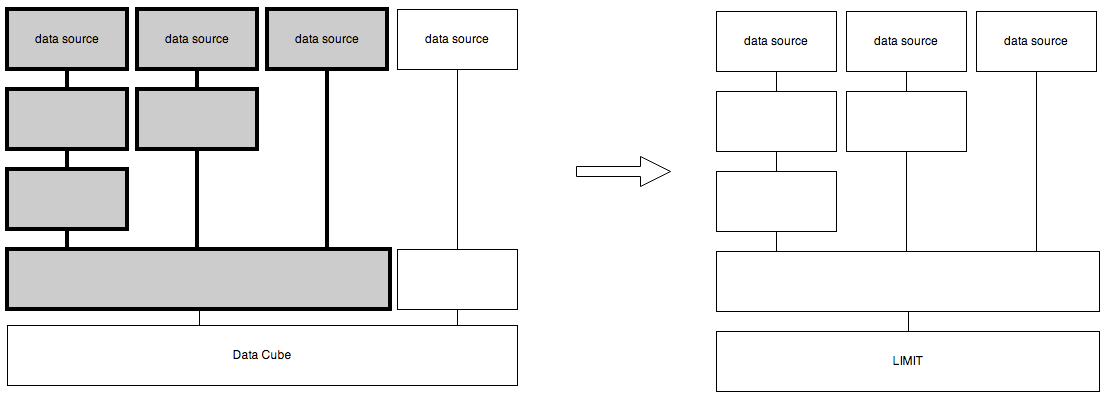
\includegraphics[width=140mm]{img/dcv-extraction-limit.png}
	\caption{Making a~preview for the~Data Cube Vocabulary plugin. An~instance of
	SparqlQuery plugin representing a~LIMIT statement is~added.}
	\label{fig:dcv-extraction-limit}
\end{figure}

Unfortunately, that brings a~completely new problem. By~limiting the~size of~the result, it~is possible that some important vertices might get excluded from the~preview.
And there is~no way of~telling, which vertices could be~important to~the user. Therefore, we~made the~size of~the preview to~be a~variable that could be~changed before making the~preview and 
selecting the~transformation pattern. Of~course, the~better approach would be~to 
insert the~plugin into~such an~execution point of~the pipeline that it~would 
work with data as~small as~possible. In~other words, we~should use an~analysis 
to compensate a~large size of~the original dataset, if~possible.



\subsubsection{Obtaining the~pattern}
Hopefully, it~is now fully understood what is~required to~be done before a~preview 
is made so~we can move onto the~description of~the way of~obtaining the~pattern 
from the~user. Moreover, we~will describe, which components and why have been 
modified or~newly implemented.

\begin{sloppypar}
We take advantage of~the previously presented approach (the query--by--example), which we~consider to~be the~best for the~user. Firstly, the~user is~asked to~mark a~vertex that represents
the first component of~the associated Data Cube Vocabulary data structure 
definition. Since the~only criteria we~set is~that the~pattern needs to~be a~connected graph at~any time, it~is sufficient to~select only a~single vertex.
Of course, the~user might consider selecting a~more complicated pattern with keeping in~mind the~\emph{reference vertex} concept mentioned in~the proposal (Chapter~\ref{ch:proposal}).
\end{sloppypar}

If we~enable the~user to~extend the~pattern not only by~adding a~vertex, 
which has an~incoming edge from one of~the already added vertices, but also by~adding 
a vertex, which has an~outgoing edge into~one of~the already added vertices, 
the user is~capable of~building a~complicated pattern in~a way compatible with a~natural thinking process.
They will select the
important vertex \emph{accidentally} while extending the~pattern in~order to~select another. Therefore, the~only restriction 
applied in~the vertex selection mode is~that we~prevent the~user from selecting 
a non--related vertex (more accurately a~vertex, which would break the~connected 
graph invariant).

The selection process is~made to~be as~simple as~possible. We~will describe the~user interface in~the following text more deeply.

\subsection{User interface}
The basics of~the user interface come out of~the architecture of~the Payola 
framework. We~need to~make the~plugin as~simple as~possible for the~user. But we~also need to~keep it~aligned with the~design of~the Payola framework. In~order to~make the~reader understand the~following text, we~need to~dive a~bit into~the~architecture of~the Payola application.

As stated before, Payola is~a web application. Its implementation is~based on~the MVC 
design pattern. Nowadays, that is~a usual approach to~a web application. However, it~is not that usual 
to acquire a~stance to~the utilization of~a design pattern on~the client--side. The~Payola team has decided to~use the~MVC pattern there as~well and due to~the presence of~the s2js compiler, the~client--side is~also being developed in~the Scala programming language.

Therefore a~majority of~pages produced by~the Payola application is~delivered 
in two different parts. The~layout of~a page and a~placeholder for the~client 
side application is~rendered on~the server while utilizing the~subsystems of~the 
Play Framework 2.x. The~placeholder is~then provided to~a JavaScript application,
which is~referenced from the~rendered layout. The~utilization of~the s2js compiler and
the custom RPC gateway (which translates JSON calls into~method invocation and serializes its results
back to~the client), prevents code duplication and makes the~development process more transparent.

Therefore, every client--side application can avoid becoming a~confusing piece of~a
spaghetti code and utilize the~MVC pattern. A~crucial feature is~the RPC 
mechanism that, hand in~hand with the~s2js compiler brings a~way of~transparent 
client--server communication.

The analytical pipeline editor is~one of~those client--side MVC applications. We~are interested specifically in~this one since we~require for it~to be~able to~work 
with our newly introduced Data Cube Vocabulary analytical plugin.

Until now, the~pipeline editor applied a~unified approach for rendering the~layout of~the pipeline. Every plugin was rendered while using a~generic 
renderer, which determined the~appearance of~the plugin based on~its metadata. An~example of~such a~rendered pipeline could be~seen in
Figure~\ref{fig:example-analysis-editable}. The~reader can see a~rendered title, based on~the name of~the plugin and a~parameter form. The~form is~based on~the type of~the 
corresponding parameters. A~\texttt{string} parameter gets rendered as~an input or~a textarea based on
an additional flag \texttt{isMultiline}, which determines whether the~value can be~spread into~multiple lines.
A \texttt{int} or~\texttt{float} parameter is~also rendered as~an input field. A~\texttt{boolean} parameter 
is rendered as~a checkbox.

\begin{figure}
  \centering
    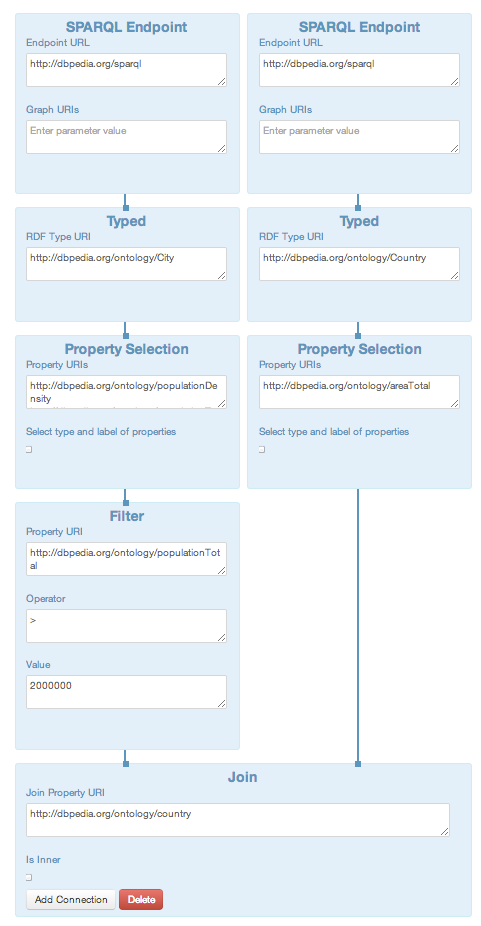
\includegraphics[width=100mm]{img/editable-analysis.png}
  \caption{An example of~an editable analysis (retrieving a~list of~cities with a~certain population size).}
  \label{fig:example-analysis-editable}
\end{figure}

Since we~would like to~provide the~ability to~select a~pattern, we~need to~introduce a~completely new approach. To~keep it~generic, we~start with the~modification of~the parameters subsystem. We~would like to~introduce a~new type 
of parameter, a~\texttt{pattern}. Since the~data access layer of~Payola is~very 
difficult to~modify, we~use a~less obtrusive approach. A~pattern results in~a 
SPARQL query, which is~a string. Therefore, we~add a~flag to~the string 
parameter, called~\texttt{isPattern}, which the~system will take advantage of. It~is based on~the same unobtrusive principle as~the \texttt{isMultiline} flag.

Another problem comes out of~the fact that a~plugin has as~many parameters as~the data structure definition has components and we~utilize just the~first one 
to store the~query. That also means that we~need to~render the~representation 
of the~plugin in~a slightly different way. At~the time of~implementing this 
thesis, the~same requirement came up~from two other developers who integrate their 
tools with Payola. Therefore, we~introduced a~mechanism, which solves the~problem of~loading custom plugin renderers.

We introduce a~dynamic plugin instance renderer loader for an~analysis editor. 
Based on~the plugin classname, it~tries to~load a~custom override of~the default 
renderer. It~enhances the~extensibility of~Payola. Until now, it~was not 
possible to~override the~visualization of~a plugin instance within the~editor. The~user was able to~upload a~custom analytical plugin, but they were not capable of~affecting its
appearance in~the editor.

\begin{sloppypar}
With our loader, the~user is~able to~define a~custom renderer derived from 
one of~the \texttt{ReadOnlyPluginInstanceView} and \texttt{EditablePluginInstanceView} 
classes. The~name of~the override is~precisely given. It~is required to~match one 
of the~following patterns: \texttt{{classname}PluginInstanceView},
\texttt{{classname}EditablePluginInstanceView}. The~implementation is~required to
be declared within the~\texttt{cz.payola.web.client.views.entity.plugins.custom} package.
\end{sloppypar}

\begin{sloppypar}
The editor was altered so~that it~does not create renderer instances itself. It~uses a~newly introduced \texttt{PluginInstanceViewFactory}. This 
factory is~responsible for creating a~proper instance. Based on~the given plugin 
classname it~calls a~dependency package manager. The~manager is~a part of~the 
s2js compiler and it~provides a~JavaScript implementation of~the required class
with all the~necessary dependencies. Therefore the~factory calls the~manager and 
requests an~implementation of~a specified override. If~it exists, the~manager 
returns its implementation. If~it does not, it~returns an~empty string. After 
that, the~factory tries to~make an~instance of~the override. If~it succeeds, an~instance of~the override renderer is~created. If~it fails, it~returns an~instance of~a generic renderer. 
\end{sloppypar}
 
Our custom implementation of~the Data Cube Vocabulary plugin renderer results 
in a~form shown in~Figure~\ref{fig:DCV-plugin-view}. First of~all, it~enables the~user to~select the~pattern. Clicking the~Preview button starts the~process of~making a
sub--pipeline, evaluating it~and rendering a~preview. It~also opens a~pattern--selection
dialog, which we~introduce later. The~second provided field enables the~user to~specify how large should 
the pattern--selection preview be. We~have already presented the~reason behind this 
a few paragraphs above.

\begin{figure}
	\centering
	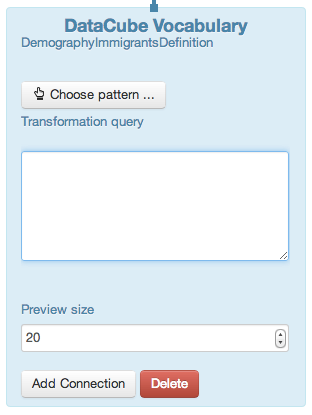
\includegraphics[width=60mm]{img/custom-dcv-piv.png}
	\caption{Data Cube Vocabulary plugin instance custom view.}
	\label{fig:DCV-plugin-view}
\end{figure}

The last part of~the UI~is the~pattern selection dialog. After the~user clicks 
on the~button of~the rendered plugin, the~application extracts a~sub--pipeline, 
which is~relevant to~the preview. Such a~pipeline is~executed
automatically. When the~pipeline evaluation is~done, the~application opens a~new 
dialog, which gives the~user the~opportunity to~select the~transformation 
pattern. With every step, the~user is~presented with a~label and/or a~URI of~the 
matching DCV component based on~what is~available. An~example of~a pattern 
selection is~shown in~Figure~\ref{fig:pattern-selection} (some additional details are provided
in Section~\ref{sec:pattern-definition}
and in~figures~\ref{fig:pattern-selection} and~\ref{fig:pattern-enhancement}).
With a~single click 
the user includes a~vertex into~a~constructed pattern. A~double--click 
has it~representing a~currently processed component. We~also had to~modify the~visualization algorithm to~avoid collapsing literal vertices into~an~info table. 
We need the~literals to~remain visualized in~order to~be selectable.

\begin{figure}
	\centering
	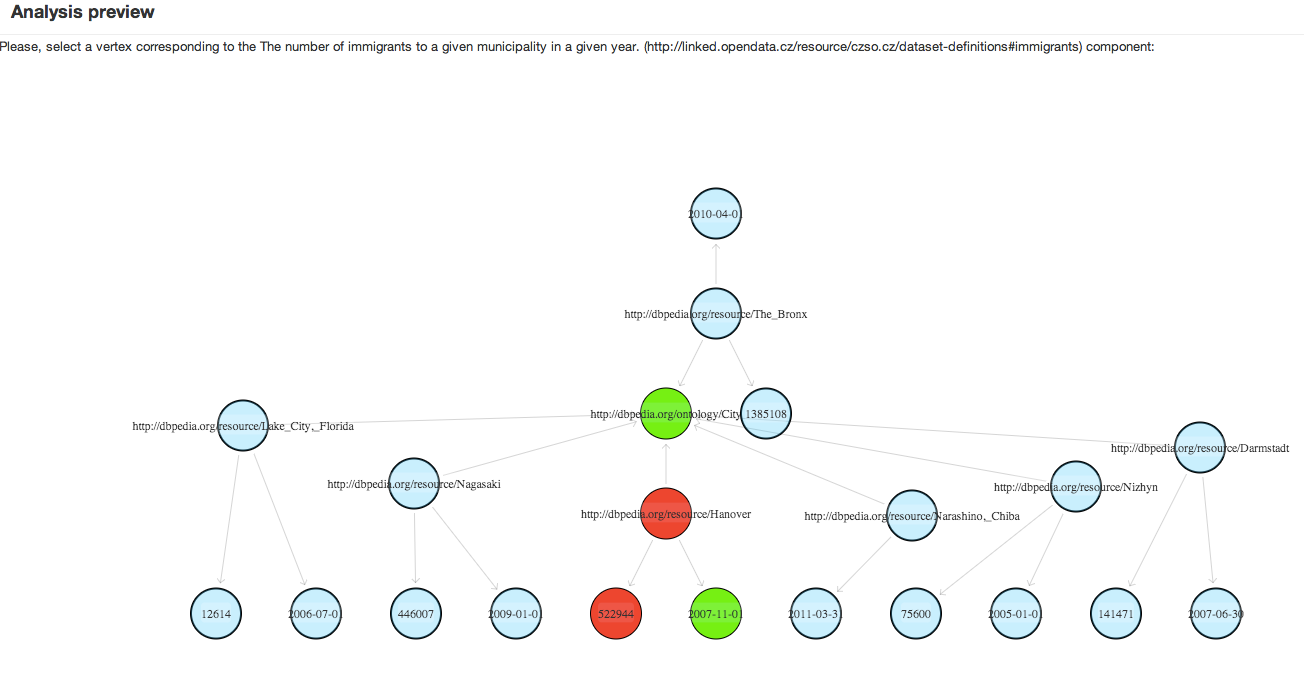
\includegraphics[width=140mm]{img/pattern-selection.png}
	\caption{An example of~a pattern selection.}
	\label{fig:pattern-selection}
\end{figure}

\section{Visualisers}
As stated in~Chapter~\ref{ch:proposal}, we~have decided to~implement two 
different visualization plugins for Payola. All the~presented 
visualizers are configurable by~specifying a~Data Cube Vocabulary.
As in~the case of~the rest of~the 
system, the~implementation of~the visualization plugins will be~influenced 
by the~architecture and features of~the Payola framework as~well.

The feature that is~lacking the~most  is~a sophisticated faceted browsing. All the~presented plugins 
implement offered filters only on~the client--side, therefore all the~data needs 
to be~loaded within the~memory of~the user’s computer. As~described before, Payola 
needs a~series of~modifications in~order to~work effectively with larger 
datasets, hence a~client--side--only visualization is~the only one currently making sense.

To make them able to~work with the~Data Cube vocabularies, we~had to~append 
definitions of~those vocabularies into~the~result of~the mapping process. The~visualizer is~then able to~acquire them and take advantage of~them. For instance 
while building a~user interface.

\subsection{TimeHeatmap}
In order to~deliver the~TimeHeatmap visualizer, we~took advantage of~an existing 
map library. We~chose to~integrate a~visualization based on~Google Maps API. We~decided to~do so~for several reasons. One of~them is~an easy use of~the API and that it~allows us~to
create an~eye--catching visualization in~a short 
time. Google is~known for its high--quality map imagery and due to~its 
infrastructure also for a~reliable delivery. The~API also offers the~ability to~create a~heatmap layer.

But the~heatmap layer itself is~not enough. In~order to~support the~time 
dimension, we~had to~come up~with a~way of~visualizing time entries. The~interface is~built with the~following idea in~mind. Let us~imagine an~example of~population size data (see Figure~\ref{fig:impl-pop-ex}).

\begin{table}
  \begin{center}
\begin{tabular}{l|l|l}
  City & Population size & Year \\ \hline
  Prague   &    1000000   &   2010 \\
  Prague   &    1100000   &   2011 \\
  Prague   &    1200000   &   2011 \\
  Liberec   &    100000    &  2010 \\
  Liberec   &    110000    &  2011 \\
  Liberec    &   112000    &  2012
\end{tabular}
\caption{Population size example}
\label{fig:impl-pop-ex}
  \end{center}
\end{table}

It is~more constructive to~visualize such a~dataset year--by--year. Grouped values are 
not very attractive no~matter what aggregation is~applied. The~most useful 
approach is~to enable the~user to~make a~slice based on~the year and visualize a~heatmap for the~selected year.

Therefore, we~wrap the~map with a~custom control. It~contains a~list of~years 
detected in~the dataset. The~user is~able to~select an~arbitrary subset of~years. The~visualizer shows and hides a~corresponding layer based on~what is~selected. 

In order to~deliver an~easy--to--use visualizer, we~decided to~ignore GPS 
data and employ places names. With the~integration of~the Geocoder library of~a 
colleague of~ours, Matej Snoha, the~visualizer is~now able to~translate the~names of~the places to~GPS coordinates and place them into~the~map. The~library takes 
advantage of~a locally installed application Gisgraphy. The~installation is~maintained by~the author of~the used library.

We tried to~make the~visualization as~easy as~possible, therefore we~decided to~exert the
URI resource itself. It~usually contains the~name of~the place 
in a~way, which is~convertible into~a~form recognized by~the Gisgraphy 
application. For instance, \texttt{http://dbpedia.org/page/Brasserie\_Du\_Bocq} 
can be~converted into~Brasserie du~Bocq very easily.

An example of~such a~visualisation will be~presented in~Chapter~\ref{ch:experiments}.

\subsection{Universal Data Cube Vocabulary}
We decided to~offer a~basic set of~usual statistical visualisations. As~stated 
in Chapter~\ref{ch:proposal}, we~achieve that by~giving the~user the~ability to~slice the~dataset. We~need them to~fix values of~$n-1$ dimensions in~order to~transform the~dataset into~a~two--dimensional one (1 dimension + 1 measure).

We took advantage of~the chart library Flot~\cite{flot} and prepared a~visualizer, which allows the~user to~create bar or~pie charts. It~comes out from the~proposal shown in~Figure~\ref{fig:dcv-universal}. By~applying filters, the~user slices the~dataset.

It supports multiple dimensions, attributes and even measures. It~is 
configurable by~a Data Cube Vocabulary. We~require the~user to~specify a~dimension that gets to~be used on~x--axis of~a bar chart (or defined groups in~a 
pie chart). Based on~filters, the~visualizer groups DCV measures by~the specified 
dimension (aggregated by~applying sum function). In~case of~a bar chart, multiple measures are 
displayed as~groups of~columns.

We present an~example of~a visualization made by~this plugin in~Chapter~\ref{ch:experiments}.

\section{Payola improvements}
In order to~make the~added value of~the Payola application integrated with the~proposed system even higher, we~decided to~implement also some other
improvements. Mostly in~order to~enhance the~user experience. Some of~the changes
had also brought completely new features and possibilities. We~will mention 
these modifications briefly. Since they are of~a rather technical character 
than scientific, we~will make the~corresponding analyses a~part of~the 
implementation reports in~order to~make the~text consistent for the~reader.

\subsection{LodVis integration}
While writing the~review of~the tool LodVis (see Section ~\ref{rw:lodvis}), 
we have discovered, that the~provided features are very conducive though completely 
missing in~Payola. The~application does not offer an~overview of~a dataset in~order 
to help discover the~most used concepts.

Since we~want the~user to~know their dataset before choosing the~pattern in~the 
preview, we~find this tool very interesting. It~may help the~user to~locate the~statistical subset of~the data. Therefore, we~discovered a~simple way of~implementing a~plain kind of~interaction between Payola and LodVis.

\subsubsection{Visualising Payola data sources in~LodVis}
The first part is~introducing a~way of~allowing the~user to~visualize a~dataset in~the scope of~the LodVis application. That is~done by~utilizing a~simple REST API. We~only create a~link, which is~inserted wherever we~consider it~relevant. The~user can click on~the link in~order to~switch to~LodVis,
which handles the~rest. We~utilize a~simple URL pattern:

{  \scriptsize
\begin{verbatim}
http://lodvisualization.appspot.com/?graphUri={graph-uri}&endpointUri={endpoint-uri}
\end{verbatim}
}

The pattern has only two parameters. The~first one, the~\texttt{graph-uri} 
designates the~URI of~the graph we~want LodVis to~visualise. This parameter is~not mandatory. The~second parameter, \texttt{endpoint-uri} is~required and it~tells the~LodVis application, where to~fetch the~data from. It~is not possible 
to visualize results of~an analysis in~LodVis. An~example of~this could
be seen in~Figure~\ref{fig:lodvis-int}.

\begin{figure}
	\centering
	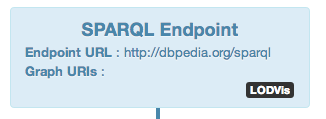
\includegraphics[width=55mm]{img/lodvis-int.png}
	\caption{LodVis integration link in~a visualization of~an analytical pipeline.}
	\label{fig:lodvis-int}
\end{figure}


\subsubsection{Visualising Payola data sources in~LodVis}
With cooperation of~the LodVis team, we~have also implemented a~reverse 
mechanism --- an~API, which allows the~user of~the LodVis application to~browse a~dataset in~the scope of~the Payola application. To~make it~easy for the~LodVis 
team to~integrate a~link to~the Payola application, we~prepared an~API very 
similar to~theirs. The~URL pattern is~very similar:

{  \scriptsize
\begin{verbatim}
http://live.payola.cz/visualize?endpointUri={endpoint-uri}&graphUri={graph-uri}
\end{verbatim}
}

In addition, we~support referencing a~list of~graph URIs separated by~a comma. Since 
we wanted to~avoid any difficulties arising from passing a~URI in~an 
URL, we~decided to~have the~parameters encoded with the~Base64 algorithm.

The only problem was, that Payola was not able to~visualize a~dataset not registered
within its database. Therefore, when somebody accesses the~URL, the~application takes the~parameters and creates an~anonymous analyzer 
pipeline. The~only plugin in~the pipeline is~a data source specified by~the 
passed parameters. By~evaluating such a~pipeline, the~user is~able to~visualize 
the neighbourhood of~the vertex in~the given dataset. The~vertex is~chosen by~the 
SPARQL endpoint backend, e.g. OpenLink Virutoso~\cite{virtuoso}.

To allow an~anonymous user to~modify the~pipeline, we~also set a~cookie with an~authorization token to~their browser. When logged into~ 
Payola a~user with such a~token can overtake the~ownership of~the pipeline and 
fully modify it.

\subsection{Secured endpoints}
What was also lacking was the~support for password--guarded SPARQL endpoints. 
It is~a natural matter, that a~company would like to~keep its statistics 
non--public, but they might wish to~analyze and visualize them. Therefore, we~have decided to~introduce a~support for secured endpoints.

Since every SPARQL endpoint may have different possible solutions, we~have 
introduced a~support for only one specific engine. We~chose the~most
used OpenLink Virutoso~\cite{virtuoso}.
It takes advantage of~the Digest HTTP authentication as~introduced in~the 
RFC~2617~\cite{rfc-2617}. Therefore, we~had to~include the~Apache HTTP commons 
library~\cite{apache-http-commons}. It~was also necessary to~introduce a~new 
subtype of~\texttt{string} parameter --- \texttt{password}. That was done as~before (remember the~\texttt{isMultiline} or~the \texttt{isPattern} flag) by~adding a~new flag.

One can see a~visualization of~the described plugin in~Figure~\ref{fig:secured-ds}. 

\begin{figure}
	\centering
	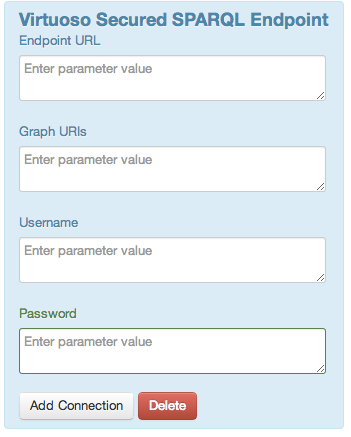
\includegraphics[width=55mm]{img/secured.png}
	\caption{One may simply include an~instance of~Virtuoso Secured SPARQL Endpoint plugin instead
	of an~instance of~the generic SPARQL Endpoint plugin.}
	\label{fig:secured-ds}
\end{figure}

\subsection{Analytical pipeline reuse}
During the~period of~writing this thesis Payola has undertaken a~user test. One 
of the~significant results of~the test was that the~users wished to~modify the
analyses of~others. At~least, they would like to~reference an~analysis of~another user within their own. That also fits into~analyzing statistical data --- 
a company provides an~analysis and presents its statistics while somebody else 
whishes to~process them and apply DCV. That is~why two different features 
were added.

\subsubsection{Clone and edit}
The first one is~less powerful. It~enables the~user to~clone an~analysis of~another user. After doing that, they get a~newly created analysis owned by~them. Therefore, they are in~a full control of~the analysis and may modify it~in 
any way they want.

We were required to~enhance the~capabilities of~the application in~order to~support cloning a~plugin instance. We~also had to~clone bindings from an~existing analytical pipeline and translate the~identifiers of~the cloned plugin 
instances in~order to~keep the~bindings working.

The most difficult part was, unfortunately, to~find a~way of~storing the~cloned 
analysis, because the~data access layer was not prepared for that. That is~why
the persistence of~the cloned analysis had to~be split into~several steps and may take a~bit longer than expected.

As a~result the~user is~presented with a~inconspicuous button as~shown in~Figure~\ref{fig:clone-button}.

\begin{figure}
	\centering
	
\includegraphics[width=100mm]{img/clone-button.png}
	\caption{A clone button.}
	\label{fig:clone-button}
\end{figure}

\subsubsection{Inner analyses}
Much powerful feature is~enabling the~user to~reference an~existing analysis in~another one. We~introduced a~fake analytical plugin with no~implementation at~all. It~allows the~user to~insert a~reference to~an existing analysis instead 
of specifying a~data source. As~the inserted analysis generates a~graph, 
it is~hence a~graph generator and might be~considered a~data source.

Of course, we~had to~find a~way of~implementing such a~feature without 
making huge modifications of~the evaluation framework. That is~why the~plugin 
has no~implementation at~all. The~trick is~that before starting an~analysis 
evaluation we~walk through the~analysis and make some changes. The~idea is~very 
simple. We~examine the~analysis and replace each instance of~the fake plugin 
with all the~plugins from the~referenced analysis. We~call such a~process an~\emph{analysis expansion}.

To make the~feature even more sophisticated we~made a~special user interface to~enable them to~parametrize an~inner analysis. When inserting an~analysis into~another, the~user is~able to~click the~names of~parameters of~plugin instances 
in the~inner analysis in~order to~promote them to~\emph{analysis parameters}.

That is~why we~took an~advantage of~what we~have learnt while implementing the~core of~this thesis and created a~special plugin for each inner analysis. That 
makes it~possible for the~plugin to~have a~variable parameters count. As~a result the~user creates a~new shareable plugin. Such a~plugin is~also promoted to~be a~new 
data source available at~any time in~the future.

Moreover, we~gave the~user a~tool for a~simple parametrization of~an existing analysis. 
They do~not need to~extend the~analysis with other steps. They may simply take 
advantage of~the new feature to~ease their work.

\begin{figure}
	\centering
	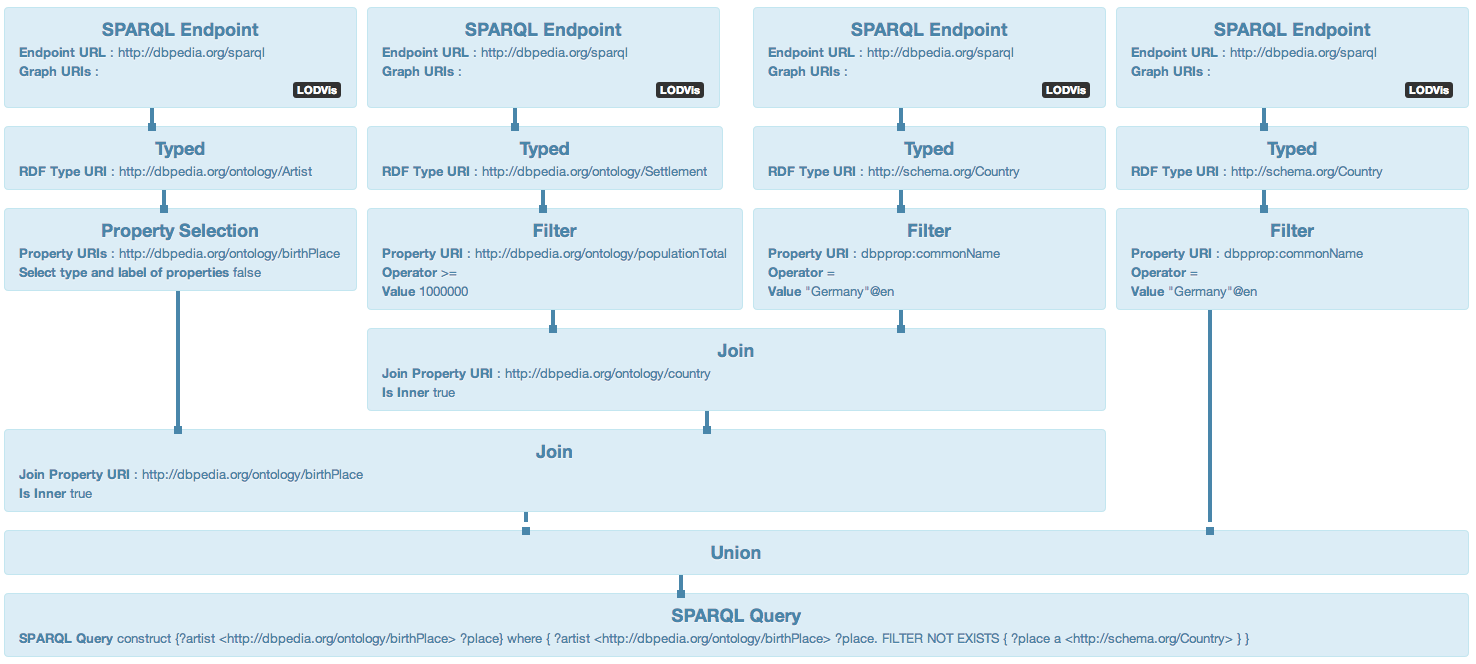
\includegraphics[width=140mm]{img/inner-example.png}
	\caption{A great example of~an analysis that can benefit from inner analyses. Notice the
	two rightmost branches of~the analytical pipeline. They are the~same. By~making
	an inner analysis we~can at~least convert the~analysis into~a~pipeline shown in~	Figure~\ref{fig:inner-example-simpler}}.
	\label{fig:inner-example}
\end{figure}

\begin{figure}
	\centering
	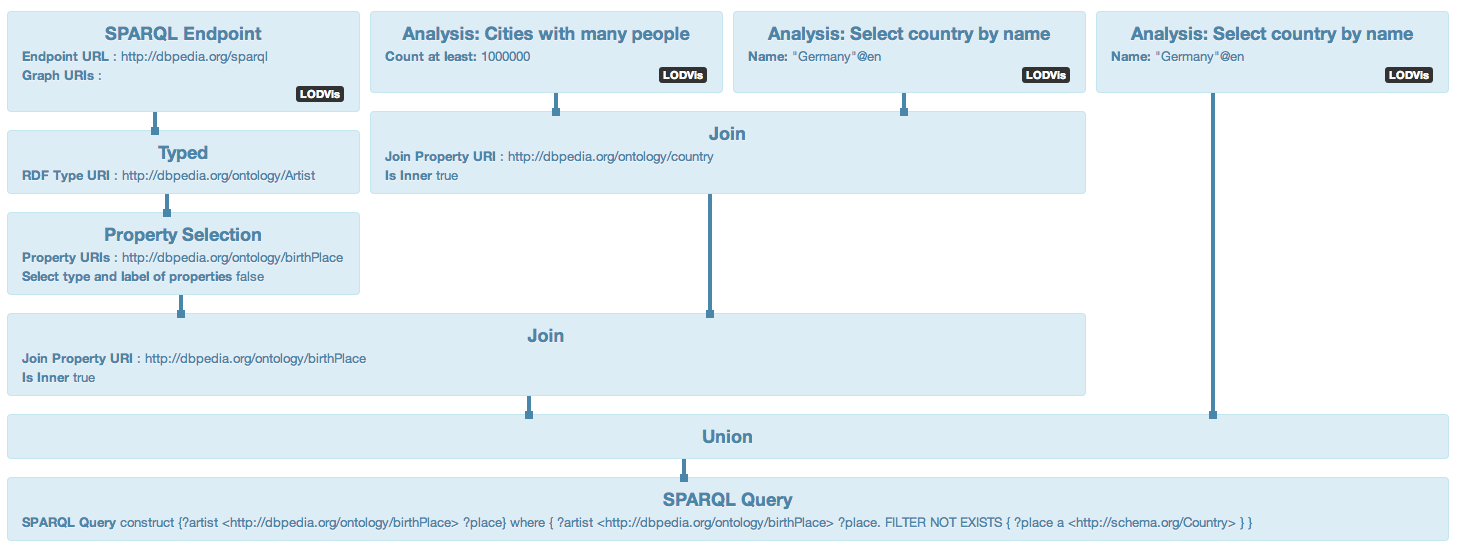
\includegraphics[width=140mm]{img/inner-example-simpler.png}
	\caption{An example of~simplifying an~analysis while utilizing inner analyses.}.
	\label{fig:inner-example-simpler}
\end{figure}

\subsection{Data Source browser permalinks}
Another minor change was done within the~scope of~the data source browser.
We introduced a~mechanism, which enables the~user to~send a~link to~a current 
state of~the triple table data source browser. It~detects the~specified URI in~the URL and fetches an~initial vertex based on~that. The~original behaviour delegates 
the decision on~an underlying engine of~the queried data source. We~simply add a~location hash to~the URL that makes the~permalink available in~the address bar 
of the~user's browser. The~implementation was extended with an~onload event 
handler, which looks for the~location hash and reacts to~it.

\subsection{Limit plugin}
In order to~bring a~better performance and user experience to~the DataCube plugin
preview mechanism, we~had to~implement a~completely new plugin. It~is derived 
from the~\texttt{ConstructQuery} class in~order to~allow some optimalizations. 
We needed to~modify the~\texttt{DataFetcher} plugin and introduce new 
optimalization phases to~increase the~speed of~the most common cases of~dataset 
preview. For instance, we~merge a~\texttt{DataFetcher} plugin followed by~\texttt{Typed} and \texttt{Filter}, terminated with the~\texttt{Limit} plugin 
into a~single SPARQL query. We~have also implemented a~phase which optimizes
the query in~the case we~combine a~common SPARQL query with the~\texttt{Limit} plugin.

\chapter{Experiments}
\label{ch:experiments}

In this chapter, we~would like to~demonstrate the~abilities of~the implemented system. We
experimented with a~variety of~datasets and will use some of~them to~show how 
the system works. We~will also present how the~implemented visualizers work on~an example of~real--world data.

\section{DBPedia demography}
We used the~example of~the DBPedia demography throughout the~whole thesis. Now 
it is~time to~show how the~implemented system deals with such a~dataset. In~order to~start the~conversion, we~need to~have a~dataset (DBPedia) and a~vocabulary containing a~data structure definition. We~made a~custom vocabulary 
with a~definition as~shown in~Figure~\ref{fig:dcv-dbpedia-dsd}.

\begin{figure}
  \scriptsize
  \begin{verbatim}
@prefix rdf:     <http://www.w3.org/1999/02/22-rdf-syntax-ns#> .
@prefix rdfs:    <http://www.w3.org/2000/01/rdf-schema#> .
@prefix xsd:     <http://www.w3.org/2001/XMLSchema#> .

@prefix qb:              <http://purl.org/linked-data/cube#> .
@prefix sdmx:            <http://purl.org/linked-data/sdmx#> .
@prefix sdmx-concept:    <http://purl.org/linked-data/sdmx/2009/concept#> .
@prefix sdmx-dimension:  <http://purl.org/linked-data/sdmx/2009/dimension#> .
@prefix sdmx-measure:    <http://purl.org/linked-data/sdmx/2009/measure#> .


@prefix payola-dcv:   <http://datacube.payola.cz/dataset-definitions#> .

payola-dcv:PopulationSizeDefinition a~qb:DataStructureDefinition ;
  rdfs:label "The definition of~the DS~of a~dataset containing information about population size."@en ;
  # Dimensions
  qb:component [
    qb:dimension payola-dcv:location;
    qb:order 1 ;
    rdfs:label "The dimension representing populated location."
  ] ;
  qb:component [	
    qb:dimension payola-dcv:period;
    qb:order 2 ;
    rdfs:label "The dimension representing the~time of~the measurement."
  ] ;
  # Measure
  qb:component [
    qb:measure payola-dcv:populationSize;
    rdfs:label "The measure representing the~total count of~citizens."@en
  ] .
  # Attributes

payola-dcv:location a~rdf:Property, qb:DimensionProperty ;
  rdfs:label "reference location"@en ;
  qb:concept sdmx-concept:refArea .

payola-dcv:period a~rdf:Property, qb:DimensionProperty ;
  rdfs:label "reference period"@en ;
  qb:concept sdmx-concept:refPeriod .

payola-dcv:populationSize a~rdf:Property, qb:MeasureProperty ;
  rdfs:label "population at~the end of~the measured period"@en ;
  rdfs:subPropertyOf sdmx-measure:obsValue ;
  rdfs:range xsd:nonNegativeInteger ;
  qb:concept sdmx-concept:statPop .
  \end{verbatim}
  \caption{A custom Data Cube vocabulary containing a~data structure definition for population size.}
  \label{fig:dcv-dbpedia-dsd}
\end{figure}

\begin{sloppypar}
DBPedia is~based on~a very large dataset (about 400 million facts). Therefore we~need to~narrow down the~dataset a~lot in~order to~make a~meaningful data preview for 
the
pattern selection. We~briefly examined the~resource~\texttt{http://dbpedia.org/Prague} 
and learnt that it~is of~a type~\texttt{dbpedia-owl:City} and has two 
important properties -- \texttt{dbpedia-owl:populationTotal} and 
\texttt{dbpedia-owl:populationAsOf}. Hence, we~prepared an~analytical pipeline 
as shown in~Figure~\ref{fig:dbpedia-pop-anal}.
\end{sloppypar}

\begin{figure}
  \centering
  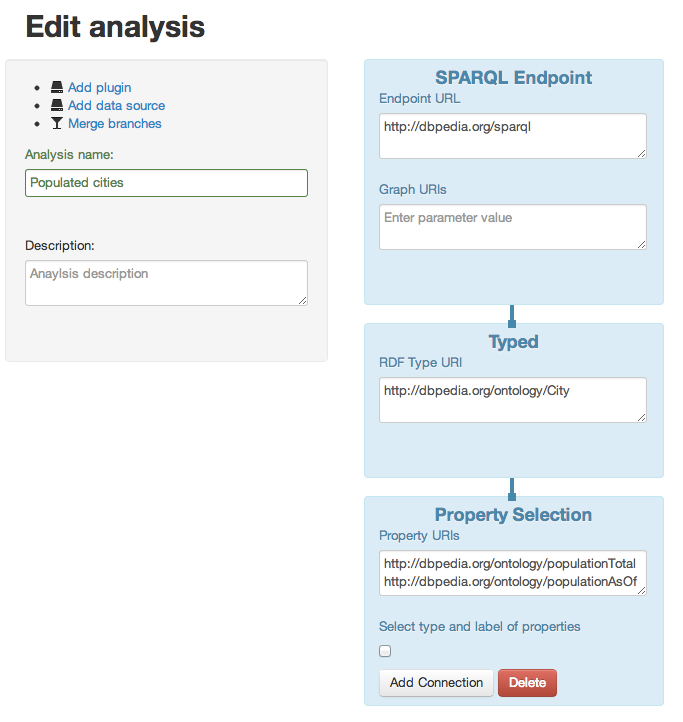
\includegraphics[width=100mm]{img/payola-exp-01-step1.png}
  \caption{An analytical pipeline made to~extract population data from the~DBPedia.}
  \label{fig:dbpedia-pop-anal}
\end{figure}

With the~preview size set to~20, the~preview is~shown as~pictured in~Figure~\ref{fig:payola-exp-01-preview}. In~this case, the~transformation pattern 
is very simple, as~shown in~Figure~\ref{fig:payola-exp-01-selection}. As~a 
result, the~system will apply the~following query to~transform the~data into~the
Data Cube Vocabulary standard:

\begin{figure}
  \centering
  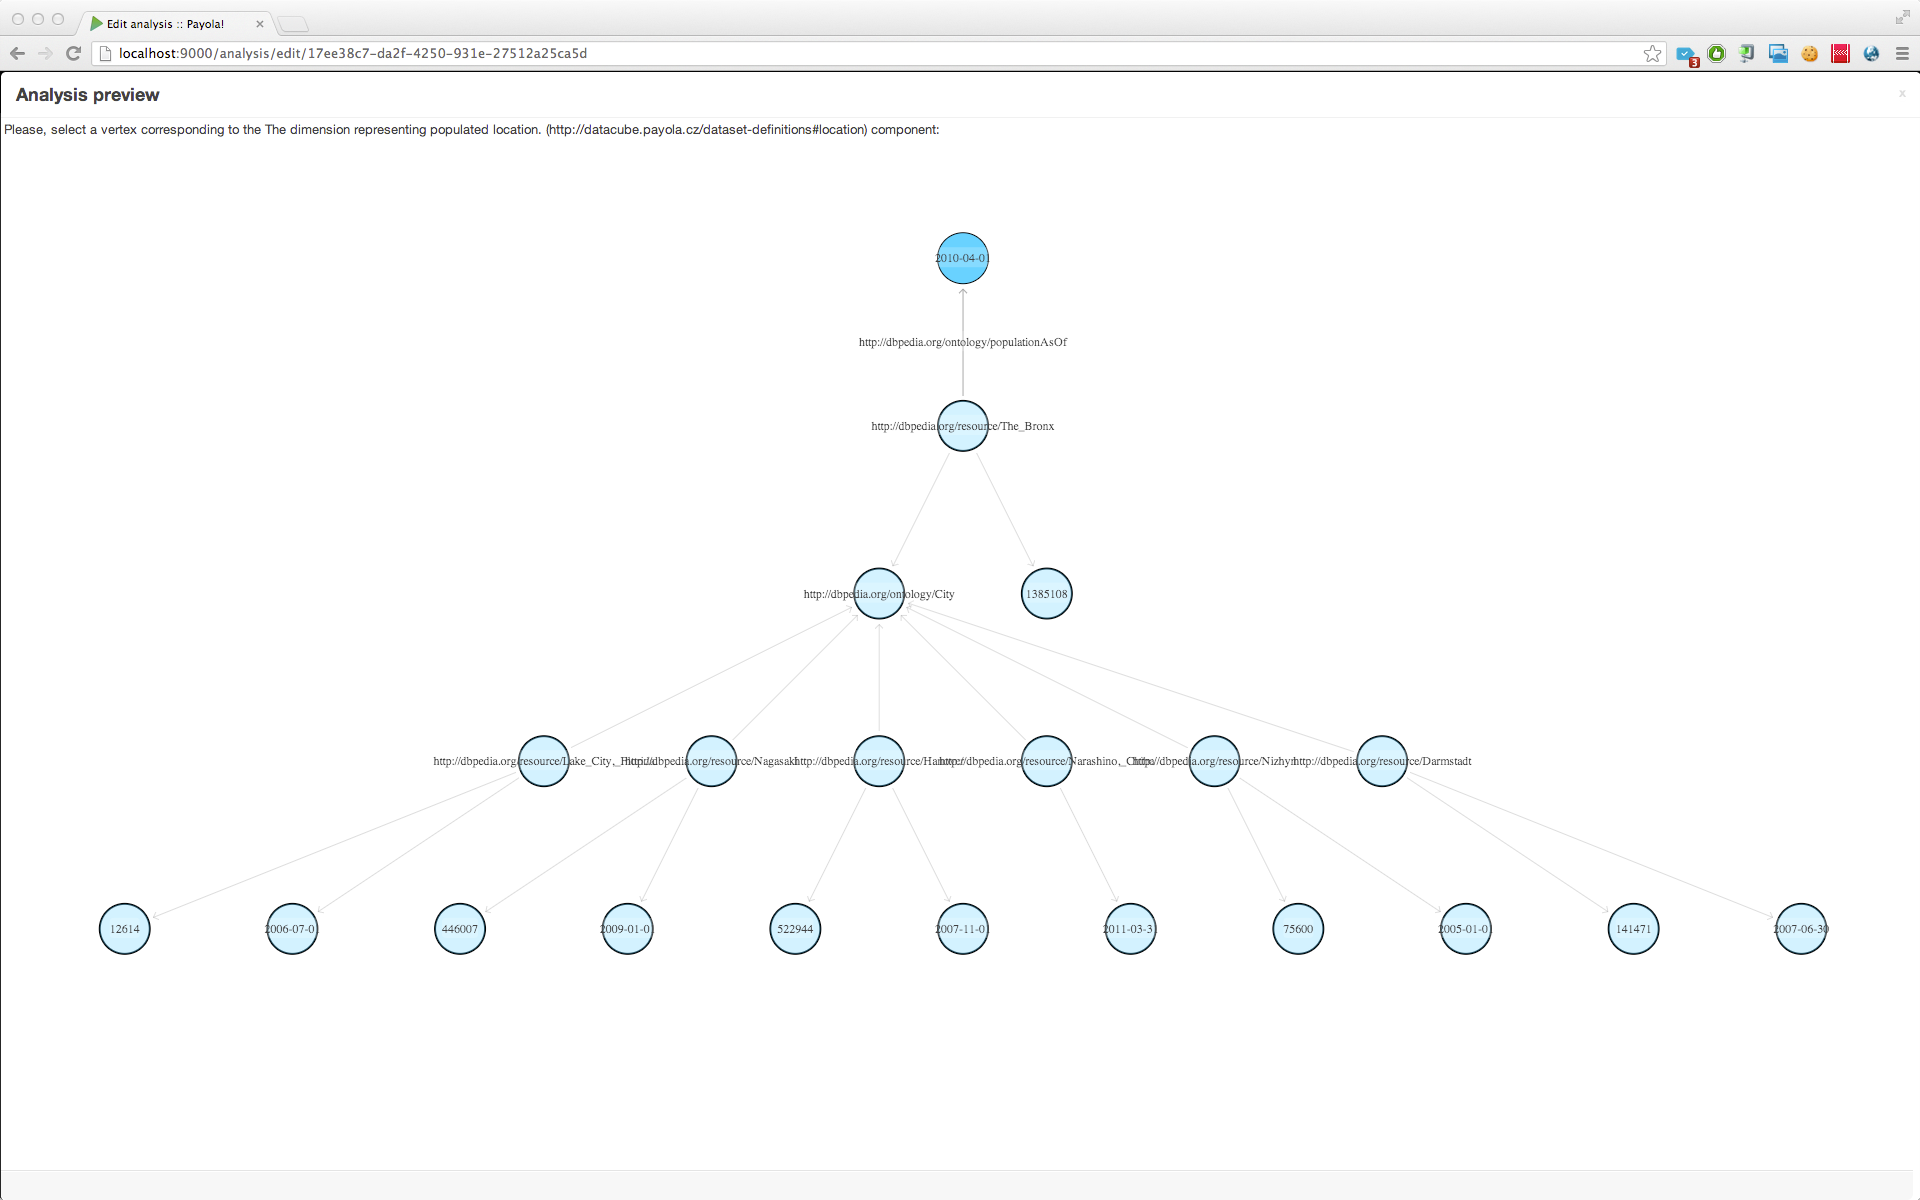
\includegraphics[width=140mm]{img/payola-exp-01-preview.png}
  \caption{An analytical pipeline preview used for a~pattern selection.}
  \label{fig:payola-exp-01-preview}
\end{figure}

\begin{figure}
  \centering
  \includegraphics[width=50mm]{img/payola-exp-01-selection.png}
  \caption{An example provided by~the user in~a form of~a pattern.}
  \label{fig:payola-exp-01-selection}
\end{figure}

\scriptsize
\begin{verbatim}
  CONSTRUCT {
     []  a~ <http://purl.org/linked-data/cube#Observation> ;
         <http://purl.org/linked-data/cube#dataSet> <http://live.payola.cz/analysis/...> ;
         <http://datacube.payola.cz/dataset-definitions#location> ?v1 ;
         <http://datacube.payola.cz/dataset-definitions#period> ?v3 ;
         <http://datacube.payola.cz/dataset-definitions#populationSize> ?v4 .
     } where {
         {
             SELECT DISTINCT ?v1 ?v3 ?v4 {
                ?v1 <http://www.w3.org/1999/02/22-rdf-syntax-ns#type> ?v2 .
                ?v1 <http://dbpedia.org/ontology/populationAsOf> ?v3 .
                ?v1 <http://dbpedia.org/ontology/populationTotal> ?v4 .
            }
       }
  } 
\end{verbatim}
\normalsize

The transformation is~made in~another step of~the analytical pipeline. The~whole evaluation is~done in~seconds. An~exact measurement would not be~conclusive since it~depends on~the actual load of~the DBPedia. The~endpoint 
returns in~about 150 entities no~matter what we~do because that is~the final
count of~entities with the~required properties.

As a~result, we~get a~dataset compliant with the~Data Cube Vocabulary standard. 
We made a~visualization of~the dataset in~both new visualizers. The~results are 
shown in~Figure~\ref{fig:payola-exp-01-vis} and Figure~\ref{fig:payola-exp-01-vis2}.

\begin{figure}
  \centering
  \includegraphics[width=140mm]{img/payola-exp-01-vis.png}
  \caption{Experiment 1: visualization with the~TimeHeatmap plugin.}
  \label{fig:payola-exp-01-vis}
\end{figure}

\begin{figure}
  \centering
  \includegraphics[width=140mm]{img/payola-exp-01-vis2.png}
  \caption{Experiment 1: visualization with the~Universal DataCube plugin.}
  \label{fig:payola-exp-01-vis2}
\end{figure}

In this experiment, we~proved that the~system is~capable of~converting an~arbitrary RDF dataset to~a format compliant with the~Data Cube Vocalbulary 
standard. We~took advantage of~the integration with the~Payola application in~order to~obtain a~meaningful preview.

The system performed well on~the dataset provided by~the DBPedia endpoint, but 
it is~important to~remember that the~endpoint returned a~small amount of~resources. The~quality of~the DBPedia datasets differs a~lot and many 
statistical data are present in~a non--user--friendly form, e.g. while using the~property~\texttt{2000pop}. It~might be~interesting to~use Payola to~discover 
all those properties and build an~analytical pipeline, which will unify all the~approaches. When unified, the~implemented system can be~used in~order to~transform the~data into~the~form of~DCV and/or visualize those.

We have also shown that our visualizers work with real--life data. Based on~what we~have experienced, we~will propose some future user experience 
improvements in~Chapter~\ref{ch:future}. One of~those is~optimizing a~longer running 
geocoding process, which transforms the~city names into~GPS cooridinates.

\section{COINS -- UK~government spending}
Many organizations including governments produce a~lot of~statistical datasets 
focused on~spendings. Therefore, we~wanted to~examine the~behaviour of~the 
system when applied on~such a~dataset. We~chose to~use a~dataset named 
COINS~\cite{coins}. It~is the~database for UK~Government expenditure.

The \url{data.gov.uk} project also made the~dataset available in~a form of~Linked 
Data. Moreover, it~is published in~a form compliant with Data Cube Vocabulary.
Therefore, it~is not necessary to~do a~transformation of~the dataset. But we~tried to~use the~implemented system to~extract the~data from the~original 
dataset.

It is~possible to~use only the~universal visualizer to~visualize the~data 
contained in~the dataset, but we~would need to~extract them manually. In~fact, 
we tried to~do that and we~had to~construct a~SPARQL query, which is~shown in
Figure~\ref{fig:custom-coins-query}. It~allows us~to extract the~data for a~specific data structure 
definition and visualize them. The~result of~such a~visualization is~shown in~Figure~\ref{fig:payola-exp-02}. 

\begin{figure}
  \centering
  \includegraphics[width=140mm]{img/payola-exp-02.png}
  \caption{Experiment 2: visualization of~a custom query with the~Universal DataCube plugin.}
  \label{fig:payola-exp-02}
\end{figure}

\begin{figure}
  \centering
  \includegraphics[width=140mm]{img/payola-exp-02-pattern.png}
  \caption{Experiment 2: Selecting an~exemplary pattern in~a complex graph might be~difficult, yet possible.}
  \label{fig:payola-exp-02-pattern}
\end{figure}

\begin{figure}
  \centering
  \includegraphics[width=140mm]{img/payola-exp-02-result.png}
  \caption{Experiment 2: Visualization of~the extracted dataset.}
  \label{fig:payola-exp-02-result}
\end{figure}

\begin{figure}
  \scriptsize
\begin{verbatim}
PREFIX  coins-dimension: <http://finance.data.gov.uk/dsd/coins/dimension/>
PREFIX  coins-measure: <http://finance.data.gov.uk/dsd/coins/measure/>
PREFIX  source: <http://source.data.gov.uk/>
PREFIX  coins-attribute: <http://finance.data.gov.uk/dsd/coins/attribute/>
PREFIX  qb:   <http://purl.org/linked-data/cube#>

CONSTRUCT 
  { ?obs qb:dataSet ?ds .
    ?obs a~qb:Observation .
    ?obs coins-dimension:dataType <http://finance.data.gov.uk/def/coins/data-type/outturn> .
    ?obs coins-measure:amount ?amount .
    ?obs coins-dimension:departmentLabel ?deptLongName .
    ?obs coins-attribute:budgetBoundaryLabel ?boundaryLabel .
    ?obs coins-attribute:resourceCapitalLabel ?rcLabel . }

WHERE
  { ?obs qb:dataSet ?ds .
    ?obs coins-dimension:departmentCode ?dept .
    ?obs coins-dimension:dataType <http://finance.data.gov.uk/def/coins/data-type/outturn> .
    ?obs coins-measure:amount ?amount .
    ?obs coins-attribute:budgetBoundary ?boundary .
    ?obs coins-attribute:resourceCapital ?rc
    GRAPH <http://source.data.gov.uk/finance/coins/2010-06-14/schema>
      { ?boundary <http://www.w3.org/2000/01/rdf-schema#label> ?boundaryLabel .
        ?rc <http://www.w3.org/2000/01/rdf-schema#label> ?rcLabel .
        ?dept <http://www.w3.org/2000/01/rdf-schema#comment> ?deptLongName
      }
  }
\end{verbatim}
\caption{A custom SPARQL query used to~extract DCV from the~COINS dataset.}
\label{fig:custom-coins-query}
\end{figure}

As stated before, we~tried to~use the~implemented system in~order to~obtain 
similar results. Since the~original dataset is~very large, we~had to~prepare an~analysis in~order to~get a~reasonable preview for a~pattern selection. The~analysis contained only one step. We~added a~SPARQL query plugin. The~query is~presented
in Figure~\ref{fig:coins-query-narrow}.

\begin{figure}
  \scriptsize
\begin{verbatim}
  CONSTRUCT { ?o ?p ?x }
  WHERE
  { ?o qb:dataSet <http://source.data.gov.uk/dataset/coins/fact-table-extract-2009-10> ;
        ?p ?x .
  }
\end{verbatim}
\caption{A custom SPARQL query used for narrowing the~original dataset.}
\label{fig:coins-query-narrow}
\end{figure}

By executing such a~query, we~obtained all triples from the~endpoint 
related to~the specified dataset. We~made a~strong constraint for bringing 
down the~volume of~returned entries. By~using the~\texttt{qb:dataSet} property, 
we automatically filtered the~observations.

Despite the~narrowed dataset, the~preview was still too large 
for the~resulting visualization to~be well--arranged. A~screenshot of~the 
preview can be~seen in~Figure~\ref{fig:payola-exp-02-pattern}. After a~while,
we managed to~select the~desired 
pattern. The~SPARQL query shown in~Figure~\ref{fig:coins-pattern-result} was 
constructed.

\begin{figure}
  \scriptsize
\begin{verbatim}
  CONSTRUCT {
    [] a~<http://purl.org/linked-data/cube#Observation> ;
    <http://purl.org/linked-data/cube#dataSet> <http://live.payola.cz/analysis/...> ;
    <http://finance.data.gov.uk/dsd/coins/dimension/departmentCode> ?v2 ;
    <http://finance.data.gov.uk/dsd/coins/dimension/dataType> ?v3 ;
    <http://finance.data.gov.uk/dsd/coins/measure/amount> ?v4 .
} WHERE {
    {
        SELECT DISTINCT ?v2 ?v3 ?v4 {
            ?v1 <http://finance.data.gov.uk/dsd/coins/dimension/departmentCode> ?v2 .
            ?v1 <http://finance.data.gov.uk/dsd/coins/dimension/dataType> ?v3 .
            ?v1 <http://finance.data.gov.uk/dsd/coins/measure/amount> ?v4 .
        }
    }
} 
\end{verbatim}
\caption{A SPARQL query constructed based on~the pattern selection dialog.}
\label{fig:coins-pattern-result}
\end{figure}

As one can see, the~query differs from the~one we~were about to~simulate. We~did not select available labels. On~the other hand, we~obtained a~more general 
query, which does not fix a~value of~the \texttt{dataType} dimension. That means 
that the~user is~able to~slice the~results of~such an~analysis with the~universal 
visualizer in~order to~obtain the~same visualization as~was in~the case of~the custom 
query. Moreover, they are able to~explore a~much wider range of~data.  

\begin{sloppypar}
Unfortunately, as~the original dataset is~way too large it~was not possible to~fetch all the~related data. The~SPARQL endpoint \mbox{\url{http://openuplabs.tso.co.uk/}}
is placed behind an~Apache proxy, which monitors the~load of~the underlying 
triplestore caused by~executing a~query. After a~while we~hit the~limit and had a~restricted access to~the endpoint for a~few minutes. Therefore, we~had to~limit 
the size of~the extracted dataset. We~managed to~get $10000$ in~the Payola's 
default limit (30 seconds). Most of~the time was spent on~obtaining all the~data from the~endpoint, the~extraction to~DCV was completed in~a matter of~seconds. Also, the~universal visualizer performed well on~a dataset that large.
We made a~screenshot of~a visualization that was prepared during this experiment.
It can be~seen in~Figure~\ref{fig:payola-exp-02-result}.
\end{sloppypar}

We learnt that the~system is~capable of~mapping larger datasets in~a reasonable 
time. But we~also found out that the~preview mechanism will need further 
modifications in~order to~handle larger previews in~a more user--friendly way. 
Performance of~the universal visualizer was acceptable for the~user interface 
responded continuously without any lags. However, we~hit the~limit of~the 
endpoint and were not able to~obtain the~complete dataset. 

The proper way of~working with this dataset would require a~fully faceted 
browser connected directly to~the original SPARQL endpoint. Since it~contains 
DCV data, the~system would be~able to~automatically discover used vocabularies 
and offer them to~the user. On~the other hand, the~vocabularies are not published
separately, which made our task a~bit harder. Implementing an~advanced browser
with an~exploration mode will definitely become the~next step in~the future work. It~would be~very useful to~give the~user a~tool, which will help them 
discover vocabularies and related data in~datasets, which are already compliant 
with Data Cube Vocabulary.

The recommended way of~solving the~large dataset problem with the~current state of~the system
is to~place the~DCV 
plugin into~a~more suitable point. The~preceding operations should narrow the~dataset more naturally by~setting semantical constraints.

In this experiment, we~tried to~use the~implemented system in~a slightly 
different use case. We~used it~in order to~extract a~dataset which is~already in~a form of~Data Cube Vocabulary. Despite the~fact that the~tool was not 
originally meant for this, we~managed to~fulfill our goal. On~the other hand, 
we discovered some user experience flaws, which will be~eliminated in~the future 
development of~the whole Payola framework.

\section{Czech public contracts}
As we~are able to~access the~data related to~public contracts realized in~the 
Czech Republic, we~want to~demonstrate on~them the~possibilities of~the implemented system.
The dataset was created by~scraping website produced by~an online system focused 
on publishing details about public contracts. Therefore, the~form of~the data is~natural and does not come out from a~statistical form.

At first, we~wanted to~extract the~data by~using a~very simple analysis
containing a~sole plugin, an~\emph{ontological filter}. Unfortunately, the~length
of the~generated SPARQL query exceeds the~limit of~the queried SPARQL endpoint.
We extracted the~generated query and tried to~shorten it~by applying prefixes 
and removing whitespace characters. However, after overcoming this challenge, we~hit another limit --- the~underlying Virtuoso endpoint refused to~run the~query 
due to~a large estimated time of~transaction execution.

That is~why we~had to~construct a~custom query in~order to~obtain the~required 
data for making a~preview and a~transformation. We~designed the~query to~gather as~much data as~possible while keeping the~important statistical facts in~all of~the returned entries. The~query is~shown in~Figure~\ref{fig:contracts-query}. It~returns the~details of~about $40000$ public 
contracts.

\begin{figure}
  \scriptsize
  \begin{verbatim}
PREFIX contract: <http://purl.org/procurement/public-contracts#>
PREFIX rdfs: <http://www.w3.org/2000/01/rdf-schema#>
PREFIX dcterms: <http://purl.org/dc/terms/>
prefix vcard: <http://www.w3.org/2006/vcard/ns#> 
prefix gr:	<http://purl.org/goodrelations/v1#> 
prefix ns4:	<http://purl.org/procurement/public-contracts-eu#>

CONSTRUCT 
{
   ?v1 a~contract:Contract .
   ?v1 contract:location ?vloc .
   ?vloc rdfs:label ?locLabel .
   ?vloc ns4:hasParentRegion ?reg .
   ?v1 contract:startDate ?v17 .
   ?v1 contract:estimatedPrice ?ep .
   ?ep gr:hasCurrencyValue	?epv.
}
WHERE
{
   ?v1 a~contract:Contract .
   ?v1 contract:location ?vloc .
   ?vloc rdfs:label ?locLabel .
   ?vloc ns4:hasParentRegion ?reg .
   ?v1 contract:startDate ?v17 .
   ?v1 contract:estimatedPrice ?ep .
   ?ep gr:hasCurrencyValue	?epv.
}
  \end{verbatim}
  \caption{A query constructed to~obtain a~dataset containing desired data.}
  \label{fig:contracts-query}
\end{figure}

We also had to~construct a~custom Data Cube vocabulary with a~data structure 
definition. We~present the~vocabulary in~Figure~\ref{fig:contracts-dcv}.

\begin{figure}
  \scriptsize
  \begin{verbatim}
@prefix rdf:     <http://www.w3.org/1999/02/22-rdf-syntax-ns#> .
@prefix rdfs:    <http://www.w3.org/2000/01/rdf-schema#> .
@prefix xsd:     <http://www.w3.org/2001/XMLSchema#> .
@prefix payola-dcv:   <http://datacube.payola.cz/dataset-definitions#> .
@prefix qb:              <http://purl.org/linked-data/cube#> .
@prefix sdmx:            <http://purl.org/linked-data/sdmx#> .
@prefix sdmx-concept:    <http://purl.org/linked-data/sdmx/2009/concept#> .
@prefix sdmx-dimension:  <http://purl.org/linked-data/sdmx/2009/dimension#> .
@prefix sdmx-measure:    <http://purl.org/linked-data/sdmx/2009/measure#> .
@prefix pc: <http://purl.org/procurement/public-contracts#> .
@prefix ns4: <http://purl.org/procurement/public-contracts-eu#> .
@prefix nuts:     <http://ec.europa.eu/eurostat/ramon/ontologies/geographic.rdf#> .

payola-dcv:ContractsDatastructureDefinition a~qb:DataStructureDefinition ;
  rdfs:label "The definition of~the DS~of a~dataset containing information about public contracts."@en ;
  # Dimensions
  qb:component [
    qb:dimension payola-dcv:location;
    qb:order 1 ;
    rdfs:label "The dimension representing location, where the~money was spent."
  ] ;
  qb:component [  
    qb:dimension payola-dcv:period;
    qb:order 2 ;
    rdfs:label "The dimension representing the~time of~realizing the~contract."
  ] ;
  # Measure
  qb:component [
    qb:measure payola-dcv:price;
    rdfs:label "The measure representing the~price spent on~realizing the~contract."@en
  ] ;
  qb:component [
    qb:attribute payola-dcv:contract;
    rdfs:label "The attribute linking the~observation with a~corresponing contract."@en
  ] ;
  qb:component [
    qb:attribute payola-dcv:region;
    rdfs:label "The attribute specifying the~region, where the~contract was realized."@en
  ] ;
  qb:component [
    qb:attribute payola-dcv:currency;
    rdfs:label "Currency of~the price."@en
  ] .

payola-dcv:location a~rdf:Property, qb:DimensionProperty ;
  rdfs:label "reference location"@en ;
  qb:concept sdmx-concept:refArea .

payola-dcv:period a~rdf:Property, qb:DimensionProperty ;
  rdfs:label "reference period"@en ;
  qb:concept sdmx-concept:refPeriod .

payola-dcv:price a~rdf:Property, qb:MeasureProperty ;
  rdfs:label "price"@en ;
  rdfs:subPropertyOf sdmx-measure:obsValue ;
  rdfs:range xsd:nonNegativeInteger ;
  qb:concept sdmx-concept:valuation .

payola-dcv:contract a~rdf:Property, qb:AttributeProperty ;
  rdfs:label "corresponding public contract"@en ;
  rdfs:range pc:Contract ;
  qb:concept sdmx-concept:comment .
  
payola-dcv:region a~rdf:Property, qb:AttributeProperty ;
  rdfs:label "Parent NUTS region."@en ;
  rdfs:range nuts:NUTSRegion;
  qb:concept sdmx-concept:refArea .
  \end{verbatim}
  \caption{Public contracts data structure definition.}
  \label{fig:contracts-dcv}
\end{figure}

After we~had prepared all the~prerequisities, we~proceeded with transforming the~original dataset to~the form compliant with Data Cube Vocabulary. Based on~the 
data structure definition, we~created a~corresponding plugin, which was then 
inserted into~an~analysis. The~preview contained one of~the selected entries, 
therefore it~was an~easy task to~select a~mapping pattern. One step of~the 
pattern selection process is~pictured in~Figure~\ref{fig:contracts-pattern}.
As a~result, the~system gave us~the SPARQL query show in~Figure~\ref{fig:contracts-query-pattern}.

\begin{figure}
  \centering
  \includegraphics[width=140mm]{img/contracts-pattern.png}
  \caption{Experiment 3: Pattern selection.}
  \label{fig:contracts-pattern}
\end{figure}

\begin{figure}
  \scriptsize
  \begin{verbatim}
CONSTRUCT {
    [] a~<http://purl.org/linked-data/cube#Observation> ;
       qb:dataSet <http://live.payola.cz/analysis/...> ;
       <http://datacube.payola.cz/dataset-definitions#location> ?v2 ;
       <http://datacube.payola.cz/dataset-definitions#period> ?v4 ;
       <http://datacube.payola.cz/dataset-definitions#price> ?v6 ;
       <http://datacube.payola.cz/dataset-definitions#contract> ?v3 ;
       <http://datacube.payola.cz/dataset-definitions#region> ?v7 ;
} where {
   {
      SELECT DISTINCT ?v2 ?v4 ?v6 ?v3 ?v7 {
         ?v1 <http://www.w3.org/2000/01/rdf-schema#label> ?v2 .
         ?v3 <http://purl.org/procurement/public-contracts#location> ?v1 .
         ?v3 <http://purl.org/procurement/public-contracts#startDate> ?v4 .
         ?v3 <http://purl.org/procurement/public-contracts#estimatedPrice> ?v5 .
         ?v5 <http://purl.org/goodrelations/v1#hasCurrencyValue> ?v6 .
         ?v2 <http://purl.org/procurement/public-contracts-eu#hasParentRegion> ?v7 .
      }
   }
} 
  \end{verbatim}
  \caption{Experiment 3: Transformation query.}
  \label{fig:contracts-query-pattern}
\end{figure}

The conversion of~all the~resources in~the source lasted around 300 seconds. We~have noticed that it~took about 200 seconds to~make the~mapping itself, the~rest 
was spent on~fetching the~data.

We tried to~visualize the~dataset in~both implemented Data Cube visualizers. At~first, we~experimented 
with the~TimeHeatmap visualizer. While working with the~large dataset, we~experienced some user discomfort. The~UI was unresponsive for a~short period of~time
(that is~caused by~the single--threaded JavaScript processing concept and would require
involving Web Workers to~avoid). 
In order to~geocode the~locations from the~result, we~had to~increase the~maximum size of~a POST request allowed in~the application. We~present samples of~created visualizations in~Figure~\ref{fig:contracts-map-world} and 
Figure~\ref{fig:contracts-map-zoomed}.

The geocoding process was done in~an acceptable time, but the~size of~the 
dataset caused that the~Google Maps visualization had troubles with zooming. It~had to~recompute all the~40000 of~locations with every zoom.

\begin{figure}
  \centering
  \includegraphics[width=140mm]{img/contracts-map-world.png}
  \caption{Experiment 3: Map expressing the~amount of~money spent by~the Czech Republic in~the world.}
  \label{fig:contracts-map-world}
\end{figure}

\begin{figure}
  \centering
  \includegraphics[width=100mm]{img/contracts-map-zoomed.png}
  \caption{Experiment 3: Map from Figure~\ref{fig:contracts-map-world} zoomed to~the level of~the Czech Republic.}
  \label{fig:contracts-map-zoomed}
\end{figure}

The size of~the dataset caused a~performance drop also in~the case of~the
Universal Data Cube visualizer. Despite the~fact, we~are able to~slice it~and 
take advantage of~the Data Cube Vocabulary format. An~example of~a visualization 
made by~the Universal Data Cube visualizer is~shown in~Figure~\ref{fig:contracts-uni-dcv}.

\begin{figure}
  \centering
  \includegraphics[width=140mm]{img/contracts-uni-dcv.png}
  \caption{Experiment 3: Universal Data Cube visualizer.}
  \label{fig:contracts-uni-dcv}
\end{figure}

In this experiment, we~confirmed that the~implemented system is~capable of~transforming an~arbitrary RDF dataset into~a~form compliant with a~selected Data 
Cube vocabulary. We~also examined the~system while working with a~larger 
dataset. We~confirmed some aforementioned assumptions about the~performance of~the system. Therefore, we~confirmed that we~have correctly identified all the~bottlenecks predicted while preparing the~proposal of~integrating the~system with Payola. 
We will account them in~the future improvements.


\chapter{Future work}
\label{ch:future}

Based on the restrictions of the Payola framwork mentioned in Chapter~\ref{ch:implementation}
and based on experiments with the implemented system (some of them are described in
Chapter~\ref{ch:experiments}), we learned what needs to be done in the future in order to improve
the qualities of the implemented system.

The most crucial lacking feature is a fully faceted browser. We had to adopt the 
design flaw of Payola, which is not capable of caching the results of an analysis. 
Therefore, the user is forced to work with all the results at once, which may 
cause poor performance of the system. We need the Payola framework to adopt some 
existing approaches in order to deliver such a feature. One of them was 
mentioned before --- the integration of a caching mechanism (SESAME, Virtuoso, etc.).

That will dramatically increase the capabilities of the implemented system, 
because it will be possible to work with a proper portion of the data. The user will 
be potentially able to preview the whole dataset while selecting a pattern. A 
really important fact is that the visualizers will be able to query the data 
based on the current state of the visualization, which will significantly help 
to increase the performance of the whole system. One of the features that could 
be done immediately is an improvement to the listings of the detected values of the 
Universal DCV visualizer --- also more sophisticated component than a list of 
checkboxes should be used.

In order to improve the experience of the preview, we can use some advanced 
techniques described in~\cite{faceted-ldow2009}, for instance an ordering by 
\texttt{IRI:RANK}.

Another task will be to undergo a user evaluation in order to reveal other 
missing features and imperfections. Not only based on that, we should continue 
improving the existing visualizers and introduce others for
domain--specific visualisations. The list of requested visualizers will form 
on--the--fly, while exploring other datasets. Such a process will also suggest 
other modifications to the existing visualizers. One comes to mind instantly --- we 
should be able to take advantage of more metadata, for instance measure and 
dimension datatypes, ranges, etc. It is also possible to integrate other types 
of charts.

It would be also possible to propose some procedures, which will examine a given 
dataset and try to convert it to Data Cube Vocabulary automatically. It will 
almost certainly require a more sophisticated integration with the LodVis 
project.

We will also continue to improve Payola features, which are not related with 
Data Cube Vocabulary. Based on the feedback from the ESWC 2013 conference, where the 
Inner analysis feature was presented, people found these modifications and 
features interesting and would like to use them.

Some of those improvements will require Payola to undergo a heavy refactoring, 
when the most adjusted subsystems would be the data access layer and the analytical 
pipeline evaluator.



% Ukázka použití některých konstrukcí LateXu (odkomentujte, chcete-li)
% %%% Ukázka použití některých konstrukcí LaTeXu

\subsection{Ukázka \LaTeX{}u}
\label{ssec:ukazka}

This short subsection serves as an~example of basic \LaTeX{} constructs,
which can be useful for writing a~thesis.

Let us start with lists:

\begin{itemize}
\item The logo of Matfyz is displayed in figure~\ref{fig:mff}.
\item This is subsection~\ref{ssec:ukazka}.
\item Citing literature~\cite{lamport94}.
\end{itemize}

Different kinds of dashes:
red-black (short),
pages 16--22 (middle),
$45-44$ (minus),
and this is --- as you could have expected --- a~sentence-level dash,
which is the longest.
(Note that we have follwed \texttt{a} by a~tilde instead of a~space
to avoid line breaks at that place.)

\newtheorem{theorem}{Theorem}
\newtheorem*{define}{Definition}	% Definice nečíslujeme, proto "*"

\begin{define}
A~{\sl Tree} is a connected graph with no cycles.
\end{define}

\begin{theorem}
This theorem is false.
\end{theorem}

\begin{proof}
False theorems do not have proofs.
\end{proof}

\begin{figure}
	\centering
	\includegraphics[width=30mm]{../img/logo.eps}
	\caption{Logo of MFF UK}
	\label{fig:mff}
\end{figure}


\chapter*{Conclusion}
\addcontentsline{toc}{chapter}{Conclusion}

We have implemented the~proposed system. We~have thusly introduced a~tool which is, with
a user input, able to~convert an~arbitrary RDF dataset into~a~form compliant with Data Cube Vocabulary.
As a~part of~our long--term research, we~decided to~integrate it~into~a~larger system (Payola)
in order to~benefit from such an~integration.
For example, the~user is~able to~make the~conversion as~a~part of~a~larger 
analytical process. It~enables the~user to~work with the~statistical data in~a~usual way. Moreover, they are able to~work with data from multiple datasets at~once.

We have also examined several already existing tools but did not find any~that would 
enable the~user to~perform such a~conversion. There were some related tools 
focused on~a~very similar task and~we~used the~knowledge gained from
examining them. Especially, we~used the~query--by--example principle in~order to~deliver our system
to~our advantage.

During the~process of~implementation, we~have managed to~extend Payola, our RDF application. 
We not only added the~Data Cube Vocabulary related features but also included some 
other useful user experience improvements. Moreso, we~integrated a~completely 
new approach (in the~scope of~Payola) a~construction of~a~SPARQL query, which can 
be reused in~other scenarios in~order to~deliver some new features.

Based on~our experience and~our research, we~have also determined those parts of~Payola,
which are in~need of~an~improvement or~redesign for providing a~more 
efficient behaviour. That is~also crucial in~order to~improve the~reliability, 
the~performance and~the~usability of~the~implemented system while working on~this 
thesis.

Last, but not least, we~delivered two new visualizer plugins, which enable the~user to~explore the~Data Cube Vocabulary related datasets. Whilst the~first one tends to~be~universal, the~second one is~focused on~visualizing geospatial data. Improving 
the user experience of~those visualizers should become the~core of~the~future work, 
including an~implementation of~a~fully faceted browser. To~offer a~visualizer,
which may probably be~considered a~basis for a~sophisticated faceted browser for cube data,
represents a~significant achievement.

We fulfilled the~goal of~this thesis. In~spite of~the~fact that the~system will be~eventually improved
as it~happens with every other new system, we~find
the implementation satisfactory to~the~current state of~the~Payola framework. We~consider the~provided feature to~be~of~a~great benefit to~the~Payola users.


%%% Seznam použité literatury
%%% Seznam použité literatury je zpracován podle platných standardů. Povinnou citační
%%% normou pro diplomovou práci je ISO 690. Jména časopisů lze uvádět zkráceně, ale jen
%%% v kodifikované podobě. Všechny použité zdroje a prameny musí být řádně citovány.

\def\bibname{Bibliography}
\begin{thebibliography}{99}
\addcontentsline{toc}{chapter}{\bibname}

\bibitem{rdf}
{\sc W3C}. 
Resource Description Framework (RDF): \emph{Semantic Web Standards}.
W3C - RDF CORE WORKING GROUP. 
\emph{W3C - Semantic Web Standards} [online].
2013, 22.3.2013 [cit. 2013-05-22].
Available from: \url{http://www.w3.org/RDF/}

\bibitem{ld}
{\sc HEATH,} Tom.
LINKED DATA COMMUNITY. \emph{Linked Data: Connect Distributed Data across the Web}
[online]. 2013 [cit. 2013-02-3]. 
Available from: \url{http://linkeddata.org/}

\bibitem{dcv}
{\sc W3C.}
The RDF Data Cube Vocabulary:
\emph{W3C Candidate Recommendation 25 June 2013} [online]. 2013
[cit. 2013-07-26]. Available from: \url{http://www.w3.org/TR/vocab-data-cube/}

\bibitem{payola}
{\sc ŠIROKÝ}, Jan, Jiří HELMICH, Ondřej HEŘMÁNEK, Ondřej KUDLÁČEK and Kryštof VÁŠA.
PAYOLA. \emph{Payola} [online]. Prague, 2012 [cit. 2013-07-26]. 
Available from: \url{http://www.payola.cz/}

\bibitem{ldvm}
 {\sc FERNÁNDEZ,} Josep Maria Brunetti, Sören AUER and Roberto GARCIA.
 \emph{The Linked Data Visualization Model}
 [online]. Lleida, Spain; Leipzig, Germany, 2012
 [cit. 2013-04-13].
 Available from: \url{http://iswc2012.semanticweb.org/sites/default/files/paper_29.pdf}

\bibitem{un}
{\sc UNITED NATIONS.}
\emph{United Nations: We the peoples... A stronger UN for a better world.} [online].
New York, 2013 [cit. 2013-05-22]. 
Available from: \url{http://www.un.org/en/}

\bibitem{pubdata} 
  {\sc } GOOGLE INC.
  \emph{Google Public Data Explorer}
  [online]. 2013 [cit. 2013-04-13]. Available from: \url{http://www.google.com/publicdata/explore}

\bibitem{lod2}
{\sc UNIVERSITY OF LEIPZIG}
\emph{LOD2: Creating Knowledge out of Interlinked Data} [online]. 2013
[cit. 2013-07-26].
Available from: \url{http://lod2.eu/}

\bibitem{dbpedia}
{\sc DBPEDIA.} 
\emph{DBPedia} [online]. 2013, 2013-05-08 [cit. 2013-01-16]. 
Available from: \url{http://dbpedia.org/}

\bibitem{prefixcc}
  {\sc CYGANIAK,} Richard. DIGITAL ENTERPRISE RESEARCH INSTITUTE. 
  \emph{Namespace lookup for RDF developers}
  [online]. 2013 [cit. 2013-04-13]. Available from: \url{http://prefix.cc/}

\bibitem{lod-cloud}
{\sc CYGANIAK,} Richard a Anja JENTZSCH. LATC, DERI.
\emph{The Linking Open Data cloud diagram} [online]. 2011, 2011-09-19 [cit. 2013-07-27].
Available from: \url{http://lod-cloud.net/}

\bibitem{ldvm2}
 {\sc BRUNETTI,} Josep Maria, Sören AUER, Roberto GARCÍA, Jakub KLÍMEK and Martin NECASKY.
 The Linked Data Visualisation Model.
 \emph{AKSW Subversion Repository} [online]. 2013, č. 1 [cit. 2013-04-14].
 Available from: \url{http://svn.aksw.org/papers/2013/WWW_LDVM/public.pdf}

\bibitem{owl}
{\sc W3C.}
\emph{OWL Web Ontology Language: Overview} [online]. 2004,
2004-02-10 [cit. 2012-12-28].
Available from: \url{http://www.w3.org/TR/owl-features/}

\bibitem{wikipedia}
{\sc WIKIMEDIA FOUNDATION, Inc}
\emph{Wikipedia} [online]. 2012 [cit. 2012-11-22].
Available from:  \url{http://en.wikipedia.org/wiki/Main_Page}

\bibitem{msdn-cube}
{\sc MICROSOFT.}
\emph{MSDN Library: an essential source of information for developers} [online].
Just What Are Cubes Anyway?: A Painless Introduction to OLAP Technology.
2012 [cit. 2012-12-26].
Available from: \url{http://msdn.microsoft.com/en-us/library/aa140038%28v=office.10%29.aspx#odc\_da\_whatrcubes\_topic2}

\bibitem{sdmx}
  {\sc } SDMX INITIATIVE.
  \emph{Statistical Data and Metadata Exchange}
  [online]. 2001 [cit. 2013-04-13]. Available from: \url{www.sdmx.org}

\bibitem{iso}
 {\sc } INTERNATIONAL ORGANIZATION FOR STANDARDIZATION.
 \emph{ISO - International Organization for Standardization}
 [online]. 2013 [cit. 2013-04-13]. Available from: \url{http://www.iso.org}
 
\bibitem{isosdmx}
 {\sc} ISO 17369:2013 - Statistical data and metadata exchange (SDMX).
 INTERNATIONAL ORGANIZATION FOR STANDARDIZATION.
 \emph{ISO - International Organization for Standardization} [online]. 2013 [cit. 2013-04-13].
 Available from: \url{http://www.iso.org/iso/catalogue_detail.htm?csnumber=52500}
 
\bibitem{sdmxuserguide}
 {\sc } SDMX 2.1 User Guide.
 \emph{SDMX 2.1 User Guide}.
 Version 0.1. SDMX, 2012.
 Available from: \url{http://sdmx.org/wp-content/uploads/2012/11/SDMX_2-1_User_Guide_draft_0-1.pdf}

\bibitem{mantra}
 {\sc SHNEIDERMAN,} Ben.
 The eyes have it: A task by data type taxonomy for information visualizations.
 \emph{Proceedings 1996 IEEE Symposium on Visual Languages: proceedings,
 August 14-16, 1996, Blue Mountain Lake, New York}
 [online]. Los Alamitos, Calif.: IEEE Comput. Soc. Press, 1996, s. 336-343
 [cit. 2013-04-13]. ISSN 0-8186-7469-5. DOI: 10.1109/VL.1996.545307.
 Available from: \url{http://ieeexplore.ieee.org/lpdocs/epic03/wrapper.htm?arnumber=545307}

\bibitem{olap2dc-paper}
{\sc SALAS,} Percy E, Michael MARTIN and Fernando Maia Da MOTA.
OLAP2DataCube: An Ontowiki Plug-In for Statistical Data Publishing.
\emph{Proceedings of the 2nd Workshop on Developing Tools as Plug-ins.} 
[online]. 2012, Pages: 79-83 [cit. 2013-07-26]. ISBN:9781467318204.
Available from: \url{http://www.inf.puc-rio.br/~casanova/Publications/Papers/2012-Papers/2012-TOPI-olap.pdf}

\bibitem{tabels-web}
{\sc CTIC.}
\emph{Tabels: Make meaning of tabular data} [online]. [cit. 2012-12-20].
Available from: \url{http://idi.fundacionctic.org/tabels/}

\bibitem{aksw}
{\sc ARNDT, Natanael.} AKSW. 
\emph{Agile Knowledge Engineering and Semantic Web (AKSW)} [online].
2013, 03-2013 [cit. 2013-07-26].
Available from: \url{http://aksw.org}

\bibitem{ontowiki}
{\sc TRAMP,} Sebastian. AKSW.
\emph{OntoWiki: a tool providing support for agile, distributed knowledge engineering scenarios.}
[online]. [cit. 2013-01-04]. 
Available from: \url{http://aksw.org/Projects/OntoWiki.html}

\bibitem{highcharts}
{\sc HIGHSOFT SOLUTIONS AS.}
\emph{Highcharts: Interactive JavaScript charts for your webpage} [online]. 2012
[cit. 2013-07-19]. 
Available from: \url{http://www.highcharts.com/}

\bibitem{lodspeakr}
{\sc GRAVES,} Alvaro. 
\emph{Lodspeakr: Framework to create Linked Data-based applications} [online].
2013 [cit. 2013-04-12]. 
Available from: \url{http://alangrafu.github.io/lodspeakr/}

\bibitem{angularjs}
{\sc GOOGLE.}
\emph{AngularJS: Superheroic JavaScript MVW Framework} [online]. 2011
[cit. 2013-07-01]. Available from: \url{http://angularjs.org/}

\bibitem{geoglobe}
{\sc I2G.}
\emph{Geoglobe} [online]. 2012 [cit. 2013-05-14].
Available from: \url{http://data.i2g.pl/insigos/hz-geo/globe/}

\bibitem{d3}
{\sc BOSTOCK}, Michael. 
\emph{D3.js: Data-Driven Documents} [online]. 2012 [cit. 2013-02-02].
Available from: \emph{http://d3js.org/}

\bibitem{prefuse}
\emph{Prefuse: information visualization toolkit} [online]. 2012, 2012-01-13 [cit. 2013-05-28].
Available from: \url{http://prefuse.org/}

\bibitem{tabulator-paper}
{\sc BERNERS-LEE,} Tim, Yuhsin CHEN, Lydia CHILTON, Dan CONNOLLY,
Ruth DHANARAJ, James HOLLENBACH, Adam LERER and David SHEETS.
Tabulator: Exploring and analyzing linked data on the semantic web.
 [online]. 2006 [cit. 2013-07-26]. 
Available from: \url{http://student.bus.olemiss.edu/files/conlon/others/others/semantic%20web%20papers/Berners-Lee.pdf}

\bibitem{exploratory-search}
{\sc Marchionini,} G. \emph{Exploratory search: From finding to 
understanding.} Comm. Of the ACM, 49(4), 2006.

\bibitem{explorator}
{\sc ARAÚJO,} Samur F. C. de and Daniel SCHWABE.
Explorator: a tool for exploring RDF data through direct  manipulation. 
\emph{LDOW 2009 Proceedings} [online]. 2009, s. 2009 [cit. 2013-04-08].
Available from: \url{http://events.linkeddata.org/ldow2009/papers/ldow2009_paper2.pdf}

\bibitem{sesame}
{\sc ADUNA.}
\emph{OpenRDF.org: home of Sesame} [online]. 2012 [cit. 2013-07-15].
Available from: \url{http://www.openrdf.org/}

\bibitem{mit-simile}
{\sc MIT.}
\emph{SIMILE Widgets: Free, Open-Source Data Visualization Web Widgets, and More}
[online]. 2009 [cit. 2013-06-29]. 
Available from: \url{http://simile-widgets.org/}

\bibitem{exhibit}
{\sc SMITH,} MacKenzie and Eric Miller ZEPHEIRA.
Exhibit 3.0:
\emph{An Open Source Software Platform for Publishing Linked Data}.
In: \emph{emanticweb.com: The Voice of Semantic Web Business} [online].
2011 [cit. 2013-04-26].
Available from: \url{http://semanticweb.com/exhibit-3-0-part-1-an-open-source-software-platform 
-for-publishing-linked-data_b22962}

\bibitem{ckan}
 {\sc OPEN KNOWLEDGE FOUNDATION.}
 The open source data portal software
 \emph{Comprehensive Knowledge Archive}
 [online]. 2013
 [cit. 2013-04-14]. Available from: \url{http://ckan.org/pic03/wrapper.htm?arnumber=545307}

\bibitem{thedatahub}
 {\sc OPEN KNOWLEDGE FOUNDATION.}
The Datahub:
 \emph{The easy way to get, use and share data}
 [online]. 2012
 [cit. 2013-04-14]. Available from: \url{http://datahub.io}

\bibitem{void}
{\sc ALEXANDER,} Keith, Richard CYGANIAK, Michael HAUSENBLAS and Jun ZHAO. W3C.
\emph Describing Linked Datasets with the VoID Vocabulary: W3C Interest Group Note 03 March 2011}
[online]. 2010 [cit. 2013-05-16]. 
Available from: \url{http://www.w3.org/TR/void/}

\bibitem{github-payola} 
{\sc ŠIROKÝ,} Jan, Jiří HELMICH, Ondřej HEŘMÁNEK, Ondřej KUDLÁČEK and Kryštof VÁŠA. PAYOLA.
\emph{Payola GitHub repository} [online]. 2012 [cit. 2012-10-26].
Available from: \url{https://github.com/payola/Payola}

\bibitem{github-lodstats}
{\sc AKSW.}
\emph{LODStats GitHub repository} [online]. 2012 [cit. 2013-06-06].
Available from: \emph{https://github.com/AKSW/LODStats}
 
\bibitem{lodstats}
{\sc AUER,} Sören, Jan DEMTER, Michael MARTIN and Jens LEHMANN. 
LODStats
\emph{An Extensible Framework for High-Performance Dataset Analytics.}
[online]. s. 353 [cit. 2013-07-26]. DOI: 10.1007/978-3-642-33876-2\_31.
Available from: \url{http://jens-lehmann.org/files/2012/ekaw_lodstats.pdf}

\bibitem{yahoo-pipes}
{\sc YAHOO.}
\emph{Pipes: Rewire the web} [online]. 2011 [cit. 2012-10-20].
Available from: \url{http://pipes.yahoo.com/pipes/}

\bibitem{deri-pipes}
{\sc PHUOC,} Danh Le, Christian MORBIDONI, Axel POLLERES,
Matthias Samwald Robert FULLER and Giovanni TUMMARELLO. DERI.
\emph{DERI Pipes: Open Source, Extendable, Embeddable Web Data Mashups} [online].
2011 [cit. 2012-10-12]. 
Available from: \url{http://pipes.deri.org}

\bibitem{deri-screen-source}
{\sc PHUOC,} Danh Le, Christian MORBIDONI, Axel POLLERES,
Matthias SAMWALD, Robert FULLER and Giovanni TUMMARELLO.
\emph{DERI Pipes: Open Source, Extendable, Embeddable Web Data Mashups} [online]. 2011
[cit. 2013-11-12].
Available from: \url{http://pipes.deri.org/cityfacts.html}

\bibitem{lodvis}
{\sc BRUNETTI,} Josep Maria. GRIHO.
\emph{LodVis: prototype that implements the Linked Data Visualization Model (LDVM)}
[online]. 2012 [cit. 2012-09-30].
Available from: \url{http://lodvisualization.appspot.com/}

\bibitem{virtuoso}
{\sc OPENLINK.}
\emph{Virtuoso Universal Server} [online]. 2013 [cit. 2013-01-20].
Available from: \url{http://virtuoso.openlinksw.com/}

\bibitem{payola:ug:join-plugin}
{\sc ŠIROKÝ,} Jan, Jiří HELMICH, Ondřej HEŘMÁNEK, Ondřej KUDLÁČEK a Kryštof VÁŠA. PAYOLA.
\emph{User Guide} [online]. 2012 [cit. 2013-07-27]. 
Available from: \url{https://github.com/payola/Payola/blob/develop/docs/user_guide.md#join}

\bibitem{payola:ug}
{\sc ŠIROKÝ,} Jan, Jiří HELMICH, Ondřej HEŘMÁNEK, Ondřej KUDLÁČEK a Kryštof VÁŠA. PAYOLA.
\emph{User Guide} [online]. 2012 [cit. 2013-07-27]. 
Available from: \url{https://github.com/payola/Payola/blob/develop/docs/user_guide.md}

\bibitem{squeryl}
{\sc LÉVESQUE,} Maxime. 
\emph{Squeryl: A Scala ORM for SQL Databases} [online]. 2012 [cit. 2013-02-10].
Available from: \url{http://squeryl.org/}

\bibitem{payola:dg}
{\sc ŠIROKÝ,} Jan, Jiří HELMICH, Ondřej HEŘMÁNEK, Ondřej KUDLÁČEK a Kryštof VÁŠA. PAYOLA.
\emph{Developer Guide} [online]. 2012 [cit. 2013-07-27]. 
Available from: \url{https://github.com/payola/Payola/blob/develop/docs/developer_guide.md}

\bibitem{jena}
{\scAPACHE SOFTWARE FOUNDATION.} 
\emph{Apache Jena: The core RDF API} [online]. 2011 [cit. 2013-02-27]. 
Available from: \url{http://jena.apache.org/documentation/rdf/}

\bibitem{s2js}
{\sc ŠIROKÝ,} Jan. 
\emph{SWAT: Scala Web Application Toolkit} [online]. 2012 [cit. 2013-07-27].
Available from: \url{https://github.com/siroky/Swat}

\bibitem{federated-queries}
{\sc PRUD'HOMMEAUX,} Eric and Carlos BUIL-ARANDA. W3C.
\emph{SPARQL 1.1 Federated Query: W3C Recommendation 21 March 2013} [online].
2013, 2013-03-21 [cit. 2013-07-26].
Available from: \url{http://www.w3.org/TR/sparql11-federated-query/}

\bibitem{leipzich-uni}
{\sc UNIVERSITÄT LEIPZIG.} \emph{Universität Leipzig} [online]. 2013 [cit. 2013-06-27].
Available from: \url{http://www.zv.uni-leipzig.de/}

\bibitem{playfw}
{\sc TYPESAFE.}
\emph{Play Framework: The High Velocity Web Framework For Java and Scala} [online].
2012 [cit. 2012-11-14]. 
Available from: \uri{http://www.playframework.com/} 

\bibitem{flot}
{\sc LAURSEN,} Ole. IOLA. 
\emph{Flot: Attractive JavaScript plotting for jQuery} [online]. 2007 [cit. 2013-05-06].
Available from: \url{http://www.flotcharts.org/}

\bibitem{rfc-2617}
RFC 2617.
\emph{HTTP Authentication: Basic and Digest Access Authentication}.
The Internet Society, June 1999. [online]
Available from: \url{http://tools.ietf.org/html/rfc2617}

\bibitem{apache-http-commons}
{\scAPACHE SOFTWARE FOUNDATION.}
\emph{HttpClient} [online]. 2011 [cit. 2013-04-10]. 
Available from: \url{http://hc.apache.org/httpclient-3.x/}

\bibitem{coins}
{\sc DATA.GOV.UK.}
\emph{COINS as Linked Data} [online]. 2010, 11-11-2010 [cit. 2013-01-16].
Available from: \url{http://data.gov.uk/resources/coins}

\bibitem{faceted-ldow2009}
{\sc ERLING,} Orri.
Faceted Views over Large-Scale Linked Data.  [online]. [cit. 2013-07-26].
Available from: 
\url{http://events.linkeddata.org/ldow2009/papers/ldow2009_paper3.pdf}

\bibitem{datacube-wiki}
\emph{Data cube} [online]. 2012 [cit. 2013-09-27]. 
Available from: \url{http://en.wikipedia.org/wiki/Data_cube}

\bibitem{vidax}
{\sc DUMAS,} Bruno, Tim BROCHÉ, Lode HOSTE a Beat SIGNER. ViDaX.
\emph{Proceedings of the International Working Conference on Advanced Visual Interfaces - AVI '12}
[online]. New York, New York, USA: ACM Press, 2012, s. 757-
[cit. 2013-05-12]. DOI: 10.1145/2254556.2254702.
Available from: \url{http://dl.acm.org/citation.cfm?doid=2254556.2254702}



\end{thebibliography}


%%% Tabulky v diplomové práci, existují-li.
\chapwithtoc{List of Tables}

%%% Použité zkratky v diplomové práci, existují-li, včetně jejich vysvětlení.
\chapwithtoc{List of Abbreviations}

%%% Přílohy k diplomové práci, existují-li (různé dodatky jako výpisy programů,
%%% diagramy apod.). Každá příloha musí být alespoň jednou odkazována z vlastního
%%% textu práce. Přílohy se číslují.
\chapwithtoc{Attachments}

\openright
\end{document}
